%%%%%%%%%%%%%%%%%%%%%%%%%%%%%%%%%%%%%%%%%
% Programming/Coding Assignment
% LaTeX Template
%
% This template has been downloaded from:
% http://www.latextemplates.com
%
% Original author:
% Ted Pavlic (http://www.tedpavlic.com)
%
% Adapted by:
% Jacopo De Stefani (jacopo.de.stefani@gmail.com)
%
% Note:
% The \lipsum[#] commands throughout this template generate dummy text
% to fill the template out. These commands should all be removed when 
% writing assignment content.
%
% This template uses a Perl script as an example snippet of code, most other
% languages are also usable. Configure them in the "CODE INCLUSION 
% CONFIGURATION" section.
%
%%%%%%%%%%%%%%%%%%%%%%%%%%%%%%%%%%%%%%%%%

%----------------------------------------------------------------------------------------
%	PACKAGES AND OTHER DOCUMENT CONFIGURATIONS
%----------------------------------------------------------------------------------------

\documentclass{article}

\usepackage[utf8]{inputenc}
\usepackage{textcomp}
\usepackage{fancyhdr} % Required for custom headers
\usepackage{lastpage} % Required to determine the last page for the footer
\usepackage{extramarks} % Required for headers and footers
\usepackage[usenames,dvipsnames]{color} % Required for custom colors
\usepackage{graphicx} % Required to insert images
\usepackage{listings} % Required for insertion of code
\usepackage{courier} % Required for the courier font
\usepackage{lipsum} % Used for inserting dummy 'Lorem ipsum' text into the template
\usepackage{rotating}
\usepackage{natbib}
\usepackage{graphicx}
\usepackage{tikz}
\usepackage{pgfplots}
\usepackage{multicol}
\usepackage{caption}
\usepackage{amsmath}
\usepackage{amsfonts}
\usepackage{algpseudocode}% http://ctan.org/pkg/algorithmicx
\usepackage{algorithm}% http://ctan.org/pkg/algorithm
\usepackage{pdflscape}
\usepackage{hyperref}
\usepackage{pifont}
\usepackage{subcaption}

\usetikzlibrary{positioning,shadows,arrows,intersections,calc,automata}

% Margins
\topmargin=-0.45in
\evensidemargin=0in
\oddsidemargin=0in
\textwidth=6.5in
\textheight=9.0in
\headsep=0.25in

\linespread{1.1} % Line spacing

% Set up the header and footer
\pagestyle{fancy}
\lhead{} % Top left header
\chead{\hmwkClass\ (\hmwkClassInstructor\ ): \hmwkTitle} % Top center head
\rhead{}%\firstxmark} % Top right header
\lfoot{\hmwkAuthorName} % Bottom left footer
\cfoot{}%\lastxmark} % Bottom center footer
\rfoot{Page\ \thepage\ of\ \protect\pageref{LastPage}} % Bottom right footer
\renewcommand\headrulewidth{0.4pt} % Size of the header rule
\renewcommand\footrulewidth{0.4pt} % Size of the footer rule

\setlength\parindent{0pt} % Removes all indentation from paragraphs

%----------------------------------------------------------------------------------------
%	CODE INCLUSION CONFIGURATION
%----------------------------------------------------------------------------------------

\definecolor{MyDarkGreen}{rgb}{0.0,0.4,0.0} % This is the color used for comments
\lstloadlanguages{Python} % Load Perl syntax for listings, for a list of other languages supported see: ftp://ftp.tex.ac.uk/tex-archive/macros/latex/contrib/listings/listings.pdf
\lstset{language=Python, % Use Perl in this example
        frame=single, % Single frame around code
        basicstyle=\small\ttfamily, % Use small true type font
        keywordstyle=[1]\color{Blue}\bf, % Perl functions bold and blue
        keywordstyle=[2]\color{Purple}, % Perl function arguments purple
        keywordstyle=[3]\color{Blue}\underbar, % Custom functions underlined and blue
        identifierstyle=, % Nothing special about identifiers                                         
        commentstyle=\usefont{T1}{pcr}{m}{sl}\color{MyDarkGreen}\small, % Comments small dark green courier font
        stringstyle=\color{Purple}, % Strings are purple
        showstringspaces=false, % Don't put marks in string spaces
        tabsize=5, % 5 spaces per tab
        %
        % Put standard Perl functions not included in the default language here
        morekeywords={rand},
        %
        % Put Perl function parameters here
        morekeywords=[2]{on, off, interp},
        %
        % Put user defined functions here
        morekeywords=[3]{test},
       	%
        morecomment=[l][\color{Blue}]{...}, % Line continuation (...) like blue comment
        numbers=left, % Line numbers on left
        firstnumber=1, % Line numbers start with line 1
        numberstyle=\tiny\color{Blue}, % Line numbers are blue and small
        stepnumber=5, % Line numbers go in steps of 5
        breaklines=true
}

% Creates a new command to include a perl script, the first parameter is the filename of the script (without .pl), the second parameter is the caption
\newcommand{\pyscript}[2]{
\begin{itemize}
\item[]\lstinputlisting[caption=#2,label=#1]{#1.py}
\end{itemize}
}

%----------------------------------------------------------------------------------------
%	DOCUMENT STRUCTURE COMMANDS
%	Skip this unless you know what you're doing
%----------------------------------------------------------------------------------------

% Header and footer for when a page split occurs within a problem environment
\newcommand{\enterProblemHeader}[1]{
\nobreak\extramarks{#1}{#1 continued on next page\ldots}\nobreak
\nobreak\extramarks{#1 (continued)}{#1 continued on next page\ldots}\nobreak
}

% Header and footer for when a page split occurs between problem environments
\newcommand{\exitProblemHeader}[1]{
\nobreak\extramarks{#1 (continued)}{#1 continued on next page\ldots}\nobreak
\nobreak\extramarks{#1}{}\nobreak
}

\setcounter{secnumdepth}{0} % Removes default section numbers
\newcounter{homeworkProblemCounter} % Creates a counter to keep track of the number of problems

\newcommand{\homeworkProblemName}{}
\newenvironment{homeworkProblem}[1][Problem \arabic{homeworkProblemCounter}]{ % Makes a new environment called homeworkProblem which takes 1 argument (custom name) but the default is "Problem #"
\stepcounter{homeworkProblemCounter} % Increase counter for number of problems
\renewcommand{\homeworkProblemName}{#1} % Assign \homeworkProblemName the name of the problem
\section{\homeworkProblemName} % Make a section in the document with the custom problem count
\enterProblemHeader{\homeworkProblemName} % Header and footer within the environment
}{
\exitProblemHeader{\homeworkProblemName} % Header and footer after the environment
}

\newcommand{\problemAnswer}[1]{ % Defines the problem answer command with the content as the only argument
\noindent\framebox[\columnwidth][c]{\begin{minipage}{0.98\columnwidth}#1\end{minipage}} % Makes the box around the problem answer and puts the content inside
}

\newcommand{\homeworkSectionName}{}
\newenvironment{homeworkSection}[1]{ % New environment for sections within homework problems, takes 1 argument - the name of the section
\renewcommand{\homeworkSectionName}{#1} % Assign \homeworkSectionName to the name of the section from the environment argument
\subsection{\homeworkSectionName} % Make a subsection with the custom name of the subsection
\enterProblemHeader{\homeworkProblemName\ [\homeworkSectionName]} % Header and footer within the environment
}{
\enterProblemHeader{\homeworkProblemName} % Header and footer after the environment
}

%----------------------------------------------------------------------------------------
%	USER DEFINED TIKZ STYLES
%----------------------------------------------------------------------------------------

\tikzset{
    player1/.style={circle, draw=none, fill=green!70!black, circular drop shadow,
        text centered, anchor=north, text=white},
    player2/.style={circle, draw=none, fill=orange, circular drop shadow,
        text centered, anchor=north, text=white},
    chance/.style={circle, draw,text centered, anchor=north},
    subtreeB/.style={rectangle, draw, rounded corners=1mm, color=red, thick,
        text centered, anchor=north, text=red},
    subtreeC/.style={rectangle, draw, rounded corners=1mm, color=orange, thick,
        text centered, anchor=north, text=orange},
    ex2/.style={circle, draw,text centered, anchor=north},
    nashEq1P/.style={circle,draw=none, fill=green!70!black, text centered, anchor=north, text=white,inner sep=2pt},
    nashEq2P/.style={circle,draw=none, fill=orange, text centered, anchor=north, text=white,inner sep=2pt},
    nashEqPoints/.style={fill=white,draw=black,thick},
    level distance=0.5cm, growth parent anchor=south
}

\tikzstyle{tier}=[draw, fill=yellow!20, text width=6.0em, text centered,
  minimum height=1.5em,drop shadow]
\tikzstyle{component} = [tier, text width=8em, minimum width=10em,
  minimum height=3em, rounded corners, drop shadow,inner sep=2pt]
\tikzstyle{texto} = [above, text width=6em, text centered]
\tikzstyle{linepart} = [draw, thick, color=black!50, -latex', dashed]
\tikzstyle{line} = [draw, thick, color=black!50, -latex', ->]
\tikzstyle{ur}=[draw, text centered, minimum height=0.01em]
 
% Define distances for bordering
\newcommand{\blockdist}{1.3}
\newcommand{\edgedist}{1.5}

\newcommand{\component}[2]{node (p#1) [component]
  {{\scriptsize\textit{#2}}}}


% Draw background
\newcommand{\backgroundSquare}[5]{%
  \begin{pgfonlayer}{background}
    % Left-top corner of the background rectangle
    \path (#1.west |- #2.north)+(-0.5,0.5) node (a1) {};
    % Right-bottom corner of the background rectanle
    \path (#3.east |- #4.south)+(+0.5,-0.25) node (a2) {};
    % Draw the background
    \path[fill=blue!20,rounded corners, draw=black!50, dashed]
      (a1) rectangle (a2);
    \path (a1.east |- a1.south)+(0.8,-0.3) node (u1)[texto]
      {\scriptsize\textit{#5 Tier}};
  \end{pgfonlayer}}


\newcommand*\circled[2]{\tikz[baseline=(char.base)]{
            \node[#2,rectangle, rounded corners=0.7mm, text=white] (char) {#1};}}
\newcommand*\cellvcenter[1]{\raisebox{-\height}{#1}}


\newcommand{\cmark}{\ding{51}}%
\newcommand{\xmark}{\ding{55}}%

%----------------------------------------------------------------------------------------
%	NAME AND CLASS SECTION
%----------------------------------------------------------------------------------------

\newcommand{\hmwkTitle}{Implementation Exercise \#2 \\ The Traveling Salesman Problem with Time Windows - Stochastic Local Search Algorithms} % Assignment title
\newcommand{\hmwkDueDate}{Wednesday,\ April\ 10,\ 2013} % Due date
\newcommand{\hmwkClass}{INFO-H-413 - Learning Dynamics} % Course/class
\newcommand{\hmwkClassTime}{} % Class/lecture time
\newcommand{\hmwkClassInstructor}{Prof. T. St\"{u}etzle} % Teacher/lecturer
\newcommand{\hmwkAuthorName}{Jacopo De Stefani} % Your name
\newcommand{\maxmin}{$\mathcal{MAX}-\mathcal{MIN}$}

%----------------------------------------------------------------------------------------
%	TITLE PAGE
%----------------------------------------------------------------------------------------

\title{
\vspace{2in}
\textmd{\textbf{\hmwkClass:\\ The Traveling Salesman Problem with Time Windows \\ Stochastic Local Search Algorithms}}\\
%\normalsize\vspace{0.1in}\small{Due\ on\ \hmwkDueDate}\\
\vspace{0.1in}\large{\textit{\hmwkClassInstructor\ }}
\vspace{3in}
}

\author{\textbf{\hmwkAuthorName}}
\date{\today} % Insert date here if you want it to appear below your name

%----------------------------------------------------------------------------------------

\begin{document}

\maketitle

%----------------------------------------------------------------------------------------
%	TABLE OF CONTENTS
%----------------------------------------------------------------------------------------

%\setcounter{tocdepth}{1} % Uncomment this line if you don't want subsections listed in the ToC

\newpage
\tableofcontents
\newpage

\section{Report Outline}
The main objective of this implementation exercise is to compare the performance of two stochastic local search (SLS), whose
implementation will be built on top of the perturbative local search methods from the first implementation exercise.

The \nameref{impl} section will discuss the general code structure and how to run the program and interpret the results.

The first algorithm implemented is a population-based one, presented in detail in section \nameref{aco}.
It consist of an implementation of the \maxmin Ant System (cf. \cite{stutzle2000max}) to the TSPTW problem, using the heuristic proposed in \cite{lopez2010beam}. 

On the other hand, the second algorithm can be classified as simple SLS.
It is an implementation of the Simulated Annealing metheuristic (cf. \cite{kirkpatrick1983optimization}), whose detailed description can be found in section \nameref{sa}.

Section \nameref{results} shows the results obtained by the implemented algorithms on the proposed set of instances, along with their analysis.

\section{Implementation}\label{impl}
The implementations had been written using the C++ programming language, in order to take advantage of the functionalities offered by the Standard Template Library (STL).

The modular and object oriented approach applied in the first implementation exercise allowed to build I/O software modules (\emph{InstanceReader} and \emph{Writer}) that have been re-used here.

Furthermore, the same conceptual division among the command line interface \emph{TSPTW-X} and the actual implementation \emph{XCore} (X being ACO and SA, in this case) has been maintained to favor encapsulation.

The cores are directly linked with the reader (\emph{InstanceReader}) which reads the files containing all the informations to run the simulation (distance matrix, time windows vector and seeds list) and the writer (\emph{Writer}) which outputs the results of the simulation in a CSV file.
In addition to the previous exercise, the solver core (\emph{HeuristicCore}) is used to give access to the already implemented perturbative local search methods.

Two different command line front-ends, sharing the same underlying structure, but having a different set of parameters, have been developed to distinguish the ACO command-line interface from the SA one. 

The global program structure is depicted here:

\begin{center}
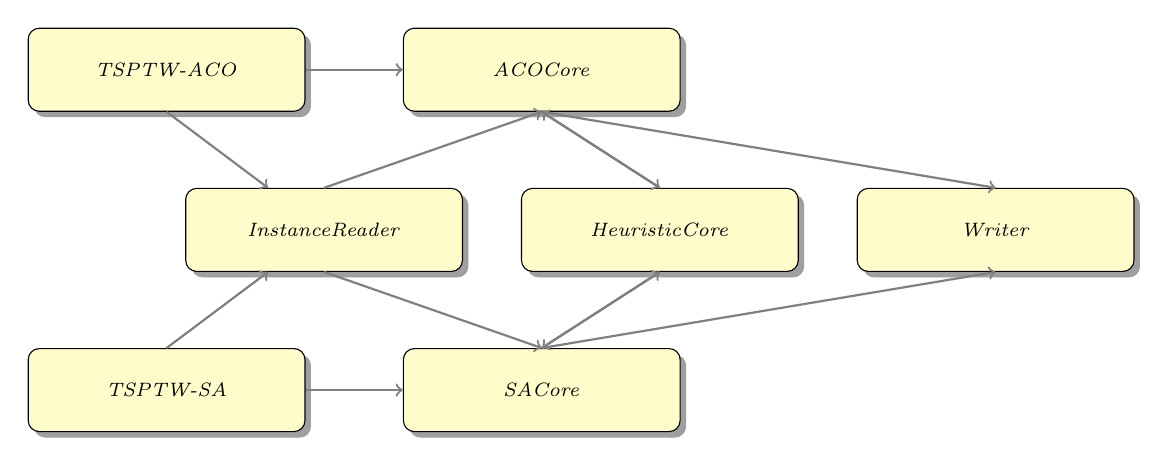
\begin{tikzpicture}[transform shape]
 
  % Draw diagram elements
  
  \path \component {1}{InstanceReader};
  \path (p1.north)+(-2.0,+1.5) \component{3}{TSPTW-ACO};
  \path (p1.south)+(-2.0,-1.5) \component{4}{TSPTW-SA};
  \path (p3.east)+(+3.0,0.0) \component{5}{ACOCore};
  \path (p4.east)+(+3.0,0.0) \component{6}{SACore};
  \path (p1.east)+(+2.5,0.0) \component{7}{HeuristicCore};
  \path (p7.east)+(+2.5,+0.0) \component {2}{Writer};
     
  % Draw arrows between elements
  \path [line] (p3.south) -> node [above] {} (p1);
  \path [line] (p4.north) -> node [above] {} (p1);
  \path [line] (p1.north) -> node [above, midway] {} (p5.south);
  \path [line] (p1.south) -> node [above, midway] {} (p6.north);
  \path [line] (p3.east) -> node [above] {} (p5.west);
  \path [line] (p4.east) -> node [above] {} (p6.west);
  \path [line] (p5.south) -> node [above] {} (p2.north);
  \path [line] (p6.north) -> node [above] {} (p2.south);
  \path [line] (p5.south) -> node [above] {} (p7.north);
  \path [line] (p6.north) -> node [above] {} (p7.south);
  \path [line] (p7.south) -> node [above] {} (p6.north);
  \path [line] (p7.north) -> node [above] {} (p5.south);
  %\backgroundSquare{p1}{p1}{p3}{p3}{Presentation}

 \end{tikzpicture}
 \captionof{figure}{Simulation Code Structure}
\end{center}

The names of the nodes corresponds to those of the implementation (.cpp) and header files for the corresponding classes.

In addition to these, a class to represent the time windows (TimeWindow.h), one to represent the candidate solution as
a user defined data type (CandidateSolution.\{h,cpp\}) and one to implement the virtual ant (Ant.h) have been implemented.

In order to improve the performances of the algorithm a template class called \emph{NumericMatrix} has been created to reduce the computation time due to the access to the matrices (distance and pheromone).

\subsection{How to compile the program?}
The software was developed in C++98 under Linux (Debian Wheezy), using the GNU g++ (Debian 4.7.2-5) 4.7.2 compiler and tested in this environment. 
The software is distributed as a compressed tar file, containing both the source code (in the \verb|src| folder) and the scripts and instances (in the \verb|bin| and \verb|bin\instances| respectively).
To install the program, first obtain the file TSPTW.V1.1.tar.gz. 

Unzip the file by typing:

\begin{center}
\begin{verbatim}
gunzip TSPTW.V1.1.tar.gz
\end{verbatim}
\end{center}

and then unpack it by typing:

\begin{center}
\begin{verbatim}
tar -xvf TSPTW.V1.1.tar
\end{verbatim}
\end{center}

The software will be extracted in a new folder TSPTW.V1.0 

Finally, by launching
\begin{center}
\begin{verbatim}
make all
\end{verbatim}
\end{center}

the Makefile will trigger the compilation of the files,
producing the executables 'TSPTW-II','TSPTW-VND','TSPTW-ACO','TSPTW-SA' in the \verb|bin| folder.

\textbf{Note:} The code is written in C++98. Hence, the code should be
reasonably portable to other Operating Systems than Linux or Unix.

\subsection{How to run the program?}

Once the program has been compiled, two separate executable files,
corresponding to the different kind of metaheuristic (i.e. Iterative Improvement
and Variable Neighborhood Descent) can be either launched directly via the command line
interface or using the bash script to launch.

The design choice to separate the two different kind of metaheuristic is made in order to limit the number of command line parameters to be given as input to the program.

\subsubsection{Command-line execution}
By launching\footnote{The squared-bracket notation implies that the formal parameters to the script have to be substituted by their actual value.}:
\begin{center}
\begin{verbatim}
./TSPTW-ACO [PARAMETERS] -i [INPUT_FILE] -s [SEEDS_FILE]
\end{verbatim}
\begin{verbatim}
./TSPTW-SA [PARAMETERS] -i [INPUT_FILE] -s [SEEDS_FILE]
\end{verbatim}
\end{center}

one can display the information about the meaning of the different options that can be given as input to the program.

Additional information concerning the usage of the program can be found in the README file.

The only mandatory options are "-i, --input" and "-s,-seeds", since
without these components will not be possible to execute the simulation.

The argument to the input option must contain the full path to the instance file.

The seeds file must contain a number of seeds at least equal to the number of
runs required, one seed per line without any additional information.

The options controlling the same parameters are mutually exclusive, with that
meaning that only one option must be selected in order to run the program.
If multiple options for the same parameter are chosen, the program will not
run.

\paragraph{TSPTW-II}
\begin{tabular}{|l|c|}
\hline
\textbf{Parameter}	&	\textbf{Mutually exclusive options} \\ \hline
Initial solution & -d,--random , -h,--heuristic \\ \hline
Neighborhood type &-t,--transpose , -e,--exchange , -n,--insert \\ \hline 
Pivoting rule &	-f,--first-imp , -b,--best-imp \\ \hline
\end{tabular}

\paragraph{TSPTW-VND}

\begin{tabular}{|l|c|}
\hline
\textbf{Parameter}	&	\textbf{Mutually exclusive options} \\ \hline
VND algorithm & -t,--standard , -p,--piped \\ \hline
Neighborhood chain & 	-a,--TEI  , -b,--TIE \\ \hline
\end{tabular}

\paragraph{Output}
Every experiment produces a single file:
\begin{itemize}
  \item \textbf{(II)} $[pivoting\_rule].[neighborhood\_type].[INSTANCE\_NAME]$ with $[pivoting\_rule] \in \{first,best\}$ and $[neighborhood\_type] \in \{transpose,exchange,insert\}$ 
  \item \textbf{(VND)} $[vnd\_type].[neighborhood\_chain].[INSTANCE\_NAME]$ with $[vnd\_type] \in \{standard,piped\}$ and $[neighborhood\_type] \in \{tei,tie\}$
\end{itemize} 
				
					 
\textbf{Examples:} \begin{verbatim}
ACO.n80w200.004.txt
SA.n80w20.003.txt
\end{verbatim}


The internal structure of the file is the following: 
\begin{tabular}{|c|c|c|c|}
\hline
\textbf{Seed}	&	\textbf{CV} & \textbf{PRPD} \\ \hline
\end{tabular}

For each run of the algorithm, the program writes in the file, using a tabulation as separator,
the used seed, the number of constraints violations and the penalised relative percentage deviation.


\subsubsection{Script execution}
By launching:
\begin{center}
\begin{verbatim}
./launchTSPTW-II.sh [INSTANCE_NAME] [RUNS] [SEEDS_FILE]
\end{verbatim}
\begin{verbatim}
./launchTSPTW-VND.sh [INSTANCE_NAME] [RUNS] [SEEDS_FILE]
\end{verbatim}
\end{center}

The script will:
\begin{enumerate}
  \item Create the files required by the data processing script to write statistics.
  \item Generate a seed file, named [SEEDS\_FILE] containing [RUNS] randomly generated seeds.
  \item Launch the corresponding TSPTW program for [RUNS]  using all the possible combinations of input options.
  \item Wait for the termination of all the previously launched experiment and call the R data processing script
\end{enumerate}

The script assumes that all the instances are located into the instances folder, hence it is only necessary to indicate the instance name, instead of the complete path.

\paragraph{Output}

Each execution of the script will then generate the files:
\begin{itemize}
  \item $[INSTANCE\_NAME]-CpuTime.pdf$ containing the boxplots of the runtime distribution for each algorithm.
  \item $[INSTANCE\_NAME]-PRPD.pdf$ containing the boxplots of the PRPD distribution for each algorithm.
  \item 
        \begin{itemize}
          \item \textbf{(II)} transpose.first, exchange.first, insert.first, transpose.best, exchange.best, insert.best 
          \item \textbf{(VND)} standard.tei, standard.tie, piped.tei, piped.tie
        \end{itemize}
\end{itemize}

The internal structure of the file is the following:
 
\begin{tabular}{|c|c|c|c|}
\hline
\textbf{Instance}	&	\textbf{Infeasible} & \textbf{mean(PRDP)} &	\textbf{mean(CpuTime)} \\ \hline
\end{tabular}

Each line contains the instance name, the percentage of infeasible runs, the mean PRDP and the mean runtime across [RUNS] runs.

\section{Problem formulation}
An instance of the Travelling Salesman Problem with Time Windows (TSPTW) can be expressed as a tuple $<N,E,c,t>$ where:
\begin{itemize}
  \item $N:\{0,\cdots,n\}$ - Node set 
  \item $E:N\times N$ - Edge set
  \item $c:E\mapsto \mathbb{R}$ - Edge cost function mapping a cost $c$ to every edge $e \in E$. 
  \item $t:N\mapsto \mathbb{R}^2$ - Time window function mapping a couple of values $a_i,b_i$ representing respectively, the opening and closing time of the time window, such that $a_i<b_i$, to every node $i \in N$.
  \item A candidate solution for the problem, in this case, is represented as a permutation $p$ of the nodes in $N$, where $p_i$ represents the $i^{th}$ solution component (node) in the sequence, such that $p_0 = 0 \forall p$.
\end{itemize}

As in \cite{lopez2010beam} the formal definition of the problem is:
\begin{equation} \label{eq:probform}
 \begin{array}{rl}
  \textbf{min} & f(p)= \sum\limits_{i=0}^{n} c(e_{p_{i}p_{k+i}}) \\
  \textbf{subject to} & \Omega(p)= \sum\limits_{i=0}^{n+1} \omega(p_{i}) = 0
 \end{array}
\end{equation}

where

\begin{equation} \label{eq:cv}
\begin{array}{c}
 \omega(p_{i}) \begin{cases}
                1 & A_{p_i} < b_{p_i}  \\
                0 & \text{otherwise} \\   
               \end{cases} \\
 A_{p_{i+1}} = \max(A_{p_i},a_i) + c(e_{p_{i}p_{k+i}}) 
\end{array}
\end{equation}

As one may notice in \ref{eq:probform} and \ref{eq:cv}, a feasible solution $p$ for the problem is a permutation where the constraints related to the time windows are met for every node $i$ in the permutation.


%----------------------------------------------------------------------------------------
%	PROBLEM 1
%----------------------------------------------------------------------------------------

% To have just one problem per page, simply put a \clearpage after each problem
\newpage
\begin{homeworkProblem}
\section{Ant Colony Optimization} \label{aco}
\subsection{Problem statement}
Implement two stochastic local search (SLS) algorithms for the traveling salesman problem with time windows (TPSTW), building on top of the perturbative local search methods from the first implementation exercise.
\begin{enumerate}
  \item Run each algorithm 25 times with different random seed on each instance. Instances will be available from http://iridia.ulb.ac.be/˜stuetzle/Teaching/HO/. As termination criterion, for each instance, use the maximum computation time it takes to run a full VND (implemented in the previous exercise) on the same instance and then multiply this time by 1000 (to allow for long enough runs of the SLS algorithms).
 \item Compute the following statistics for each of the two SLS algorithms and each instance:
 \begin{itemize}
   \item Percentage of runs with constraint violations
   \item Mean penalized relative percentage deviation
 \end{itemize}

\item Produce box-plots of penalized relative percentage deviation.
\item Determine, using statistical tests (in this case, the Wilcoxon test), whether there is a statistically significant difference between the quality of the solutions generated by the two algorithms.
\item Measure, for each of the implemented algorithms on 5 instances, the run-time distributions to reach sufficiently high quality solutions (e.g. best-known solutions available at http://iridia.ulb.ac.be/˜manuel/tsptw-instances\#instances).
Measure the run-time distributions across 25 repetitions using a cut-off time of 10 times the termination criterion above.
\item Produce a written report on the implementation exercise:
\begin{itemize}
  \item Please make sure that each implemented SLS algorithm is appropriately described and that the computational results are carefully interpreted. Justify also the choice of the parameter settings and the choice
of the iterative improvement algorithm for the hybrid SLS algorithm.
  \item Present the results as in the previous implementation exercise (tables, box-plots, statistical tests).
  \item Present graphically the results of the analysis of the run-time distributions.
  \item Interpret appropriately the results and make conclusions on the relative performance of the algorithms across all the benchmark instances studied.
\end{itemize}
\end{enumerate}

\subsection{Introduction} \label{sec:introACO}
Ant Colony Optimization is an example of population-based metaheuristic (i.e a set of algorithmic concepts that can be used to define heuristic methods) inspired by the behavior of the ant species \emph{Iridomyrmex humilis}.

To be more precise, these insects are able, by means of stigmergic communication, to choose the shortest path between their nest and a food source, when given the choice (\cite{deneubourg1990self}).

The communication process occurs by deposing a certain quantity of pheromone in the environment that can be sensed by the other ants and that will be used by them as an heuristic (i.e an information to guide their choice) for selecting the shortest path.

Furthermore, the pheromone quantity on a certain location decreases over time because of evaporation, thus requiring a continuous deposit process to be effective.

The convergence to one of the paths will occur as a consequence of the self-reinforcing pheromone deposit mechanism.
In fact the more pheromone is deposited on a path, the more ants will follow the pheromone trail on that path deposing even more pheromone.

The first application of Ant Colony Optimization method, the Ant System, has been made on the optimization version of the Travelling Salesman Problem (TSP) (\cite{dorigo1996ant}).

In this implementation a population of virtual agents (an ant colony) is used to explore the search space (the virtual environment).

In the same fashion as the real insects, the ants are able to deposit virtual pheromone in the environment, to signal to the other ants the presence of promising solutions.

The general outline of the implemented algorithm is the following: 

\begin{algorithm}[!h]
  \caption{Ant Colony Optimization - Outline}\label{aco}
  \begin{algorithmic}[1]
    \State \emph{InitalizePheromoneTrail} 
    \While{!(TerminationCondition)}
        \State \emph{ConstructAntsSolutions}
        \State \emph{LocalSearch} (Optional)
        \State \emph{UpdatePheromoneTrails}
    \EndWhile
\end{algorithmic}
\end{algorithm}

The design of the solution construction and pheromone update mechanism is the main point of the algorithm.
Implementation details of the basic ACO system, the Ant System can be found in \cite{dorigo2006artificial}.

\subsection{Algorithm structure} \label{sec:algstrucACO}
The proposed algorithm is an implementation of one of the extensions to the Ant Colony Optimization metaheuristic framework, the \maxmin Ant System (cf. \cite{stutzle2000max}).
The main differences with respect to the basic ACO approach are the following:
\begin{itemize}
  \item Only iteration best or best-so-far ants update pheromone.
  \item A local search after the solution generation is used to further improve the solutions found by the ants at each iteration.
  \item $\forall t \text{ } \tau_{\min} < \tau_{i,j}(t) < \tau_{\max}  $ - Pheromone trails have explicit upper and lower limits
  \item Pheromone trails are re-initialized when stagnated.
\end{itemize}

The aforementioned design choice were made because:

\begin{itemize}
    \item The initialization of the pheromone trails to their upper bound favors diversification at the beginning of each trial.
    \item The pheromone update rule favors exploitation of (intensification on) the best solutions at each iteration of the algorithm.
    \item By bounding the intensity of the pheromone trails, the probability of stagnation (i.e. all the ants converging and exploiting a single sub-optimal tour) is reduced.
    \item If the pheromone trails values for the solution components of a certain tour $s$ are equal to $\tau_{\max}$, the algorithm is said to be converged.
  \end{itemize}
  

\begin{algorithm}[!h]
  \caption{\maxmin Ant System for TSPTW - Outline}\label{maxmintsptw}
  \begin{algorithmic}[1]
    \Procedure{ACO}{$\alpha,\beta,\rho,\tau_0,p_b,t_{\max},f_{best}$}\Comment{The main procedure}
    \Require $N$ - Node set
    \Require $E$ - Edge set 
    \Require $c$ - Edge cost function
    \Require $t$ - Time window function
    \State {\emph{InitalizePheromoneTrail}($\tau_0,n_{cities}$)}
    \While{\emph{!TerminationCondition}($s,t_{max},f_{best}$)}
      \ForAll {Ant $k$}
        \State $s' \gets$ \emph{ConstructSolution}($\alpha,\beta$)
        \If {\emph{IsImproved}($s,s'$)}
          \State $s \gets s' $
        \EndIf 
      \EndFor
      \State $s \gets$\emph{IterativeImprovementIBI}()
      \State \emph{UpdatePheromoneTrails}($\rho,\varepsilon$)
    \EndWhile
    \State \textbf{return} $s$
    \State
  \EndProcedure
\end{algorithmic}
\end{algorithm}

\begin{center}
  
\begin{minipage}{.45\textwidth}
\centering
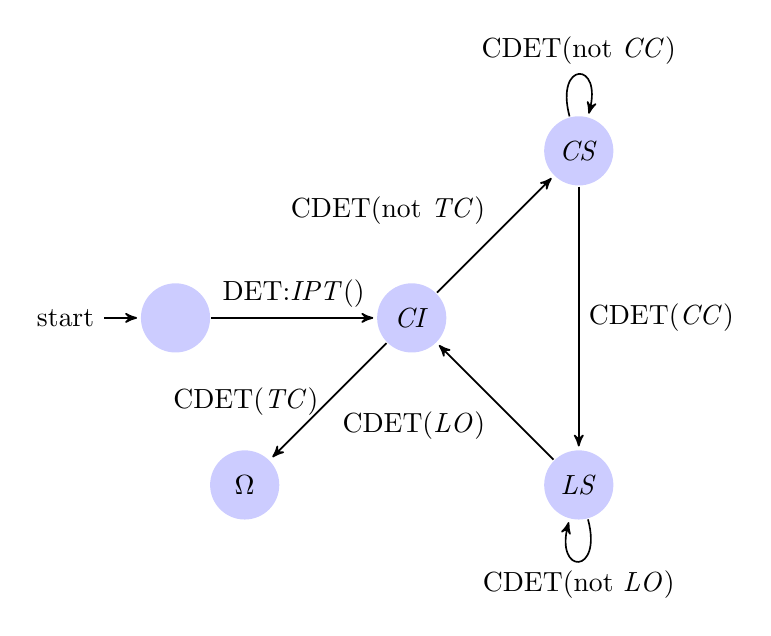
\begin{tikzpicture}[->,>=stealth',shorten >=1pt,auto,node distance=3cm,
                    semithick]
  \tikzstyle{every state}=[fill=blue!20,draw=none,thick]

  \node[initial,state]    (Init)                   {};
  \node[state]            (CI) [right of=Init]     {\emph{CI}};
  \node[state]            (CS) [above right of=CI] {\emph{CS}};
  \node[state]            (LS) [below right of=CI] {\emph{LS}};
  \node[state,accepting]  (End)[below left of=CI]  {$\Omega$};

  \path (Init) edge              node {DET:\emph{IPT}()} (CI)
        (CI) edge              node {CDET(not \emph{TC})} (CS)
             edge [left]       node {CDET(\emph{TC})} (End)
        (CS) edge [loop above] node {CDET(not \emph{CC})} (CS)
            edge              node {CDET(\emph{CC})} (LS)
        (LS) edge [loop below] node {CDET(not \emph{LO})} (LS)
            edge               node {CDET(\emph{LO})} (CI);
\end{tikzpicture}
\end{minipage}%
\hspace{1.5cm}
\begin{minipage}{.45\textwidth}
\centering
\paragraph{Nodes}
\begin{itemize}
  \item \emph{CI} $\equiv$ Dummy node
  \item \emph{CS} $\equiv$ \emph{ConstructSolution}($\alpha,\beta$)
  \item \emph{LS} $\equiv$ \emph{IterativeImprovementIBI}()
\end{itemize}
\paragraph{Conditions}
\begin{itemize}
  \item \emph{IPT} $\equiv$ \emph{InitializePheromoneTrail}()
  \item \emph{CC} $\equiv$ \emph{ConstructionComplete}()
  \item \emph{LO} $\equiv$ \emph{LocalOptimum}()
  \item \emph{TC} $\equiv$ \emph{TerminationCondition}($s,t_{max},f_{best}$)
\end{itemize}
\end{minipage}
\captionof{figure}{\maxmin  Ant System GLSM}
\end{center}

\newpage
In the implementation, an instance is completely defined by:
\begin{itemize}
\item \textbf{Cost matrix} - Encapsulating information on the node set $N$, edge set $E$, and weighting of each edge $c$.
\item \textbf{Time window vector} - Describing the time window mapping function $t$ for each node.
\end{itemize}

\subsubsection{Pheromone Initialization}
\begin{algorithm}[!h]
  \caption{Pheromone Initialization}\label{init}
  \begin{algorithmic}[1]
    \Procedure{InitalizePheromoneTrail}{$\tau_0,n_{cities}$}
      \State $\tau_{\max} \gets $
      \State $\tau_{\min} \gets $
      \State $i \gets 0$
      \State $j \gets 0$
      \For{$i < n_{cities}$} 
        \For{$j < i$} 
          \State $\tau_{ij} \gets \tau_0$
          \State $\tau_{ji} \gets \tau_{ij}$
          \State $ j \gets j + 1$  
        \EndFor
        \State $ i \gets i + 1$ 
      \EndFor
    \EndProcedure
\end{algorithmic}
\end{algorithm}

As discussed in \nameref{sec:introACO}, the ACO methods are based on stigmergic communication among the agents by means of virtual pheromone.

While the real ants can deposit pheromone anywhere in the environment, the virtual ants may only exchange information concerning solutions components.

For this reason, every admissible edge $e_{i,j}$ of $E$ has an associated pheromone value $\tau_{i,j}$, that have to be initialized at the beginning of the execution of the algorithm.

The initialization value $\tau_0$ is a parameter of the algorithm, for the \maxmin Ant System $\tau_0 = \tau_{i,j}(0) = \tau_{\max}$. 


\subsubsection{Solution construction}
\begin{algorithm}[!h]
  \caption{Solution Construction}\label{sol}
  \begin{algorithmic}[1]
    \Procedure{ConstructSolution}{$\alpha,\beta$}\Comment{The main procedure}
      \State \Comment{$s_i$ reprents the $i^{th}$ component of the solution}
      \State $s_0 \gets 0$ \Comment{Every solution starts at the depot}
      \State $s_1 \gets$ \emph{RandomCitySelection}() \Comment{Random choice of the starting city}
      \State $i \gets 1$
      \While{!\emph{SolutionComplete}()}
        \State $s_i \gets $ \emph{RouletteWheelSelection}() \Comment{ $s_i$ stochastically chosen according to the probability distribution defined by \ref{eq:tranprob}} 
        \State $i \gets i+1$
      \EndWhile
    \EndProcedure
\end{algorithmic}
\end{algorithm}

The solution construction process, used by every ant $k$ in the system, consist of a probabilistic selection of solution components.
Every edge $e_{i,j}$ has a selection probability $p_{i,j}^k(t)$ (also called transition probability) defined as follows:

\begin{equation} \label{eq:tranprob}
p_{i,j}^k(t) = \begin{cases}
  \frac{[\tau_{i,j}(t)]^\alpha \cdot [\eta_{i,j}]^\beta}{\sum_{k} \in A(s_{i}) [\tau_{k,j}(t)]^\alpha \cdot [\eta_{k,j}]^\beta} & j \in A(s_{i}) \\
 0 & \text{otherwise} \\
\end{cases}
\end{equation}

As one can see in \ref{eq:tranprob}, the transition probability is determined by a constant, locally available heuristic information $\eta_{i,j}$ and by the time varying pheromone trail $\tau_{i,j}(t)$.
This probability is defined on the set $A(s_i)$ of available (i.e. not yet visited) cities while visiting solution component $s_i$.
The value of the parameters $\alpha$ and $\beta$ determines the relative importance of the heuristic information and the pheromone trail, respectively.

\subsubsection{Solution improvement}
\begin{algorithm}[!h]
  \caption{Solution improvement}\label{sol}
  \begin{algorithmic}[1]
    \Procedure{IsImproving}{$s,s'$}\Comment{The main procedure}
      \If {$\Omega(s') < \Omega(s)$}
          \State \textbf{return true}
      \Else
           \If {$\Omega(s') = \Omega(s) \wedge f(s') < f(s)$}
            \State \textbf{return true}
           \EndIf
      \EndIf
      \State \textbf{return false}
      \EndProcedure
\end{algorithmic}
\end{algorithm}

A solution $s'$ is considered improving the current best solution $s$ if and only if:
\begin{itemize}
  \item Either,it has a smaller number of constraints violation (i.e. $\Omega(s') < \Omega(s)$)
  \item Or, it has the same number of constraints violations ($\Omega(s') == \Omega(s)$) but the total tour duration is smaller ($f(s') < f(s)$).
\end{itemize}


\subsubsection{Admissible heuristics}
The heuristic component $\eta_{i,j}$ is used to guide the selection of solution components towards those components that are included in optimal solution.

\paragraph{Dorigo et al, 1996}
The heuristic originally proposed by Dorigo et al, in \cite{dorigo1996ant}, for the TSP problem is:
\begin{equation}
  \eta_{i,j} = \frac{1}{c(e_{i,j})}
\end{equation}

The main idea behind this heuristic is that, if the selection process tends to select, at each step, the shortest connection between the current node and the following, the built tour should be of the shortest length.
This heuristic is cited for explanation purposes, even though it cannot be used for the TSPTW problem, since it will guide the exploration only towards shorter solutions, without taking into account the presence of the time windows.

\paragraph{Cheng and Mao, 2007}
The local heuristics used in \cite{cheng2007modified} are similar to that proposed by Gambardella et al. \cite{gambardella1999macs} in their multiple ant colony system (MACS) designed to solve the vehicle routing problem with time windows (VRPTW).

\begin{equation}
[\eta_{i,j}]^\beta = [g_{i,j}]^\beta \cdot [h_{i,j}]^\gamma
\end{equation}  

The two components $g_{i,j}$ and $h_{i,j}$, are designed, respectively, to avoid lateness (that is, arriving in the node where the time windows is already terminated) and waiting times (i.e. arriving in the node before the time windows open).

\subparagraph{Lateness avoidance}
\begin{equation}
g_{i,j} = \begin{cases}
 \frac{1}{1+e^{\delta \cdot (G_{i,j} - \mu)}}  &  G_{i,j} = b_j - t_j \geq 0 \\
0 & \text{otherwise} \\
\end{cases}
\end{equation}
where
\begin{itemize}
  \item $G_{i,j} = b_j - t_j$ - Slack corresponding to the time window $j$ while being in node $i$
  \item $t_i$ - Arrival time at node $i$
  \item $b_i$ - Closing time of time window $i$
  \item $G(i) = \{k\text{ } | \text{ }G_{i,k} \geq 0\}$ - Set of feasible neighbors of node $i$ (i.e. such that node $k$ is reached earlier than its closing time)
  \item $\mu = \frac{1}{|G(i)|}\sum_{j \in G(i)}  G_{i,j}$ - Average slack 
  \item $\delta$ - Parameter to control the slope of the sigmoidal function
\end{itemize}

\subparagraph{Waiting time avoidance}
\begin{equation}
h_{i,j} = \begin{cases}
 \frac{1}{1+e^{\lambda \cdot (H_{i,j} - \upsilon)}}  &  H_{i,j} = t_j - a_j \geq 0 \\
0 & \text{otherwise} \\
\end{cases}
\end{equation}
where
\begin{itemize}
  \item $H_{i,j} = t_j - a_j$ - Waiting time corresponding to the time window $j$ while being in node $i$
  \item $t_i$ - Arrival time at node $i$
  \item $a_i$ - Opening time of time window $i$
  \item $H(i) = \{k\text{ } | \text{ }H_{i,k} \geq 0\}$ - Set of non-waiting neighbors of node $i$ (i.e such that node $k$ is reached within the time window)
  \item $\upsilon = \frac{1}{|H(i)|}\sum_{j \in H(i)}  H_{i,j}$ - Average waiting time 
  $\lambda$ - Parameter to control the slope of the sigmoidal function 
\end{itemize}


\paragraph{Lopez-Ibanez and Blum, 2010}
The approach used in \cite{lopez2010beam} is a linear combination based on $\lambda_i$ coefficients, of the normalized values of opening and closing times of the time windows and the travelling cost from one city to another.

\begin{equation} \label{eq:heuristic}
\eta_{i-1,k} = \lambda_{a} \cdot \frac{a_{\max}-a_{k}}{a_{\max}-a_{\min}} + \lambda_{b} \cdot \frac{b_{\max}-b_{k}}{b_{\max}-b_{\min}} + \lambda_{c} \cdot \frac{c_{\max}-c_{i-1,k}}{c_{\max}-c_{\min}}
\end{equation}

where
\begin{itemize}
  \item $a_i$ - Opening time of time window $i$
  \item $a_{\max} = \max_{j \in N} a_{j}$ - Maximum time window opening time in the neighborhood of node $i$
  \item $a_{\min} = \min_{j \in N} a_{j}$ - Minimum time window opening time in the neighborhood of node $i$
  \item $b_i$ - Closing time of time window $i$
  \item $b_{\max} = \max_{j \in N} b_{j}$ - Maximum time window closing time in the neighborhood of node $i$
  \item $b_{\min} = \min_{j \in N} b_{j}$ - Minimum time window closing time in the neighborhood of node $i$
  \item $c_{i,j}$ - Travelling cost from node $i$ to node $j$
  \item $c_{\max} = \max_j c_{i,j}$ - Maximum travelling cost from node $i$ 
  \item $c_{\min} = \min_j c_{i,j}$ - Minimum travelling cost from node $i$
  \item $\lambda_{a},\lambda_{b},\lambda_{c}$ s.t. $\lambda_{a}+\lambda_{b}+\lambda_{c}=1$ - Randomly selected weights
\end{itemize}

In this implementation, the heuristic information will be computed according to \cite{lopez2010beam}

\subsubsection{Pheromone trails update}
\begin{algorithm}[!h]
  \caption{Pheromone Trails Update}\label{update}
  \begin{algorithmic}[1]
    \Procedure{UpdatePheromoneTrails}{$\rho,p_b$}\Comment{The main procedure}
     \State $i \gets 0$
      \State $j \gets 0$
      \For{$i < n_{cities}$} 
        \For{$j < i$}
          \If{\emph{Random}() $< \varepsilon$} 
          \State $\tau_{ij} \gets (1-\rho)\cdot\tau_{ij}+\Delta\tau_{i,j}^{Bi}$
          \Else
          \State $\tau_{ij} \gets (1-\rho)\cdot\tau_{ij}+\Delta\tau_{i,j}^{Bo}$
          \EndIf
          \If{$\tau_{ij} < \tau_{\min}$} 
            \State $\tau_{ij} \gets \tau_{\min}$
          \EndIf
          \If{$\tau_{ij} > \tau_{\max}$} 
            \State $\tau_{ij} \gets \tau_{\max}$
          \EndIf
          \State $\tau_{ji} \gets \tau_{ij}$
          \State $ j \gets j + 1$  
        \EndFor
        \State $ i \gets i + 1$ 
      \EndFor
    \EndProcedure
\end{algorithmic}
\end{algorithm}

As discussed in \nameref{sec:algstrucACO}, the pheromone update will be made by a single ant, being either the one who found the best solution in the current iteration: 

\begin{equation}
  \Delta\tau_{i,j}^{Bi} = \begin{cases}
    \frac{1}{T_{d}^{\text{Bi}}} & e_{i,j} \in T^{\text{Bi}}  \\
    0 & \text{otherwise} 
      \end{cases}
\end{equation}

Or the one having found the global best (best-so-far) solution:

\begin{equation}
  \Delta\tau_{i,j}^{Bo} = \begin{cases}
    \frac{1}{T_{d}^{\text{Bo}}} & e_{i,j} \in T^{\text{Bo}}  \\
    0 & \text{otherwise} 
  \end{cases}
\end{equation}

where
\begin{itemize}
\item $e_{i,j}$ - Edge connecting node $i$ and $j$
\item $T_{d}^{i}$ - Complete tour duration of tour $i$
\item $T^{\text{Bi}}$ - Best tour of the current iteration
\item $T^{\text{Bo}}$ - Best tour overall 
\end{itemize}


Provided that the best solution is known, the bounds on the pheromone values can be estimated by:
\begin{equation}
\begin{array}{lccr}
  \hat{\tau}_{\max} = \frac{1}{\rho \cdot T_{d}^{\text{Go}}} & & & \hat{\tau}_{\min} = \frac{\hat{\tau}_{\max}}{a}
\end{array}
\end{equation}

\subsubsection{Local search}
\begin{algorithm}[!h]
  \caption{Iterative Improvement - (Insert neighborhood with best improve pivoting rule)}\label{locsearch}
  \begin{algorithmic}[1]
    \Procedure{IterativeImprovementIBI}{$s$}\Comment{The main procedure}
      \State $s^{*} \gets s$ 
      \For {$i \in \{1,\cdots,|N|\}$}
        \For {$j \in \{1,\cdots,|N|\}$}
          \If{ $i = j \vee  j = i-1 $}
				    \State \textbf{continue}
			    \EndIf
			    \State $s' \gets$ \emph{InsertTourComponent}($s,i,j$)
			    \If {\emph{IsImproving}($s^{*},s'$)}
          \State $s^{*} \gets s'$
        \EndIf
        \EndFor
      \EndFor
      \State \textbf{return} $s^{*}$
    \EndProcedure
\end{algorithmic}
\end{algorithm}

\begin{algorithm}[!h]
  \caption{Insert neighbor solution computation}\label{locsearch}
  \begin{algorithmic}[1]
    \Procedure{InsertTourComponent}{$s,i,j$}\Comment{The main procedure}
      \State \Comment{$s_i$ reprents the $i^{th}$ component of the solution}
      \State $e \gets s_i$
      \If{i<j}
      \State $k \gets i$
        \While{$k < j$}
				  \State $s_i \gets s_{i+1}$
				  \State $k \gets k+1$
			  \EndWhile
			\Else
			\State $k \gets i$
        \While{$k > j$}
				  \State $s_i \gets s_{i-1}$
				  \State $k \gets k-1$
			  \EndWhile
			\EndIf
			\State $s_j \gets e$
     \State \textbf{return} $s$
    \EndProcedure
\end{algorithmic}
\end{algorithm}


The solution construction process, used by every ant $k$ in the system, consist of a probabilistic selection of solution components.
Every edge $e_{i,j}$ has a selection probability $p_{i,j}^k(t)$ (also called transition probability) defined as follows:

\begin{equation} 
p_{i,j}^k(t) = \begin{cases}
  \frac{[\tau_{i,j}(t)]^\alpha \cdot [\eta_{i,j}]^\beta}{\sum_{k} \in A(s_{i}) [\tau_{k,j}(t)]^\alpha \cdot [\eta_{k,j}]^\beta} & j \in A(s_{i}) \\
 0 & \text{otherwise} \\
\end{cases}
\end{equation}

As one can see in \ref{eq:tranprob}, the transition probability is determined by a constant, locally available heuristic information $\eta_{i,j}$ and by the time varying pheromone trail $\tau_{i,j}(t)$.
This probability is defined on the set $A(s_i)$ of available (i.e. not yet visited) cities while visiting solution component $s_i$.
The value of the parameters $\alpha$ and $\beta$ determines the relative importance of the heuristic information and the pheromone trail, respectively.

\subsubsection{Termination condition}
\begin{algorithm}[!h]
  \caption{Termination Condition}\label{termcond}
  \begin{algorithmic}[1]
    \Procedure{TerminationCondintion}{$s,t_{\max},s_{best}$}
          \If{ $(f(s) = f_{best} \wedge \Omega(s) = 0) \vee  t > t_{\max} $}
				    \State \textbf{return true}
			    \EndIf
      \State \textbf{return false}
    \EndProcedure
\end{algorithmic}
\end{algorithm}

\subsubsection{Implementation parameters}
\begin{center}
\begin{tabular}{|c|c|c|}
\hline
\textbf{Parameter} & \textbf{Default} & \textbf{Selected} \\ \hline 
$\alpha$ & 1.0 & 1.0 \\\hline
$\beta$ & 2.0 & 2.0 \\\hline 
$\tau_0$ & 1.0 & 1.0 \\ \hline
$\varepsilon$ & 0.5 & 0.5 \\ \hline 
$Ants$ & 25 & 25 \\ \hline  
$t_{\max}$ & 10[s] & 10[s] \\ \hline
\end{tabular}
\captionof{table}{SA - Algorithm parameters overview}
\label{saParameters}
\end{center}

 
\end{homeworkProblem}

%----------------------------------------------------------------------------------------
%	PROBLEM 1
%----------------------------------------------------------------------------------------

% To have just one problem per page, simply put a \clearpage after each problem
\newpage
\begin{homeworkProblem}
\section{Simulated Annealing}
\subsection{Problem statement}
Implement two stochastic local search (SLS) algorithms for the traveling salesman problem with time windows (TPSTW), building on top of the perturbative local search methods from the first implementation exercise.
\begin{enumerate}
  \item Run each algorithm 25 times with different random seed on each instance. Instances will be available from http://iridia.ulb.ac.be/˜stuetzle/Teaching/HO/. As termination criterion, for each instance, use the maximum computation time it takes to run a full VND (implemented in the previous exercise) on the same instance and then multiply this time by 1000 (to allow for long enough runs of the SLS algorithms).
 \item Compute the following statistics for each of the two SLS algorithms and each instance:
 \begin{itemize}
   \item Percentage of runs with constraint violations
   \item Mean penalised relative percentage deviation
 \end{itemize}

\item Produce boxplots of penalised relative percentage deviation.
\item Determine, using statistical tests (in this case, the Wilcoxon test), whether there is a statistically significant difference between the quality of the solutions generated by the two algorithms.
\item Measure, for each of the implemented algorithms on 5 instances, the run-time distributions to reach sufficiently high quality solutions (e.g. best-known solutions available at http://iridia.ulb.ac.be/˜manuel/tsptw-instances\#instances).
Measure the run-time distributions across 25 repetitions using a cut-off time of 10 times the termination criterion above.
\item Produce a written report on the implementation exercise:
\begin{itemize}
  \item Please make sure that each implemented SLS algorithm is appropriately described and that the computational results are carefully interpreted. Justify also the choice of the parameter settings and the choice
of the iterative improvement algorithm for the hybrid SLS algorithm.
  \item Present the results as in the previous implementation exercise (tables, boxplots, statistical tests).
  \item Present graphically the results of the analysis of the run-time distributions.
  \item Interpret appropriately the results and make conclusions on the relative performance of the algorithms across all the benchmark instances studied.
\end{itemize}
\end{enumerate}

\subsection{Metric definitions}\label{subsec:metric}
For each algorithm $k$, applied on instance $i$, using different randomly generated seeds one have to compute:
\begin{itemize}
  \item Number of constraint violations
  \item Penalised relative percentage deviation (PRPD)
  \item Computation time (CPU time)
\end{itemize}

In order to perform a statistical analysis of the results, each algorithm $k$ is launched 100 times on the same instance, computing the
following statistics:
\begin{itemize}
  \item Percentage of infeasible solutions (0.x has to be interpreted as x\%) 
  \item Average Penalised relative percentage deviation.
  \item Average Computation time (CPU time).
\end{itemize}

For each instance $i$, the distributions of PRPD and Cpu Times are displayed using box plots and the Wilcoxon signed rank test is performed, in order to assess the existence of a statistically significant difference among the results obtained by the different algorithms on the same instance. 

\paragraph{Constraint Violations}
In the standard formulation of the TSP problem, a solution to the problem is represented by a permutation of the different
entities (solution components), that the hypothetical travelling salesman has to visit.

The best solution for the problem is the permutation that minimizes the total travelling time (distance) among the cities.
The presence of time windows introduce an additional constraint on the feasibility of the solution.

In fact, each solution component has an associated time window within which it has to be visited in order to guarantee the feasiblity of the tour.

Arriving in a (city) before the opening of the corresponding time window involves a delay in the total travelling time (to wait for the time window to open) whereas the arrival after the closure of the time windows will generate a constraint violation.

Thus, a solution is feasible if and only if all the time windows constraints are met, or in other words, if there are no constraint violations.

In this case, the best solution is the feasible solution which minimizes the total travel time.

\paragraph{Penalised Relative Percentage Deviation}
The penalised relative percentage deviation (PRDP from now on) is a measure of the solution quality, with respect to the best known
solution for the instance, taking into account a strong penalisation for the violation of constraints.
The PRPD is computed as follows:
\begin{equation}
pRPD_{kri} = 100 \cdot \frac{(f_{kri} + 10^4\cdot\Omega_{kri})-best_i}{best_i}
\end{equation}

\paragraph{Runtime}
The runtime is a measure of both the quality and the time complexity of the algorithm.

It is measured using the function \verb|int clock_gettime(clockid_t clk_id, struct timespect *tp)| from the \verb|time.h| library.

The parameter \verb|clk_id=CLOCK_PROCESS_CPUTIME_ID|, is used to read the values from an high-resolution timer provided by the CPU for each process.

The runtime is computed (using the user defined function \verb|ComputeRunTime|) as the difference, with a resolution of $10^-9$ s, from the time obtained using \verb|clock_gettime| at the beginning and the one obtained at the end of the simulation.

\subsection{Algorithm structure} \label{sec:algstrucSA}
\begin{algorithm}
\caption{Simulated Annealing TSPTW}
\label{SA:TSPTW}
\begin{algorithmic}
\Procedure{SimulatedAnnealing}{}    
  \Require Annealing schedule
  \State $s \gets$ \emph{InitialSolution}() \Comment{Heuristic or random permutation}
  \State $T \gets T_0$ 
  \While{!\emph{TerminationCondition}()}
    \State $s' \gets$ \emph{ProposalMechanism()} \Comment{(Often) Uniform random choice  in $N(s)$}
    \If{\emph{AcceptanceCriterion}($s,s',T$)} \Comment{(Often) Metropolis condition}
      \State $s \gets s'$
    \EndIf
  \State $T \gets$ \emph{Update}($T$) \Comment{$T_{i+1} = \alpha \cdot T_i$}
\EndWhile
  \State \textbf{return} $s$
\EndProcedure
\end{algorithmic}
\end{algorithm}

\begin{center}
  
\begin{minipage}{.45\textwidth}
\centering
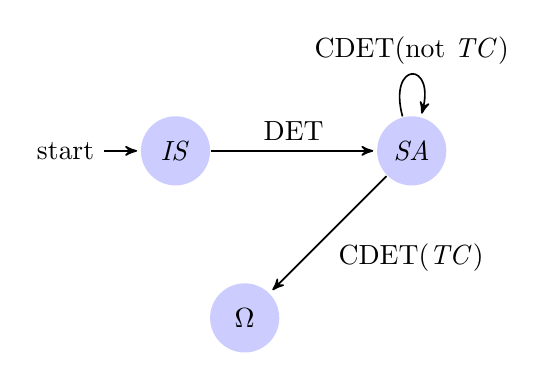
\begin{tikzpicture}[->,>=stealth',shorten >=1pt,auto,node distance=3cm,
                    semithick]
  \tikzstyle{every state}=[fill=blue!20,draw=none,thick]

  \node[initial,state]  (IS)                    {\emph{IS}};
  \node[state]          (SA) [right of=IS]      {\emph{SA}};
  \node[state,accepting](End)[below left of=SA] {$\Omega$};

  \path (IS) edge              node {DET} (SA)
        (SA) edge [loop above] node {CDET(not \emph{TC})} (SA)
             edge              node {CDET(\emph{TC})} (End);
\end{tikzpicture}
\end{minipage}%
\hspace{1.5cm}
\begin{minipage}{.45\textwidth}
\centering
\paragraph{Nodes}
\begin{itemize}
  \item \emph{IS} $\equiv$ \emph{InitialSolution}()
  \item \emph{SA} $\equiv$ \emph{SimulatedAnnealingLoop}
\end{itemize}
\paragraph{Conditions}
\begin{itemize}
  \item \emph{TC} $\equiv$ \emph{TerminationCondition}()
\end{itemize}
\end{minipage}
\captionof{figure}{Simulated Annealing GLSM}
\end{center}



\begin{algorithm}
\caption{Initial solution}
\label{SA:Init}
\begin{algorithmic}
\Procedure{Initial Solution}{}

\State $p \gets$ \emph{UniformRandom}($1,\frac{|N|}{10}$) \Comment{$p$ : Number of perturbations}
\State $s \gets$ \emph{SortCitiesUBTW}() \Comment{Sort cities according upper bound of time window}	

\While{$p > 0$}
  \State $p_p \gets$ \emph{UniformRandom}($1,|N|-1$) \Comment{$p_p$ : Perturbation point}
  \State $p_i \gets$ \emph{UniformRandom}($1,p$) \Comment{$p_i$ : Perturbation intensity}
  \State $s \gets$ \emph{Shuffle}($1+p_p,1+p_p+p_i$) \Comment{Shuffle the solution components occuping the position bounded by the indexes given as parameters}
  \State $p \gets p-1$
\EndWhile	

\State \textbf{return} $s$

\EndProcedure    
\end{algorithmic}
\end{algorithm}

\begin{algorithm}
\caption{Termination condition}
\label{SA:Term}
\begin{algorithmic}
\Procedure{Termination condition}{}
\EndProcedure
\end{algorithmic}
\end{algorithm}

\begin{algorithm}
\caption{Proposal mechanism}
\label{SA:Prop}
\begin{algorithmic}
\Procedure{Proposal mechanism}{} 
  \State $i \gets $ \emph{UniformRandom}($1,|N|$)
  \State $j \gets $ \emph{UniformRandom}($1,|N|$)  
  \State \textbf{return} \emph{InsertTourComponent}($s,i,j$)   
\EndProcedure
\end{algorithmic}
\end{algorithm}

\begin{algorithm}
\caption{Acceptance Criterion}
\label{saTSPTW}
\begin{algorithmic}
\Procedure{Acceptance criterion}{$s,s',T$}
\If {\emph{IsImproved}($s,s',t$)}
  \State \textbf{return} $1$
\Else
  \State \textbf{return} $e^{\frac{f(s)-f(s')}{T}}$
\EndIf
\EndProcedure
\end{algorithmic}
\end{algorithm}

\paragraph{Metropolis condition}
\begin{equation} \label{eq:metropolis}
  P(s,s',T) = \begin{cases}
               1 & f(s) < f(s') \\
               1 & f(s) = f(s') \wedge \Omega(s) < \Omega(s')\\
               e^{\frac{f(s)-f(s')}{T}} & \text{otherwise}
              \end{cases}
\end{equation}

\begin{algorithm}
\caption{Update according to annealing schedule}
\label{saTSPTW}
\begin{algorithmic}
\Procedure{Update}{$T$}
  \State $T \gets \alpha \cdot T$
\EndProcedure
\end{algorithmic}
\end{algorithm}


% \subsection{Experiment results}
% \subsubsection{n80w20.001}
% \begin{center}
% \includegraphics[width=0.6\textwidth,keepaspectratio]{{II/n80w20.001/n80w20.001-CpuTime}.pdf}
% \captionof{figure}{n80w20.001 - Runtime boxplots for the different iterative improvement algorithms}
% \end{center}

% \begin{center}
% \includegraphics[width=0.6\textwidth,keepaspectratio]{{II/n80w20.001/n80w20.001-PRPD}.pdf}
% \captionof{figure}{n80w20.001 - PRPD boxplots for the different iterative improvement algorithms}
% \end{center}

% \begin{center}
% \begin{tabular}{|l|l|}
% \hline
% \textbf{Test} & \textbf{P-Value} \\
% \hline
% First vs best - Transpose&9.74631639820544e-18\\
% \hline
% First vs best - Exchange&2.04966732989559e-17\\
% \hline
% First vs best - Insert&1.74838327736385e-15\\
% \hline
% Exchange vs Insert - First&3.95591160889952e-18\\
% \hline
% Exchange vs Insert - Best&3.9556885406462e-18\\
% \hline
% \end{tabular}
% \captionof{table}{n80w20.001 - Results of Wilcoxon paired signed rank test}
% \label{tab:w.1}
% \end{center}

% \subsubsection{n80w20.002}
% \begin{center}
% \includegraphics[width=0.6\textwidth,keepaspectratio]{{II/n80w20.002/n80w20.002-CpuTime}.pdf}
% \captionof{figure}{n80w20.002 - Runtime boxplots for the different iterative improvement algorithms}
% \end{center}

% \begin{center}
% \includegraphics[width=0.6\textwidth,keepaspectratio]{{II/n80w20.002/n80w20.002-PRPD}.pdf}
% \captionof{figure}{n80w20.002 - PRPD boxplots for the different iterative improvement algorithms}
% \end{center}

% \begin{center}
% \begin{tabular}{|l|l|}
% \hline
% \textbf{Test} & \textbf{P-Value} \\
% \hline
% First vs best - Transpose&3.95591160889952e-18\\
% \hline
% First vs best - Exchange&1.61703099974578e-17\\
% \hline
% First vs best - Insert&2.39050570998277e-07\\
% \hline
% Exchange vs Insert - First&3.95591160889952e-18\\
% \hline
% Exchange vs Insert - Best&3.9556885406462e-18\\
% \hline
% \end{tabular}
% \captionof{table}{n80w20.002 - Results of Wilcoxon paired signed rank test}
% \label{tab:w.2}
% \end{center}

% \subsubsection{n80w20.003}
% \begin{center}
% 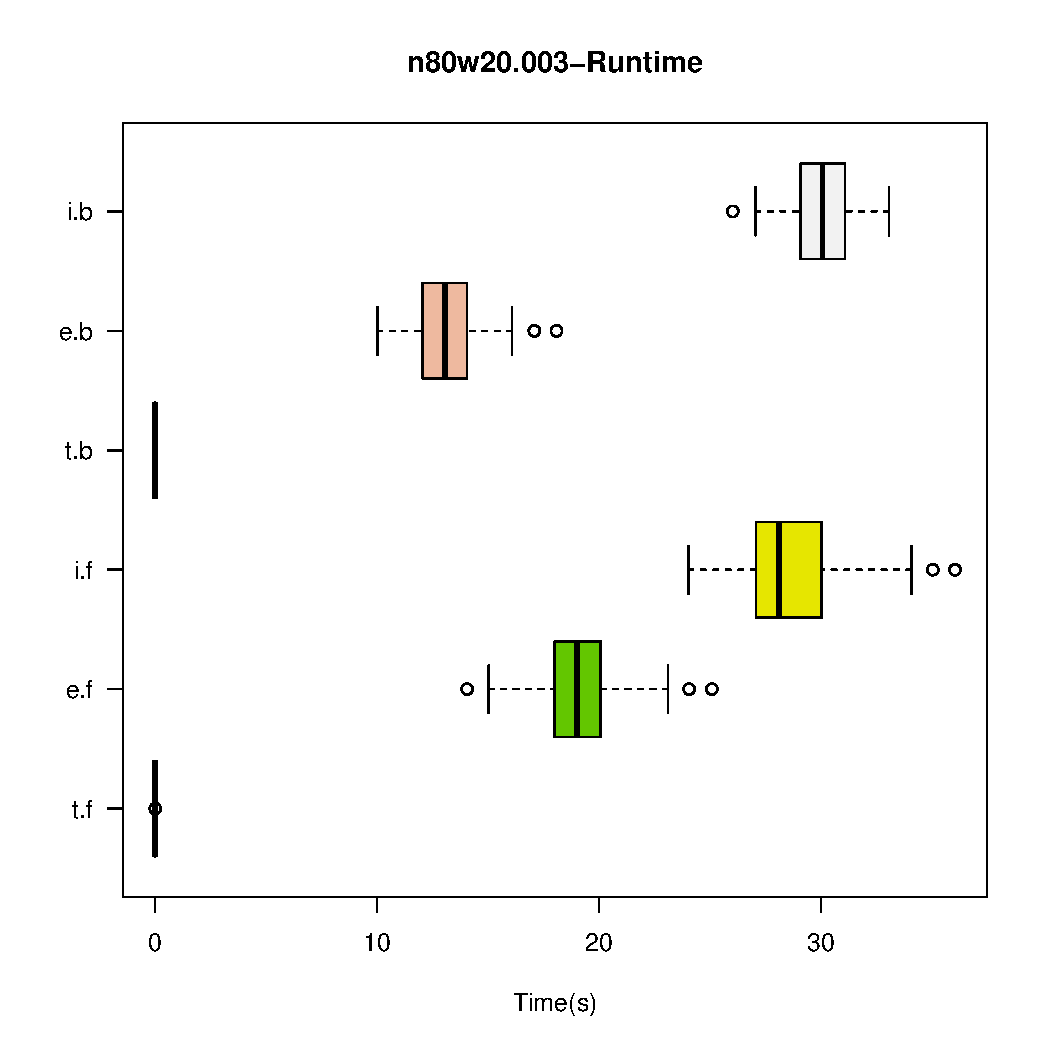
\includegraphics[width=0.6\textwidth,keepaspectratio]{{II/n80w20.003/n80w20.003-CpuTime}.pdf}
% \captionof{figure}{n80w20.003 - Runtime boxplots for the different iterative improvement algorithms}
% \end{center}

% \begin{center}
% 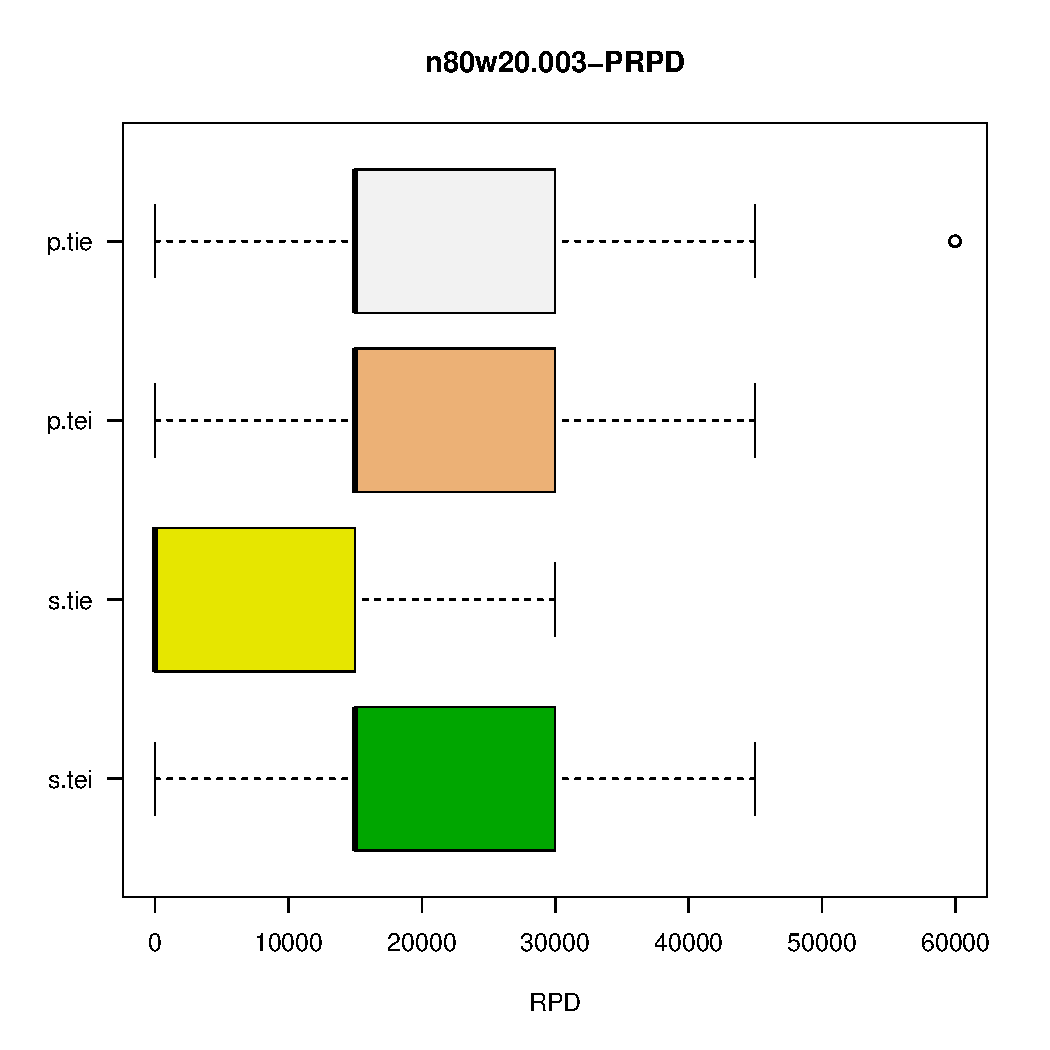
\includegraphics[width=0.6\textwidth,keepaspectratio]{{II/n80w20.003/n80w20.003-PRPD}.pdf}
% \captionof{figure}{n80w20.003 - PRPD boxplots for the different iterative improvement algorithms}
% \end{center}

% \begin{center}
% \begin{tabular}{|l|l|}
% \hline
% \textbf{Test} & \textbf{P-Value} \\
% \hline
% First vs best - Transpose&3.95591160889952e-18\\
% \hline
% First vs best - Exchange&6.21747363653032e-18\\
% \hline
% First vs best - Insert&6.2952945764779e-08\\
% \hline
% Exchange vs Insert - First&3.9556885406462e-18\\
% \hline
% Exchange vs Insert - Best&3.95591160889952e-18\\
% \hline
% \end{tabular}
% \captionof{table}{n80w20.003 - Results of Wilcoxon paired signed rank test}
% \label{tab:w.3}
% \end{center}

% \subsubsection{n80w20.004}
% \begin{center}
% 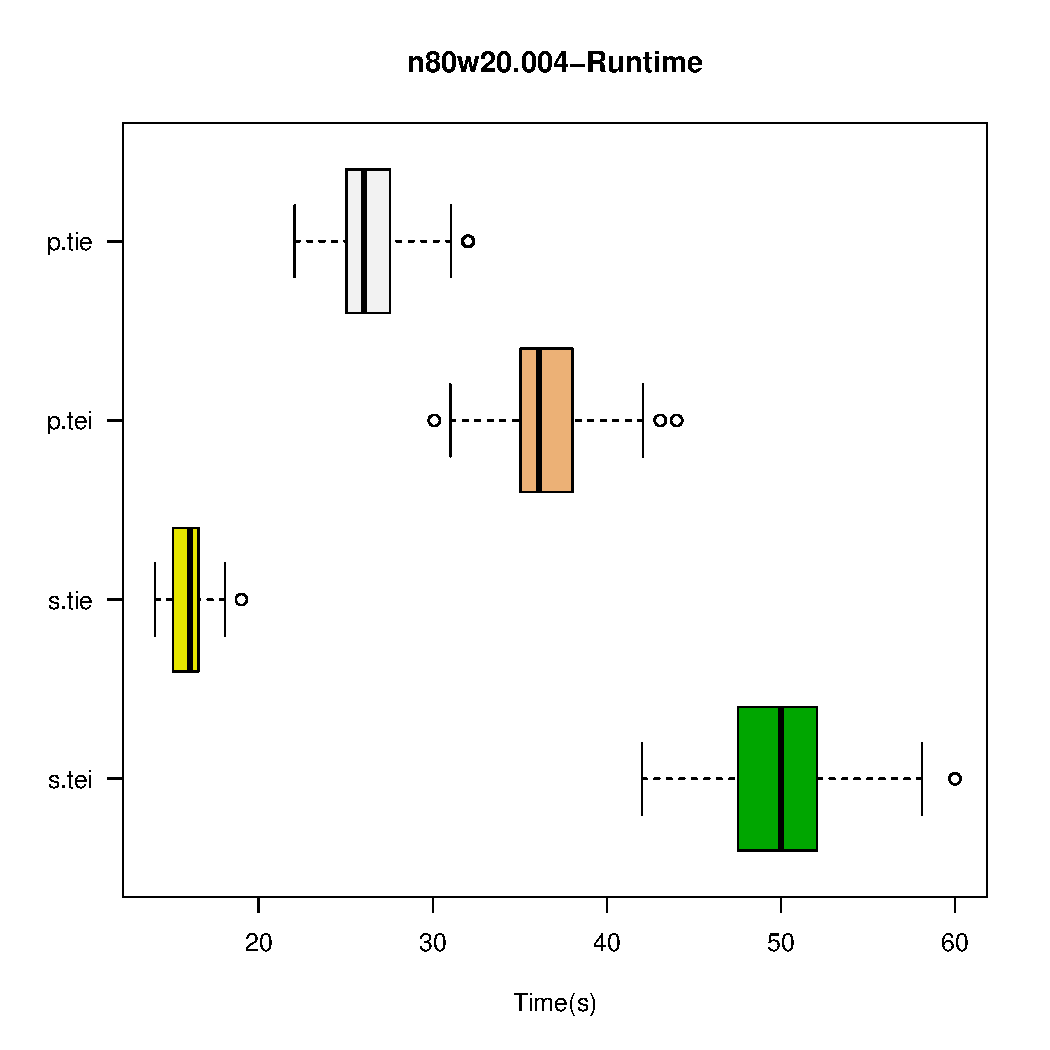
\includegraphics[width=0.6\textwidth,keepaspectratio]{{II/n80w20.004/n80w20.004-CpuTime}.pdf}
% \captionof{figure}{n80w20.004 - Runtime boxplots for the different iterative improvement algorithms}
% \end{center}

% \begin{center}
% 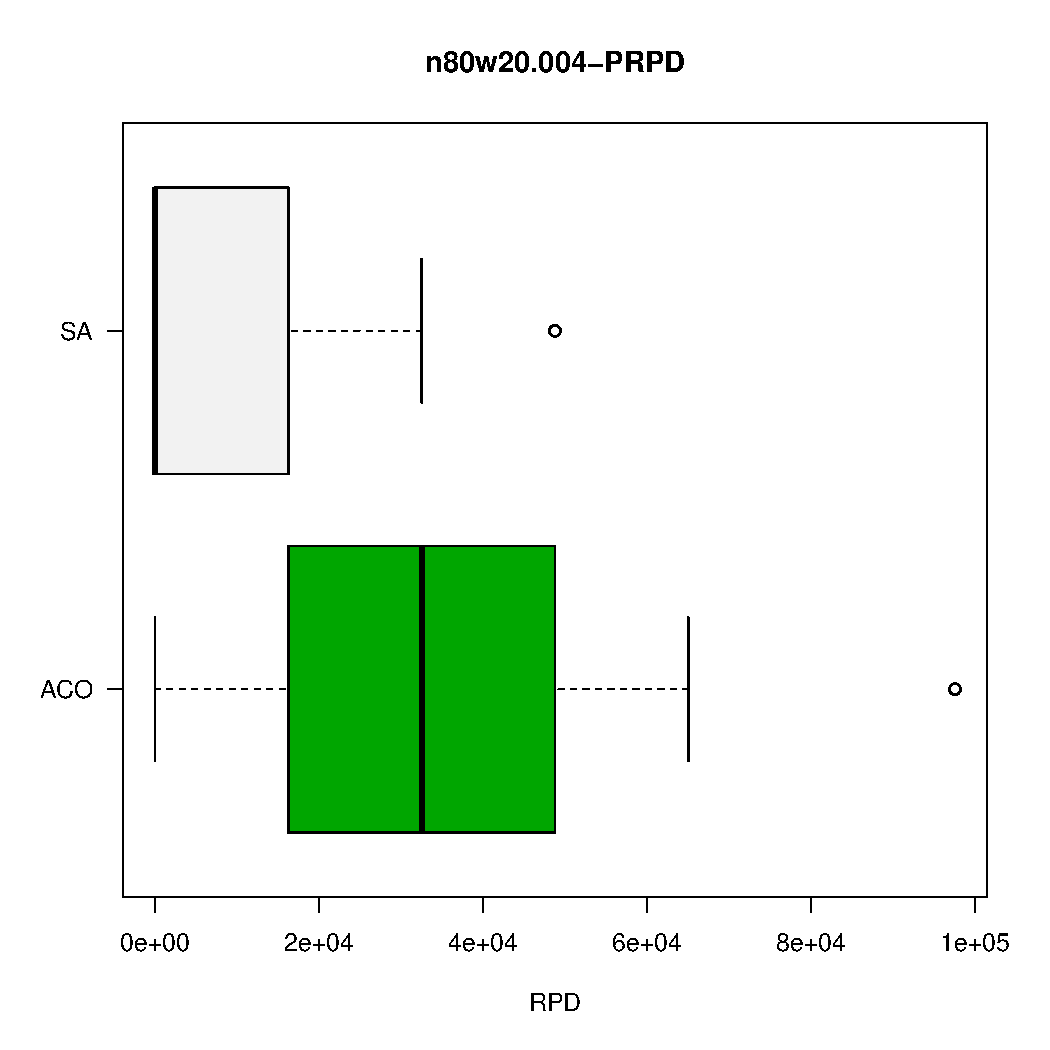
\includegraphics[width=0.6\textwidth,keepaspectratio]{{II/n80w20.004/n80w20.004-PRPD}.pdf}
% \captionof{figure}{n80w20.001 - PRPD boxplots for the different iterative improvement algorithms}
% \end{center}

% \begin{center}
% \begin{tabular}{|l|l|}
% \hline
% \textbf{Test} & \textbf{P-Value} \\
% \hline
% First vs best - Transpose&4.33123080260219e-18\\
% \hline
% First vs best - Exchange&1.5356610755813e-16\\
% \hline
% First vs best - Insert&4.27702026764362e-14\\
% \hline
% Exchange vs Insert - First&5.59593516960623e-18\\
% \hline
% Exchange vs Insert - Best&3.95591160889952e-18\\
% \hline
% \end{tabular}
% \captionof{table}{n80w20.004 - Results of Wilcoxon paired signed rank test}
% \label{tab:w.4}
% \end{center}

% \subsubsection{n80w20.005}
% \begin{center}
% 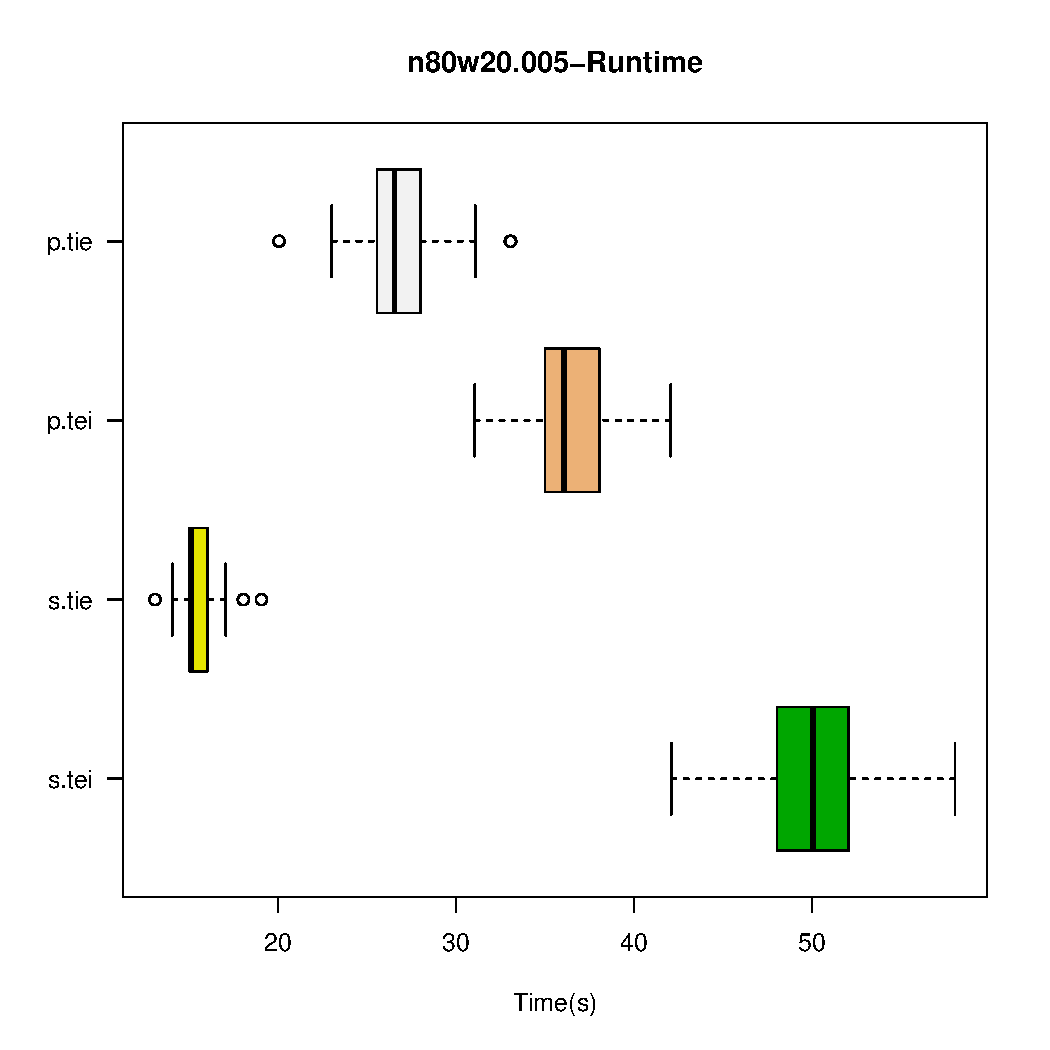
\includegraphics[width=0.6\textwidth,keepaspectratio]{{II/n80w20.005/n80w20.005-CpuTime}.pdf}
% \captionof{figure}{n80w20.005 - Runtime boxplots for the different iterative improvement algorithms}
% \end{center}

% \begin{center}
% 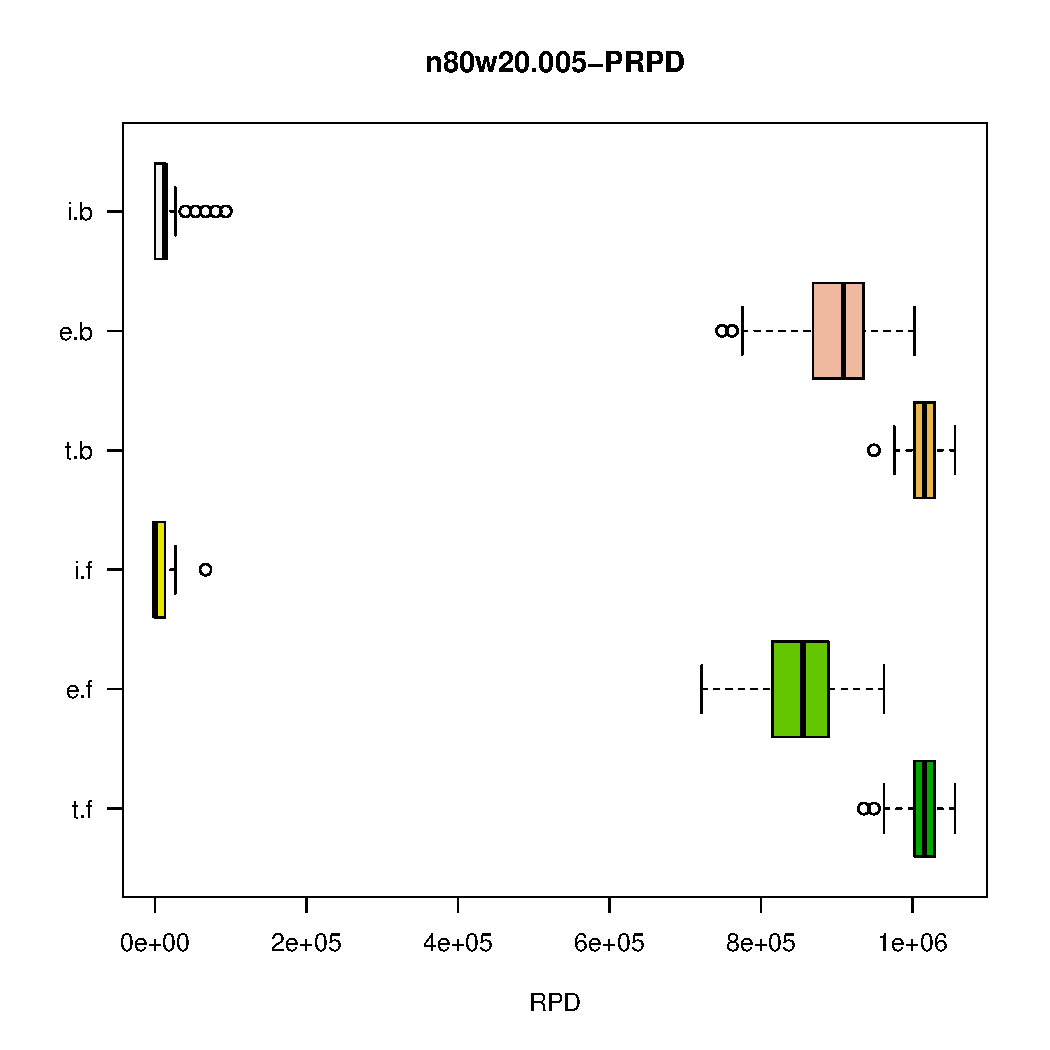
\includegraphics[width=0.6\textwidth,keepaspectratio]{{II/n80w20.005/n80w20.005-PRPD}.pdf}
% \captionof{figure}{n80w20.005 - PRPD boxplots for the different iterative improvement algorithms}
% \end{center}

% \begin{center}
% \begin{tabular}{|l|l|}
% \hline
% \textbf{Test} & \textbf{P-Value} \\
% \hline
% First vs best - Transpose&4.46398542390809e-18\\
% \hline
% First vs best - Exchange&4.74166029806301e-18\\
% \hline
% First vs best - Insert&4.0369131744045e-10\\
% \hline
% Exchange vs Insert - First&4.74166029806301e-18\\
% \hline
% Exchange vs Insert - Best&3.95591160889952e-18\\
% \hline
% \end{tabular}
% \captionof{table}{n80w20.005 - Results of Wilcoxon paired signed rank test}
% \label{tab:w.5}
% \end{center}

% \subsubsection{n80w200.001}
% \begin{center}
% \includegraphics[width=0.6\textwidth,keepaspectratio]{{II/n80w200.001/n80w200.001-CpuTime}.pdf}
% \captionof{figure}{n80w200.001 - Runtime boxplots for the different iterative improvement algorithms}
% \end{center}

% \begin{center}
% \includegraphics[width=0.6\textwidth,keepaspectratio]{{II/n80w200.001/n80w200.001-PRPD}.pdf}
% \captionof{figure}{n80w200.001 - PRPD boxplots for the different iterative improvement algorithms}
% \end{center}

% \begin{center}
% \begin{tabular}{|l|l|}
% \hline
% \textbf{Test} & \textbf{P-Value} \\
% \hline
% First vs best - Transpose&4.07730530936212e-18\\
% \hline
% First vs best - Exchange&2.17457280454137e-17\\
% \hline
% First vs best - Insert&3.95591160889952e-18\\
% \hline
% Exchange vs Insert - First&3.95591160889952e-18\\
% \hline
% Exchange vs Insert - Best&3.95591160889952e-18\\
% \hline
% \end{tabular}
% \captionof{table}{n80w200.001 - Results of Wilcoxon paired signed rank test}
% \label{tab:w.6}
% \end{center}

% \subsubsection{n80w200.002}
% \begin{center}
% \includegraphics[width=0.6\textwidth,keepaspectratio]{{II/n80w200.002/n80w200.002-CpuTime}.pdf}
% \captionof{figure}{n80w200.002 - Runtime boxplots for the different iterative improvement algorithms}
% \end{center}

% \begin{center}
% \includegraphics[width=0.6\textwidth,keepaspectratio]{{II/n80w200.002/n80w200.002-PRPD}.pdf}
% \captionof{figure}{n80w200.002 - PRPD boxplots for the different iterative improvement algorithms}
% \end{center}

% \begin{center}
% \begin{tabular}{|l|l|}
% \hline
% \textbf{Test} & \textbf{P-Value} \\
% \hline
% First vs best - Transpose&5.19043683699158e-18\\
% \hline
% First vs best - Exchange&4.6720416035814e-17\\
% \hline
% First vs best - Insert&3.95591160889952e-18\\
% \hline
% Exchange vs Insert - First&3.95591160889952e-18\\
% \hline
% Exchange vs Insert - Best&3.95591160889952e-18\\
% \hline
% \end{tabular}
% \captionof{table}{n80w200.002 - Results of Wilcoxon paired signed rank test}
% \label{tab:w.7}
% \end{center}

% \subsubsection{n80w200.003}
% \begin{center}
% \includegraphics[width=0.6\textwidth,keepaspectratio]{{II/n80w200.003/n80w200.003-CpuTime}.pdf}
% \captionof{figure}{n80w200.003 - Runtime boxplots for the different iterative improvement algorithms}
% \end{center}

% \begin{center}
% \includegraphics[width=0.6\textwidth,keepaspectratio]{{II/n80w200.003/n80w200.003-PRPD}.pdf}
% \captionof{figure}{n80w200.003 - PRPD boxplots for the different iterative improvement algorithms}
% \end{center}

% \begin{center}
% \begin{tabular}{|l|l|}
% \hline
% \textbf{Test} & \textbf{P-Value} \\
% \hline
% First vs best - Transpose&4.33123080260219e-18\\
% \hline
% First vs best - Exchange&7.01070639830382e-18\\
% \hline
% First vs best - Insert&3.95591160889952e-18\\
% \hline
% Exchange vs Insert - First&3.95591160889952e-18\\
% \hline
% Exchange vs Insert - Best&3.95591160889952e-18\\
% \hline
% \end{tabular}
% \captionof{table}{n80w200.003 - Results of Wilcoxon paired signed rank test}
% \label{tab:w.8}
% \end{center}

% \subsubsection{n80w200.004}
% \begin{center}
% 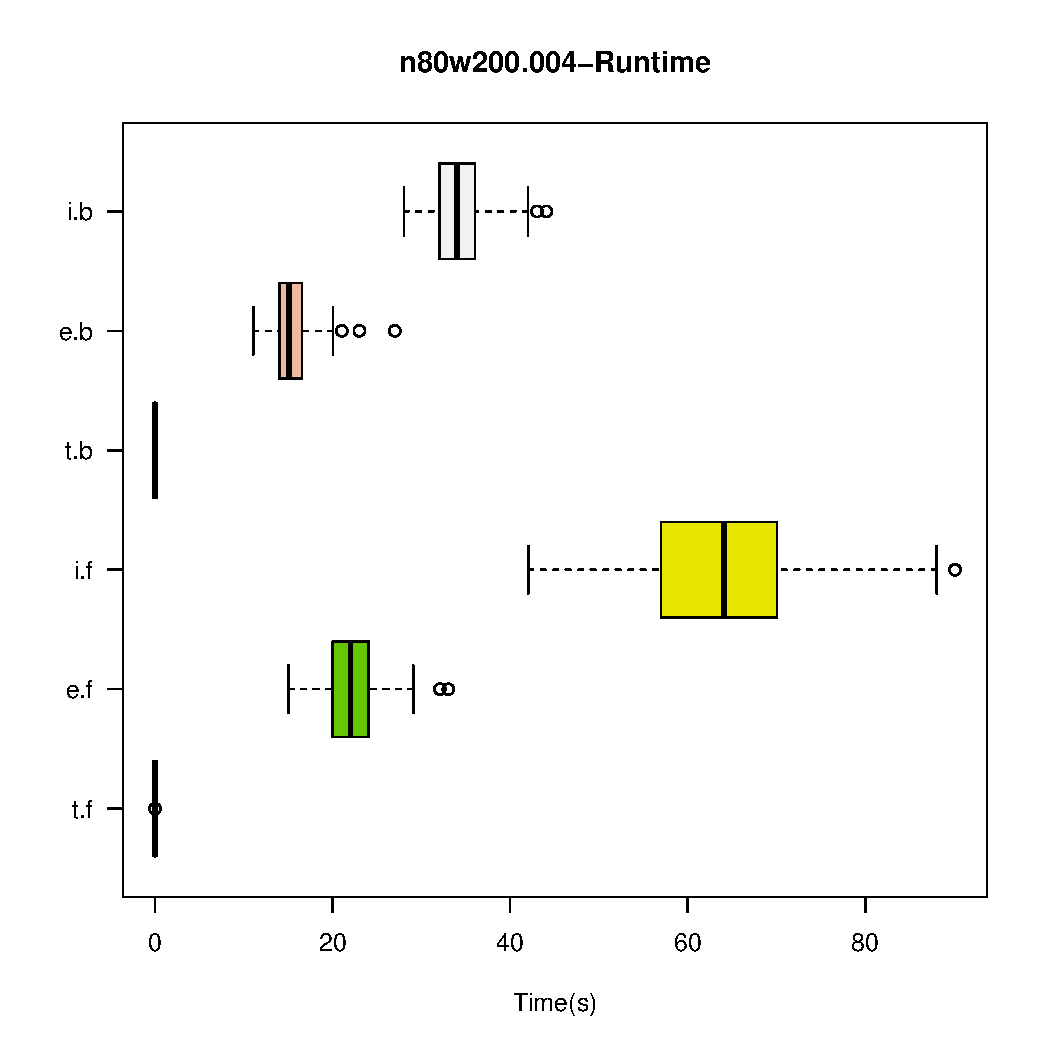
\includegraphics[width=0.6\textwidth,keepaspectratio]{{II/n80w200.004/n80w200.004-CpuTime}.pdf}
% \captionof{figure}{n80w200.004 - Runtime boxplots for the different iterative improvement algorithms}
% \end{center}

% \begin{center}
% 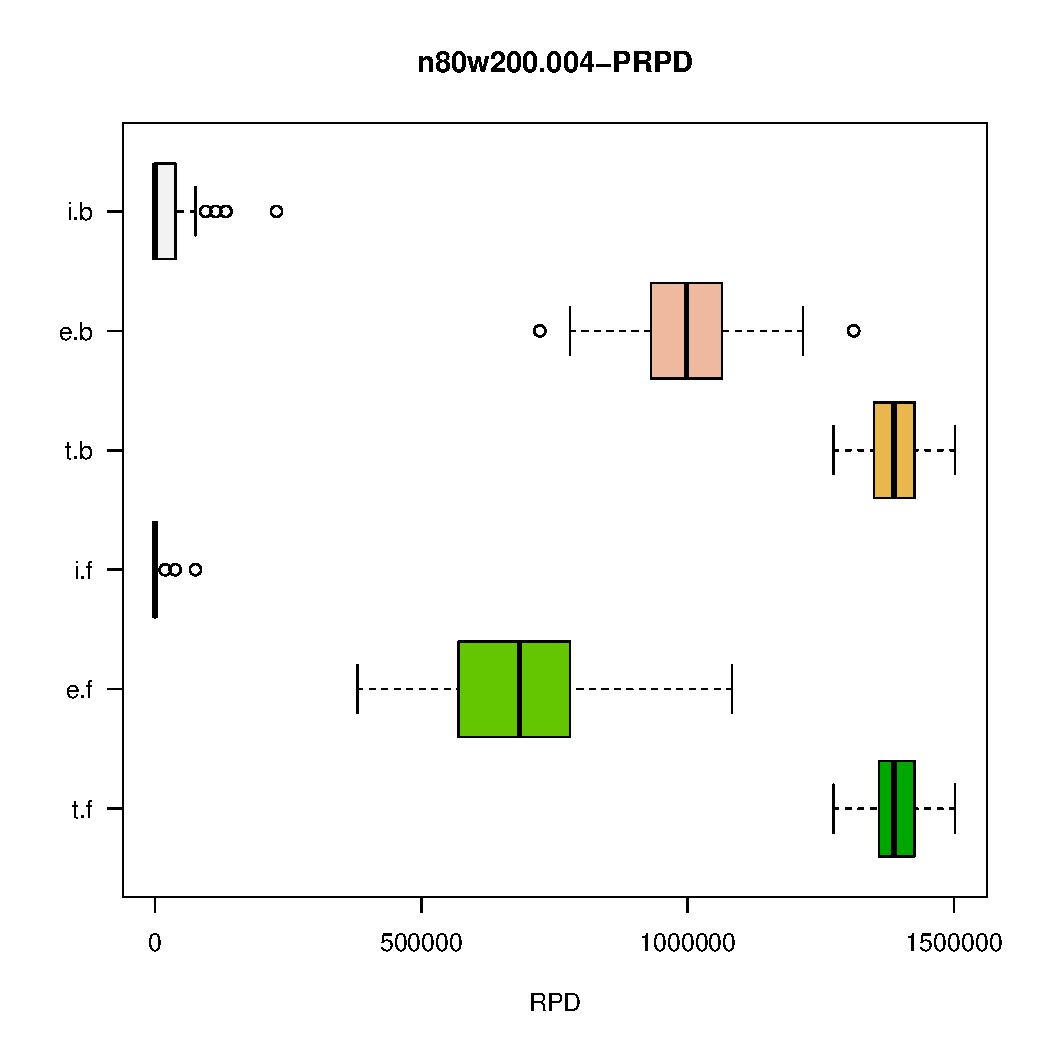
\includegraphics[width=0.6\textwidth,keepaspectratio]{{II/n80w200.004/n80w200.004-PRPD}.pdf}
% \captionof{figure}{n80w200.001 - PRPD boxplots for the different iterative improvement algorithms}
% \end{center}

% \begin{center}
% \begin{tabular}{|l|l|}
% \hline
% \textbf{Test} & \textbf{P-Value} \\
% \hline
% First vs best - Transpose&4.33123080260219e-18\\
% \hline
% First vs best - Exchange&2.4473398426105e-17\\
% \hline
% First vs best - Insert&3.95591160889952e-18\\
% \hline
% Exchange vs Insert - First&3.95591160889952e-18\\
% \hline
% Exchange vs Insert - Best&3.95591160889952e-18\\
% \hline
% \end{tabular}
% \captionof{table}{n80w200.004 - Results of Wilcoxon paired signed rank test}
% \label{tab:w.9}
% \end{center}

% \subsubsection{n80w200.005}
% \begin{center}
% 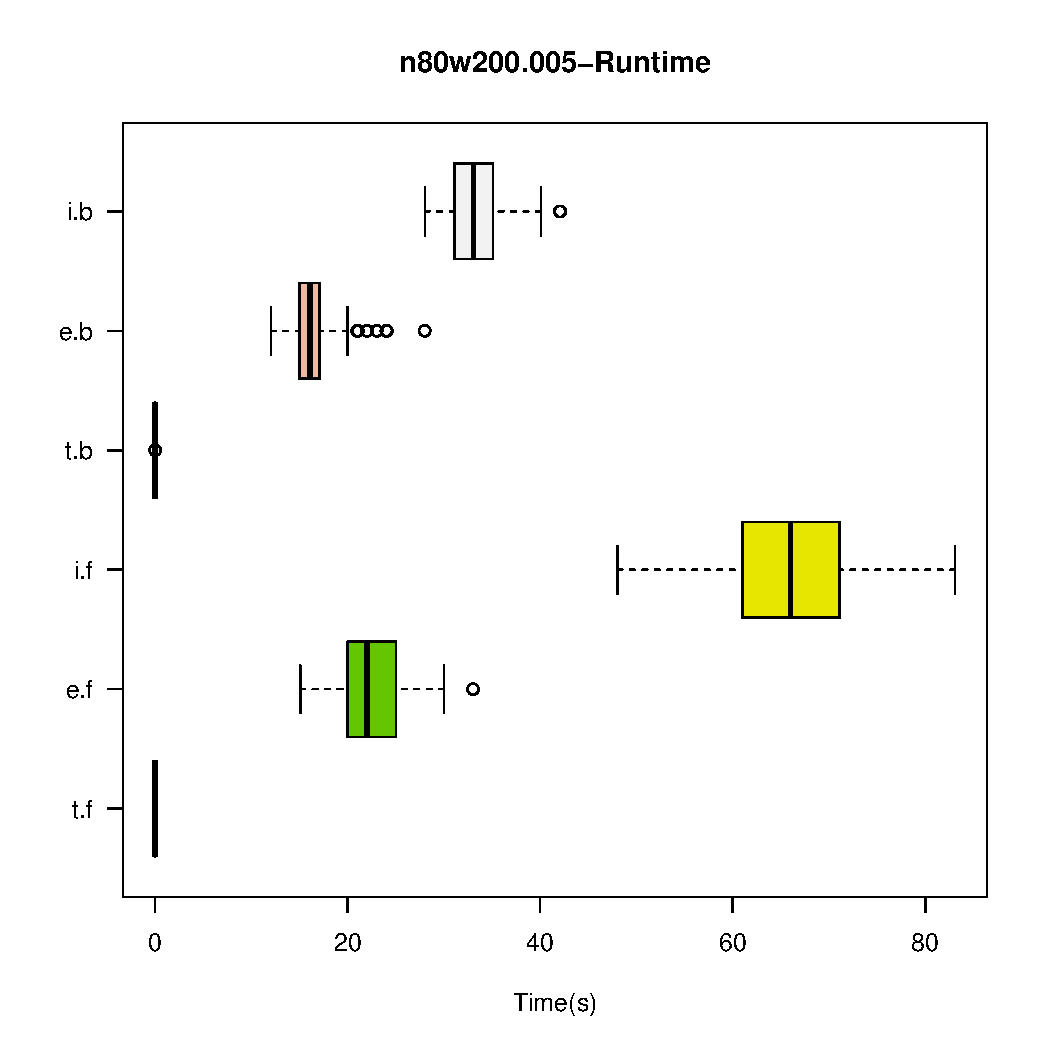
\includegraphics[width=0.6\textwidth,keepaspectratio]{{II/n80w200.005/n80w200.005-CpuTime}.pdf}
% \captionof{figure}{n80w200.005 - Runtime boxplots for the different iterative improvement algorithms}
% \end{center}

% \begin{center}
% 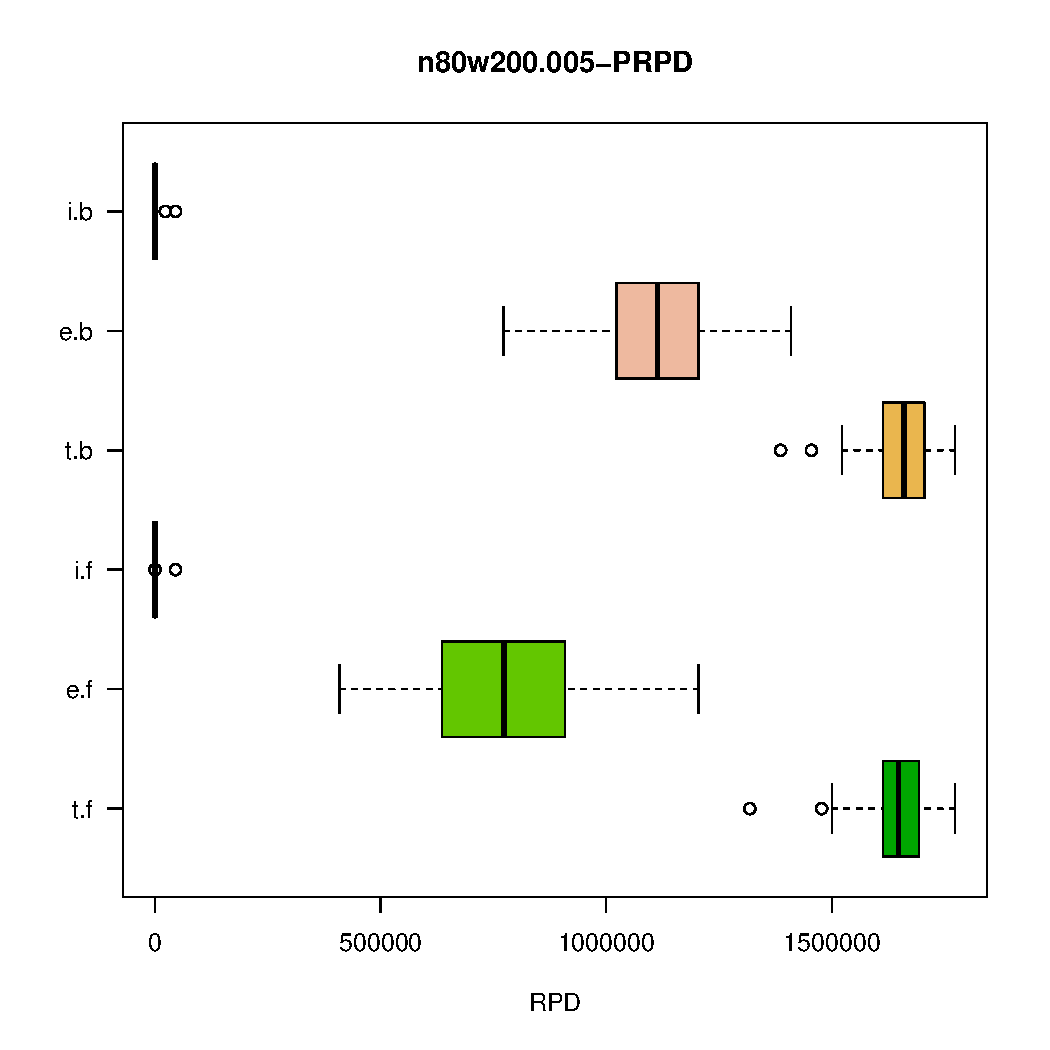
\includegraphics[width=0.6\textwidth,keepaspectratio]{{II/n80w200.005/n80w200.005-PRPD}.pdf}
% \captionof{figure}{n80w200.005 - PRPD boxplots for the different iterative improvement algorithms}
% \end{center}

% \begin{center}
% \begin{tabular}{|l|l|}
% \hline
% \textbf{Test} & \textbf{P-Value} \\
% \hline
% First vs best - Transpose&4.74166029806301e-18\\
% \hline
% First vs best - Exchange&1.40854365025687e-16\\
% \hline
% First vs best - Insert&3.95591160889952e-18\\
% \hline
% Exchange vs Insert - First&3.95591160889952e-18\\
% \hline
% Exchange vs Insert - Best&3.95591160889952e-18\\
% \hline
% \end{tabular}
% \captionof{table}{n80w200.005 - Results of Wilcoxon paired signed rank test}
% \label{tab:w.10}
% \end{center}

% \subsection{Statistics}

% \subsubsection{Transpose-First Improvement}
% \begin{center}
% \begin{tabular}{|l|c|l|l|}
% \hline
% \textbf{Instance}& \textbf{\% Infeasible} & $\mathbf{\bar{PRDP}}$ &$\mathbf{\bar{Runtime}}$\\
% \hline
% n80w20.001&1&1229712.6&0.0100035563\\
% \hline
% n80w20.002&1&1028075.17&0.0095843375\\
% \hline
% n80w20.003&1&1132968.5&0.0098099452\\
% \hline
% n80w20.005&1&1010681.79&0.0097989762\\
% \hline
% n80w20.004&1&1226174.6&0.0094877067\\
% \hline
% n80w200.001&1&1467634.1&0.0098152878\\
% \hline
% n80w200.002&1&1504523.7&0.0099101404\\
% \hline
% n80w200.004&1&1388037.6&0.0098893615\\
% \hline
% n80w200.003&1&1567210.5&0.0097697727\\
% \hline
% n80w200.005&1&1644110.9&0.0097550971\\
% \hline
% \end{tabular}
% \captionof{table}{Statistics summary for iterative improvement algorithm with Transpose neighborhood and First Improvement pivoting rule}
% \label{tab:t.f}
% \end{center}

% \subsubsection{Transpose-Best Improvement}
% \begin{center}
% \begin{tabular}{|l|c|l|l|}
% \hline
% \textbf{Instance}& \textbf{\% Infeasible} & $\mathbf{\bar{PRDP}}$ &$\mathbf{\bar{Runtime}}$\\
% \hline
% n80w20.001&1&1236039.3&0.014545497\\
% \hline
% n80w20.002&1&1033090.48&0.0145450422\\
% \hline
% n80w20.003&1&1137758.7&0.014536776\\
% \hline
% n80w20.005&1&1014818.46&0.014947609\\
% \hline
% n80w20.004&1&1232996&0.015151286\\
% \hline
% n80w200.001&1&1476994.8&0.0147534638\\
% \hline
% n80w200.002&1&1511281&0.014884921\\
% \hline
% n80w200.004&1&1392023.3&0.0146445173\\
% \hline
% n80w200.003&1&1575355.5&0.0143582468\\
% \hline
% n80w200.005&1&1653419.6&0.0150098656\\
% \hline
% \end{tabular}
% \captionof{table}{Statistics summary for iterative improvement algorithm with Transpose neighborhood and Best Improvement pivoting rule}
% \label{tab:t.b}
% \end{center}

% \subsubsection{Exchange-First Improvement}
% \begin{center}
% \begin{tabular}{|l|c|l|l|}
% \hline
% \textbf{Instance}& \textbf{\% Infeasible} & $\mathbf{\bar{PRDP}}$ &$\mathbf{\bar{Runtime}}$\\
% \hline
% n80w20.001&1&1035718.78&18.390814\\
% \hline
% n80w20.002&1&884386.3&18.198632\\
% \hline
% n80w20.003&1&956518.77&18.913801\\
% \hline
% n80w20.005&1&849054.52&19.043496\\
% \hline
% n80w20.004&1&1030411.56&19.660314\\
% \hline
% n80w200.001&1&661322.18&23.117446\\
% \hline
% n80w200.002&1&813339.6&22.552976\\
% \hline
% n80w200.004&1&679489.06&22.068859\\
% \hline
% n80w200.003&1&697450.03&24.338257\\
% \hline
% n80w200.005&1&760027.65&22.348975\\
% \hline
% \end{tabular}
% \captionof{table}{Statistics summary for iterative improvement algorithm with Exchange neighborhood and First Improvement pivoting rule}
% \label{tab:e.f}
% \end{center}

% \subsubsection{Exchange-Best Improvement}
% \begin{center}
% \begin{tabular}{|l|c|l|l|}
% \hline
% \textbf{Instance}& \textbf{\% Infeasible} & $\mathbf{\bar{PRDP}}$ &$\mathbf{\bar{Runtime}}$\\
% \hline
% n80w20.001&1&1086217.68&13.091453\\
% \hline
% n80w20.002&1&901762.05&13.365301\\
% \hline
% n80w20.003&1&1017243.86&13.267128\\
% \hline
% n80w20.005&1&895720.53&13.5824245\\
% \hline
% n80w20.004&1&1084080.4&14.189582\\
% \hline
% n80w200.001&1&1022433.76&16.418229\\
% \hline
% n80w200.002&1&1075649.94&16.028712\\
% \hline
% n80w200.004&1&994703.67&15.518766\\
% \hline
% n80w200.003&1&1094460.9&16.16696\\
% \hline
% n80w200.005&1&1110949.86&16.566802\\
% \hline
% \end{tabular}
% \captionof{table}{Statistics summary for iterative improvement algorithm with Exchange neighborhood and Best Improvement pivoting rule}
% \label{tab:e.b}
% \end{center}

% \subsubsection{Insert-First Improvement}
% \begin{center}
% \begin{tabular}{|l|c|l|l|}
% \hline
% \textbf{Instance}& \textbf{\% Infeasible} & $\mathbf{\bar{PRDP}}$ &$\mathbf{\bar{Runtime}}$\\
% \hline
% n80w20.001&0.65&16070.27322082&25.88279\\
% \hline
% n80w20.002&0.83&11803.71462682&28.509938\\
% \hline
% n80w20.003&0.83&21587.617&28.579453\\
% \hline
% n80w20.005&0.32&4945.642107&28.672083\\
% \hline
% n80w20.004&0.49&10894.01867489&28.474429\\
% \hline
% n80w200.001&0.22&6119.9927045&59.544212\\
% \hline
% n80w200.002&0&11.2561521&64.580306\\
% \hline
% n80w200.004&0.11&3049.80805246&63.942238\\
% \hline
% n80w200.003&0.01&437.87774695&63.687806\\
% \hline
% n80w200.005&0.01&464.62990671&66.084369\\
% \hline
% \end{tabular}
% \captionof{table}{Statistics summary for iterative improvement algorithm with Insert neighborhood and First Improvement pivoting rule}
% \label{tab:i.f}
% \end{center}

% \subsubsection{Insert-Best Improvement}
% \begin{center}
% \begin{tabular}{|l|c|l|l|}
% \hline
% \textbf{Instance}& \textbf{\% Infeasible} & $\mathbf{\bar{PRDP}}$ &$\mathbf{\bar{Runtime}}$\\
% \hline
% n80w20.001&0.56&14772.44442862&28.769951\\
% \hline
% n80w20.002&0.84&16009.51797952&30.159812\\
% \hline
% n80w20.003&0.89&26984.256&30.197019\\
% \hline
% n80w20.005&0.52&10159.3062354&30.776906\\
% \hline
% n80w20.004&0.59&18861.32619536&31.013\\
% \hline
% n80w200.001&0.37&21195.2243605&33.031965\\
% \hline
% n80w200.002&0&13.2172159&33.011011\\
% \hline
% n80w200.004&0.42&23019.4946845&34.123681\\
% \hline
% n80w200.003&0.12&7740.06242146&34.080592\\
% \hline
% n80w200.005&0.07&2516.0079072&33.450537\\
% \hline
% \end{tabular}
% \captionof{table}{Statistics summary for iterative improvement algorithm with Insert neighborhood and Best Improvement pivoting rule}
% \label{tab:i.b}
% \end{center}

% \subsection{Results discussion}
% By looking at tables \ref{tab:t.f}, \ref{tab:t.b}, \ref{tab:e.f}, \ref{tab:e.b} \ref{tab:i.f}, \ref{tab:i.b} on can see that:
% \begin{itemize}
% \item The neighborhood type has a strong influence on the both the time complexity of the algorithm and the generated solution quality. This is due to the size of the different neighborhoods ($n=80$):
%       \begin{itemize}
%         \item Transpose - $(n-1)$
%         \item Exchange - $\frac{n\cdot(n-1)}{2}$
%         \item Insert - $(n-1)^2$
%       \end{itemize}
% The different size of the neighborhoods corresponds to different degrees of exploration (diversification).
      
% \item Transpose and Exchange neighborhoods have smaller runtimes but a percentage of infeasible runs equal to 1. 
% Both the algorithm do not allow to find a feasible solution but the Exchange algorithm constructs solutions with a better quality (reduced, but not yet null, constraint violations and total travel time).

% \item Insert is the only neighborhood type that allows to generate solutions that are both feasible and closer to the global optima.

% \item The first-improvement pivoting rule is generally slower than the best-improvement one, when considering the same neighborhood type.
% This is due to the fact that, with the first-improvement pivoting rule, smaller improvement are made to the solution at each iteration, thus requiring and higher number of iteration to converge to a local optima, with respect to the case where the best improvement is chosen at each time step.

% \item The quality of the solutions generated using the first-improvement pivoting rule is slightly better thant those generated using the best-improvement one.

% \item Tables \ref{tab:w.1}, \ref{tab:w.2}, \ref{tab:w.3}, \ref{tab:w.4}, \ref{tab:w.5}, \ref{tab:w.6}, \ref{tab:w.7}, \ref{tab:w.8}, \ref{tab:w.9}, \ref{tab:w.10} contain, in any case, p-values considerably smaller than the significance level ($\alpha=0.05$). 

% This implies that the null hypothesis corresponding to the equality of the median values of the differences of the two distributions can be rejected, hence assessing the existence of a statistically significant difference among the solution quality generated by analyzed algorithms.

% \item By looking at the Cpu time, one can easily see that the instances \emph{n80w20.X} have lower runtimes than the \emph{n80w200.X} ones. They can then be considered, with respect to the iterative improvement algorithms, simpler instances with respect to the latter.

% \end{itemize}

\end{homeworkProblem}		

\section{Results} \label{results}
\subsection{Metric definitions}\label{subsec:metric}
For each algorithm $A$, applied on instance $i$, using different randomly generated seeds one have to compute:
\begin{itemize}
  \item  Percentage of runs with constraint violations (0.xxyyy has to be interpreted as xx.yyy\%)
  \item  Mean penalized relative percentage deviation
\end{itemize}

In order to compute these statistics, each algorithm $A$ is launched 25 times on the same instance, measuring the following quantities on each run:
\begin{itemize}
  \item Constraint violations at the end of the run  
  \item Penalized relative percentage deviation of the final solution with respect to the optimal one.
  \item Computation time (CPU time).
\end{itemize}

For each instance $i$, the distributions of PRPD are also displayed using box-plots and tested using the Wilcoxon signed rank statistical test, in order to assess the existence of a statistically significant difference among the results obtained by the different algorithms (ACO and SA) on the same instance. 

\paragraph{Constraint Violations}
In the standard formulation of the TSP problem, a solution to the problem is represented by a permutation of the different
entities (solution components), that the hypothetical traveling salesman has to visit.

The best solution for the problem is the permutation that minimizes the total traveling time (distance) among the cities.
The presence of time windows introduce an additional constraint on the feasibility of the solution.

In fact, each solution component has an associated time window within which it has to be visited in order to guarantee the feasibility of the tour.

Arriving in a (city) before the opening of the corresponding time window involves a delay in the total traveling time (to wait for the time window to open) whereas the arrival after the closure of the time windows will generate a constraint violation.

Thus, a solution is feasible if and only if all the time windows constraints are met, or in other words, if there are no constraint violations.

In this case, the best solution is the feasible solution which minimizes the total travel time.

\paragraph{Penalized Relative Percentage Deviation}
The penalized relative percentage deviation (PRDP from now on) is a measure of the solution quality, with respect to the best known solution for the instance, taking into account a strong penalization for the violation of constraints.

The PRPD is computed as follows:
\begin{equation}
pRPD_{kri} = 100 \cdot \frac{(f_{kri} + 10^4\cdot\Omega_{kri})-best_i}{best_i}
\end{equation}

\paragraph{Run-time}
The run-time is a measure of both the quality and the time complexity of the algorithm.

It is measured using the function \verb|int clock_gettime(clockid_t clk_id, struct timespect *tp)| from the \verb|time.h| library.

The parameter \verb|clk_id=CLOCK_PROCESS_CPUTIME_ID|, is used to read the values from an high-resolution timer provided by the CPU for each process.

The run-time is computed (using the user defined function \verb|ComputeRunTime|) as the difference, with a resolution of $10^-9$ s, from the time obtained using \verb|clock_gettime| at the beginning and the one obtained at the end of the simulation.


\subsection{Run-time distribution}
\subsubsection{Formal definition}
Given an SLS algorithm $A$ and an optimization problem $\Pi$, the success probability of $A$ on a given instance $\pi \in \Pi$ is defined as: 
\begin{equation}
  P_s[RT_{A,\pi} \le t,SQ_{A,\pi} \le q]
\end{equation}

That is, the probability of finding a solution of the problem whose quality is less or equal than $q$ in a time smaller or equal than $t$.

The solution quality $q$ is often expressed as relative solution quality:
\begin{equation}
  q_r = \frac{q}{q_b} - 1
\end{equation}

where $q_b$ is the solution quality of the best known solution for the considered instance $\pi$.

The run-time distribution of $A$ on $\pi$ consists of the probability distribution of the bi-variate random variable ($RT_{A,\pi},SQ_{A,\pi}$).

In other words, the run-time distribution can be defined as: 
\begin{equation}
  RTD_{A,\pi}(t,q) = P_s[RT_{a,\pi} \le t,SQ_{a,\pi} \le q]
\end{equation}

$RTD:\mathbb{R}^{+} \times \mathbb{R}^{+} \mapsto [0,1]$ is indeed a function, defined for algorithm $A$ on instance $\pi \in \Pi$, that maps to each pair run-time $t$, solution quality $q$ the corresponding success probability.


On one hand, by fixing the solution quality to a certain value $q^{*}$ one can obtain the qualified run-time distribution:
\begin{equation}
  QRTD_{A,\pi,q^{*}}(t) = RTD_{A,\pi}(t,q^{*}) = P_s[RT_{a,\pi} \le t,SQ_{a,\pi} \le q^{*}]
\end{equation}

which represents the probability of finding a solution of a better quality than $q^{*}$ as a function of the run-time $t$.


On the other hand, by fixing the maximum computation time to the value $t^{*}$ one obtains the solution quality distribution:
\begin{equation}
  SQD_{A,\pi,t^{*}}(q) = RTD_{A,\pi}(t^{*},q) = P_s[RT_{a,\pi} \le t^{*},SQ_{a,\pi} \le q]
\end{equation}

which determines the probability of finding a solution having a certain quality $q$ given the time bound $t^{*}$.

These are marginal distributions of the run-time one, which allow to have a better insight, respectively, on the time required for the algorithm to find a reasonably good solution and conversely, on the solution quality that can be obtained by fixing a computation time bound, of the algorithm $A$ on instance $\pi$.

\subsubsection{Measurement}\label{subsec:measure}
In the case of the Travel ling Salesman Problem with Time Windows, the algorithm has not only to minimize the total Travel ling time, but also respect all the constraints determined by the time window of each of the nodes.

The solution quality is defined by aggregating the two objectives and taking into account a penalization $p_e = 10^4$ for each constraint violations:
\begin{equation}
  q(p) = f(p) + p_e \cdot\Omega(p)
\end{equation}

from which
\begin{equation}
  q_r(p) = \frac{q(p)}{q_{best}} - 1
\end{equation}

It should be noted that, since the number of constraint violations $\Omega(p)$ constitutes a hard constraint on the feasibility of the solution, the value of the penality $p_e$ is at least ten times bigger than the magnitude of the worst solutions.

This implies that infeasible solutions with a shorter tour with respect to the optimal one, will have an higher relative solution quality $q_r$ than worse but yet feasible solutions.

The measurement of the run-time distributions to reach sufficiently high quality solution, of the implemented algorithms, consists indeed in the estimation of the qualified run-time distribution $QRTD_{A,\pi,q_r^{*}}(t)$ for a sufficiently high relative solution quality $q_r^{*} \in (0,0.025)$.

By running the algorithms for a reasonable number of repetitions the success probability $P_s$ can be approximated by the relative observed frequencies as:
\begin{equation}
P_s[RT_{A,\pi} \le t,RSQ_{A,\pi} \le q_r^{*}] \approx \frac{\text{\#repetitions s.t. } (RT_{A,\pi} \le t \wedge RSQ_{A,\pi} \le q_r^{*})}{\text{\#repetitions}}   
\end{equation}

To compute the relative frequencies, the solution quality will be measured at regular intervals of time in order to have enough samples to ensure a good quality plot.
Since the time scale of the plot will be logarithmic, the sampling process will occur in a way that every interval $[10^i,10^{i+1}]$ will contain the same number $s=50$ of relative solution qualites samples.

\subsection{Results} 

% Measure, for each of the implemented algorithms on 5 instances, the run-time distributions to reach suf-
% ficiently high quality solutions (e.g. best-known solutions available at http://iridia.ulb.ac.be/
%  ̃manuel/tsptw-instances#instances).
% Measure the run-time distributions across 25 repetitions using a cut-off time of 10 times the termination
% criterion above.

% In addition to the randomly generated initial function, I developed the \verb|GenerateHeuristicInitialSolution()|
% which construct the initial solution according to an heuristic which aims to minimize the number of constraint violations.

% The general outline of the algorithm is as follows:
% \begin{enumerate}
%   \item Construct a solution by ordering the solution components in an ascending way according to their time windows closing time
%   \item For a number of times equal to the solution size divided by 10:
%   \begin{enumerate}
%     \item Select a random solution component in the solution
%     \item Select a neighborhood size randomly.
%     \item Shuffle the elements in the chosen neighborhood of the chosen solution
%   \end{enumerate}
% \end{enumerate}

% Due to the lack of time, I was only able to test the heuristic function on a limited number of instances.
% The same metrics as in \ref{subsec:metric} will be used to evaluate the algorithms.

% \subsubsection{n80w200.001}
% \begin{center}
% \includegraphics[width=0.6\textwidth,keepaspectratio]{{II-H/n80w200.001-CpuTime}.pdf}
% \captionof{figure}{n80w200.001 - Runtime boxplots for the different iterative improvement algorithms with heuristic initialization}
% \end{center}

% \begin{center}
% \includegraphics[width=0.6\textwidth,keepaspectratio]{{II-H/n80w200.001-PRPD}.pdf}
% \captionof{figure}{n80w200.001 - PRPD boxplots for the different iterative improvement algorithms with heuristic initialization}
% \end{center}

% \begin{center}
% \begin{tabular}{|l|l|}
% \hline
% \textbf{Test} & \textbf{P-Value} \\
% \hline
% First vs best - Transpose&3.95591160889952e-18\\
% \hline
% First vs best - Exchange&3.95591160889952e-18\\
% \hline
% First vs best - Insert&7.16468868599392e-06\\
% \hline
% Exchange vs Insert - First&3.95591160889952e-18\\
% \hline
% Exchange vs Insert - Best&3.9550194074242e-18\\
% \hline
% \end{tabular}
% \captionof{table}{n80w200.001 - Results of Wilcoxon paired signed rank test}
% \label{tab:w.21}
% \end{center}

% \subsubsection{n80w200.002}
% \begin{center}
% \includegraphics[width=0.6\textwidth,keepaspectratio]{{II-H/n80w200.002-CpuTime}.pdf}
% \captionof{figure}{n80w200.002 - Runtime boxplots for the different iterative improvement algorithms with heuristic initialization}
% \end{center}

% \begin{center}
% \includegraphics[width=0.6\textwidth,keepaspectratio]{{II-H/n80w200.002-PRPD}.pdf}
% \captionof{figure}{n80w200.002 - PRPD boxplots for the different  iterative improvement algorithms with heuristic initialization}
% \end{center}

% \begin{center}
% \begin{tabular}{|l|l|}
% \hline
% \textbf{Test} & \textbf{P-Value} \\
% \hline
% First vs best - Transpose&3.95591160889952e-18\\
% \hline
% First vs best - Exchange&3.95591160889952e-18\\
% \hline
% First vs best - Insert&1.5011633635878e-17\\
% \hline
% Exchange vs Insert - First&3.95591160889952e-18\\
% \hline
% Exchange vs Insert - Best&3.9552424399092e-18\\
% \hline
% \end{tabular}
% \captionof{table}{n80w200.002 - Results of Wilcoxon paired signed rank test}
% \label{tab:w.22}
% \end{center}

% \subsubsection{n80w200.003}
% \begin{center}
% \includegraphics[width=0.6\textwidth,keepaspectratio]{{II-H/n80w200.003-CpuTime}.pdf}
% \captionof{figure}{n80w200.003 - Runtime boxplots for the different iterative improvement algorithms with heuristic initialization}
% \end{center}

% \begin{center}
% \includegraphics[width=0.6\textwidth,keepaspectratio]{{II-H/n80w200.003-PRPD}.pdf}
% \captionof{figure}{n80w200.003 - PRPD boxplots for the different iterative improvement algorithms with heuristic initialization}
% \end{center}

% \begin{center}
% \begin{tabular}{|l|l|}
% \hline
% \textbf{Test} & \textbf{P-Value} \\
% \hline
% First vs best - Transpose&3.95591160889952e-18\\
% \hline
% First vs best - Exchange&3.95591160889952e-18\\
% \hline
% First vs best - Insert&2.88431649979563e-16\\
% \hline
% Exchange vs Insert - First&3.9556885406462e-18\\
% \hline
% Exchange vs Insert - Best&4.33074349739998e-18\\
% \hline
% \end{tabular}
% \captionof{table}{n80w200.003 - Results of Wilcoxon paired signed rank test}
% \label{tab:w.23}
% \end{center}

% \subsection{Statistics}

% \subsubsection{Transpose-First Improvement}
% \begin{center}
% \begin{tabular}{|l|c|l|l|}
% \hline
% \textbf{Instance}& \textbf{\% Infeasible} & $\mathbf{\bar{PRDP}}$ &$\mathbf{\bar{Runtime}}$\\
% \hline
% n80w200.003&1&1268365.4&0.0065871265\\
% \hline
% n80w200.002&1&1071407.7&0.007598828\\
% \hline
% n80w200.001&1&1243295.2&0.0093113496\\
% \hline
% \end{tabular}
% \captionof{table}{Statistics summary for iterative improvement algorithm with Transpose neighborhood and First Improvement pivoting rule}
% \label{tab:t.f.h}
% \end{center}

% \subsubsection{Transpose-Best Improvement}
% \begin{center}
% \begin{tabular}{|l|c|l|l|}
% \hline
% \textbf{Instance}& \textbf{\% Infeasible} & $\mathbf{\bar{PRDP}}$ &$\mathbf{\bar{Runtime}}$\\
% \hline
% n80w200.003&1&1266853.5&0.0106505552\\
% \hline
% n80w200.002&1&1071417.8&0.011013054\\
% \hline
% n80w200.001&1&1240638.1&0.013889943\\
% \hline
% \end{tabular}
% \captionof{table}{Statistics summary for iterative improvement algorithm with Transpose neighborhood and Best Improvement pivoting rule}
% \label{tab:t.b.h}
% \end{center}

% \subsubsection{Exchange-First Improvement}
% \begin{center}
% \begin{tabular}{|l|c|l|l|}
% \hline
% \textbf{Instance}& \textbf{\% Infeasible} & $\mathbf{\bar{PRDP}}$ &$\mathbf{\bar{Runtime}}$\\
% \hline
% n80w200.003&0&27.068636&6.0144574\\
% \hline
% n80w200.002&0.02&432.979367&6.1109123\\
% \hline
% n80w200.001&0.87&18146.162472&8.842327\\
% \hline
% \end{tabular}
% \captionof{table}{Statistics summary for iterative improvement algorithm with Exchange neighborhood and First Improvement pivoting rule}
% \label{tab:e.f.h}
% \end{center}

% \subsubsection{Exchange-Best Improvement}
% \begin{center}
% \begin{tabular}{|l|c|l|l|}
% \hline
% \textbf{Instance}& \textbf{\% Infeasible} & $\mathbf{\bar{PRDP}}$ &$\mathbf{\bar{Runtime}}$\\
% \hline
% n80w200.003&1&180715.273&17.098637\\
% \hline
% n80w200.002&1&92647.622&12.3893899\\
% \hline
% n80w200.001&1&694332.77&17.575257\\
% \hline
% \end{tabular}
% \captionof{table}{Statistics summary for iterative improvement algorithm with Exchange neighborhood and Best Improvement pivoting rule}
% \label{tab:e.b.h}
% \end{center}

% \subsubsection{Insert-First Improvement}
% \begin{center}
% \begin{tabular}{|l|c|l|l|}
% \hline
% \textbf{Instance}& \textbf{\% Infeasible} & $\mathbf{\bar{PRDP}}$ &$\mathbf{\bar{Runtime}}$\\
% \hline
% n80w200.003&0.03&2587.6121429&30.841123\\
% \hline
% n80w200.002&0&9.9979528&35.672697\\
% \hline
% n80w200.001&0.1&4897.5213208&32.775532\\
% \hline
% \end{tabular}
% \captionof{table}{Statistics summary for iterative improvement algorithm with Insert neighborhood and First Improvement pivoting rule}
% \label{tab:i.f.h}
% \end{center}

% \subsubsection{Insert-Best Improvement}
% \begin{center}
% \begin{tabular}{|l|c|l|l|}
% \hline
% n80w200.003&0&4.3454898&23.452399\\
% \hline
% n80w200.002&0.01&630.9635938&27.922795\\
% \hline
% n80w200.001&0.1&3680.5235577&32.277408\\
% \hline
% \end{tabular}
% \captionof{table}{Statistics summary for iterative improvement algorithm with Insert neighborhood and Best Improvement pivoting rule}
% \label{tab:i.b.h}
% \end{center}

% \subsection{Results discussion}
% By looking at tables \ref{tab:t.f.h}, \ref{tab:t.b.h}, \ref{tab:e.f.h}, \ref{tab:e.b.h} \ref{tab:i.f.h}, \ref{tab:i.b.h} on can see that:
% \begin{itemize}

% \item The only neighborhood type which does not allow to generate feasible solution is the Transpose one.

% \item By using the heuristic, also the algorithm using the Exchange neighbohood is able to generate feasible solutions that are close to the best known value.

% \item The use of the heuristic allows for a consistent reduction of the runtime, which becomes on average on half ot the runtime of the algorithm with random initiaalisation on the same instances.

% \item The solution quality of the generated solutions also benefits from the introduction of an heurstic initialization.

% \item Tables \ref{tab:w.21}, \ref{tab:w.22}, \ref{tab:w.23} contain, in any case, p-values considerably smaller than the significance level ($\alpha=0.05$). 

% This implies that the null hypothesis corresponding to the equality of the median values of the differences of the two distributions can be rejected, hence assessing the existence of a statistically significant difference among the solution quality generated by analyzed algorithms.


% \end{itemize}

% \subsection{Experiment results}
% \subsubsection{n80w20.001}
% \begin{center}
% \includegraphics[width=0.6\textwidth,keepaspectratio]{{II/n80w20.001/n80w20.001-CpuTime}.pdf}
% \captionof{figure}{n80w20.001 - Runtime boxplots for the different iterative improvement algorithms}
% \end{center}

% \begin{center}
% \includegraphics[width=0.6\textwidth,keepaspectratio]{{II/n80w20.001/n80w20.001-PRPD}.pdf}
% \captionof{figure}{n80w20.001 - PRPD boxplots for the different iterative improvement algorithms}
% \end{center}

% \begin{center}
% \begin{tabular}{|l|l|}
% \hline
% \textbf{Test} & \textbf{P-Value} \\
% \hline
% First vs best - Transpose&9.74631639820544e-18\\
% \hline
% First vs best - Exchange&2.04966732989559e-17\\
% \hline
% First vs best - Insert&1.74838327736385e-15\\
% \hline
% Exchange vs Insert - First&3.95591160889952e-18\\
% \hline
% Exchange vs Insert - Best&3.9556885406462e-18\\
% \hline
% \end{tabular}
% \captionof{table}{n80w20.001 - Results of Wilcoxon paired signed rank test}
% \label{tab:w.1}
% \end{center}

% \subsubsection{n80w20.002}
% \begin{center}
% \includegraphics[width=0.6\textwidth,keepaspectratio]{{II/n80w20.002/n80w20.002-CpuTime}.pdf}
% \captionof{figure}{n80w20.002 - Runtime boxplots for the different iterative improvement algorithms}
% \end{center}

% \begin{center}
% \includegraphics[width=0.6\textwidth,keepaspectratio]{{II/n80w20.002/n80w20.002-PRPD}.pdf}
% \captionof{figure}{n80w20.002 - PRPD boxplots for the different iterative improvement algorithms}
% \end{center}

% \begin{center}
% \begin{tabular}{|l|l|}
% \hline
% \textbf{Test} & \textbf{P-Value} \\
% \hline
% First vs best - Transpose&3.95591160889952e-18\\
% \hline
% First vs best - Exchange&1.61703099974578e-17\\
% \hline
% First vs best - Insert&2.39050570998277e-07\\
% \hline
% Exchange vs Insert - First&3.95591160889952e-18\\
% \hline
% Exchange vs Insert - Best&3.9556885406462e-18\\
% \hline
% \end{tabular}
% \captionof{table}{n80w20.002 - Results of Wilcoxon paired signed rank test}
% \label{tab:w.2}
% \end{center}

% \subsubsection{n80w20.003}
% \begin{center}
% 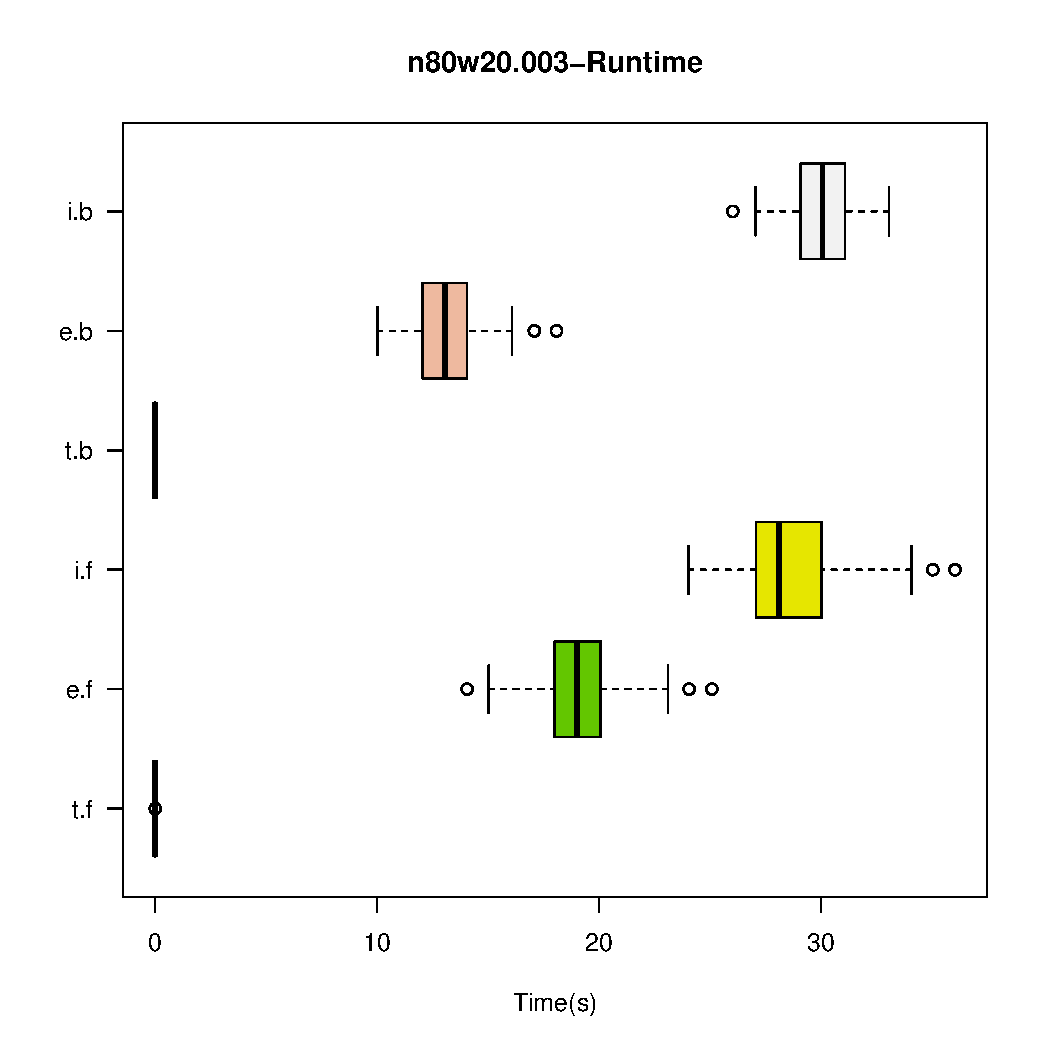
\includegraphics[width=0.6\textwidth,keepaspectratio]{{II/n80w20.003/n80w20.003-CpuTime}.pdf}
% \captionof{figure}{n80w20.003 - Runtime boxplots for the different iterative improvement algorithms}
% \end{center}

% \begin{center}
% 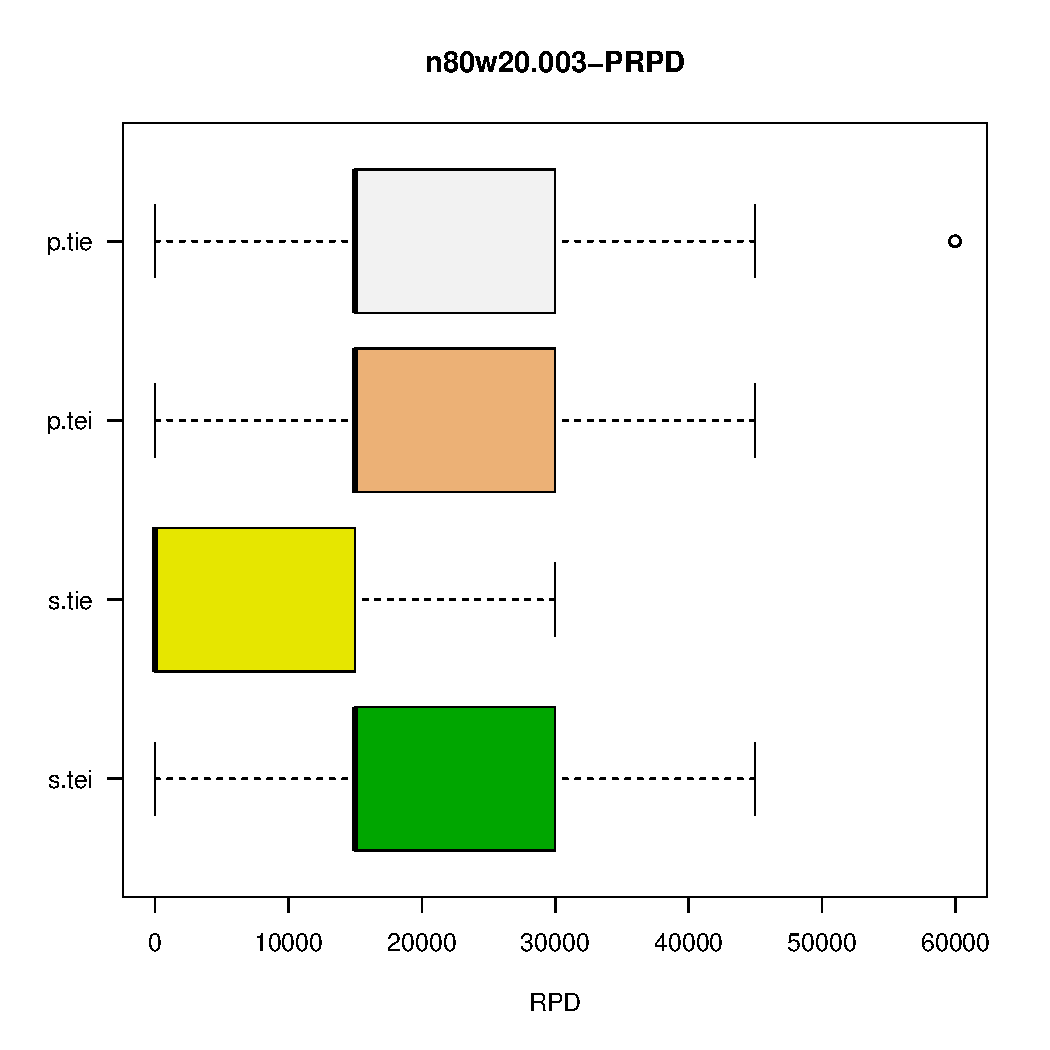
\includegraphics[width=0.6\textwidth,keepaspectratio]{{II/n80w20.003/n80w20.003-PRPD}.pdf}
% \captionof{figure}{n80w20.003 - PRPD boxplots for the different iterative improvement algorithms}
% \end{center}

% \begin{center}
% \begin{tabular}{|l|l|}
% \hline
% \textbf{Test} & \textbf{P-Value} \\
% \hline
% First vs best - Transpose&3.95591160889952e-18\\
% \hline
% First vs best - Exchange&6.21747363653032e-18\\
% \hline
% First vs best - Insert&6.2952945764779e-08\\
% \hline
% Exchange vs Insert - First&3.9556885406462e-18\\
% \hline
% Exchange vs Insert - Best&3.95591160889952e-18\\
% \hline
% \end{tabular}
% \captionof{table}{n80w20.003 - Results of Wilcoxon paired signed rank test}
% \label{tab:w.3}
% \end{center}

% \subsubsection{n80w20.004}
% \begin{center}
% 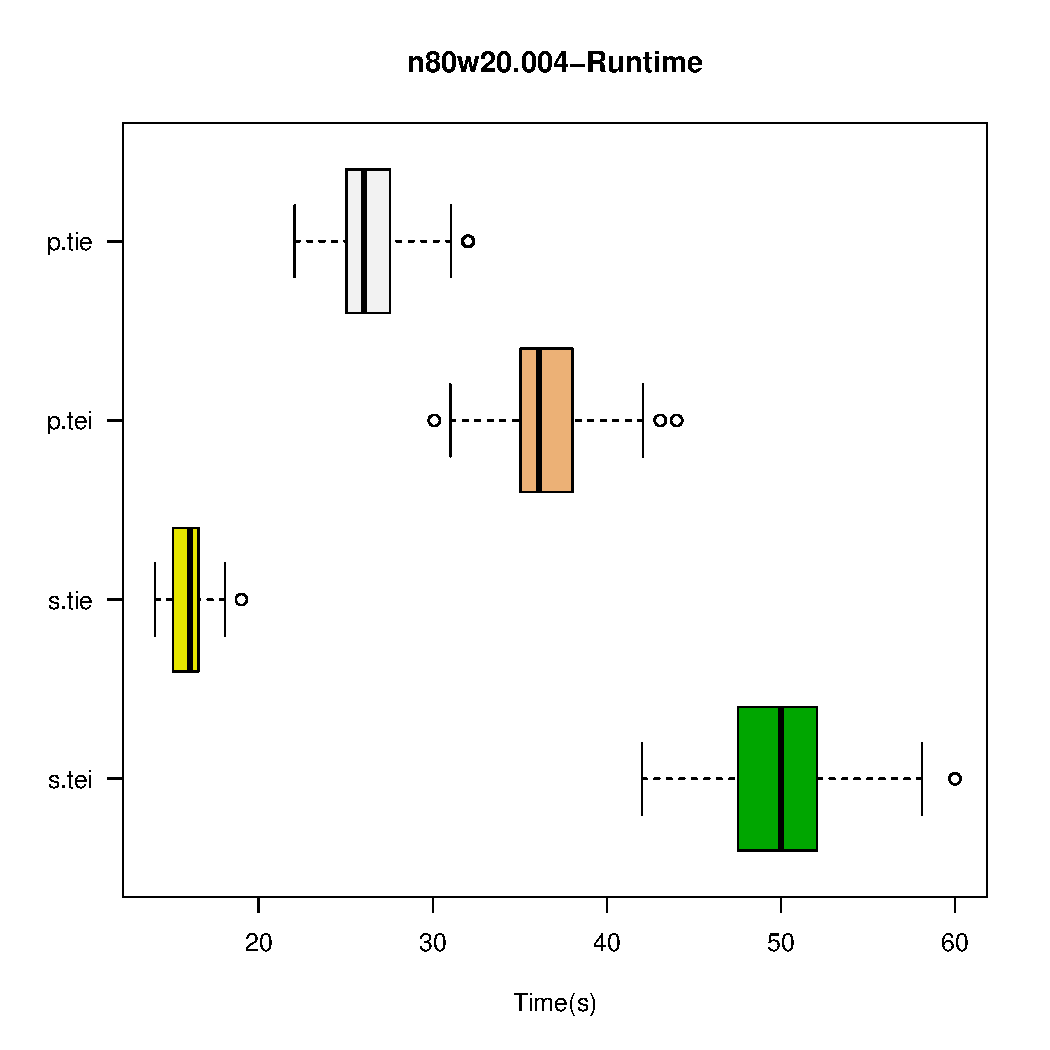
\includegraphics[width=0.6\textwidth,keepaspectratio]{{II/n80w20.004/n80w20.004-CpuTime}.pdf}
% \captionof{figure}{n80w20.004 - Runtime boxplots for the different iterative improvement algorithms}
% \end{center}

% \begin{center}
% 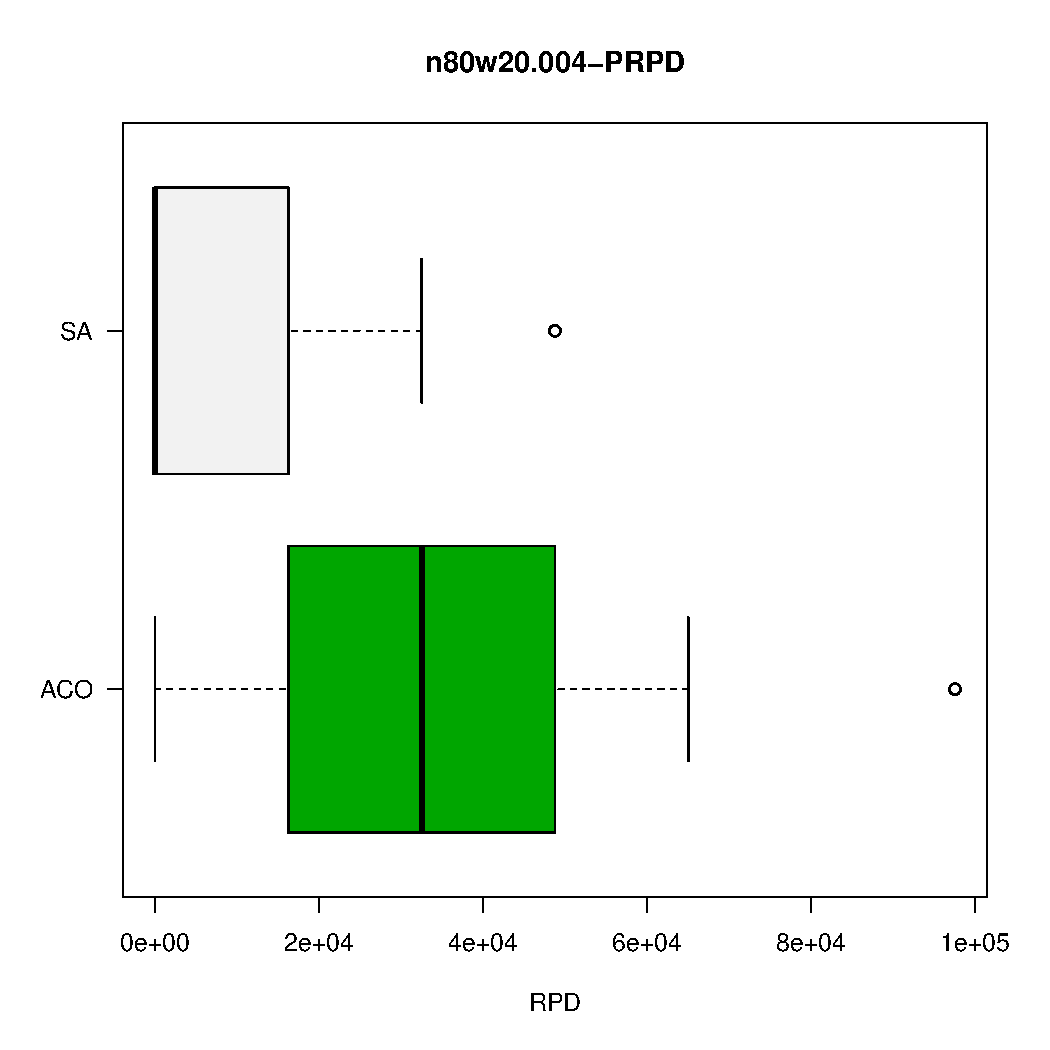
\includegraphics[width=0.6\textwidth,keepaspectratio]{{II/n80w20.004/n80w20.004-PRPD}.pdf}
% \captionof{figure}{n80w20.001 - PRPD boxplots for the different iterative improvement algorithms}
% \end{center}

% \begin{center}
% \begin{tabular}{|l|l|}
% \hline
% \textbf{Test} & \textbf{P-Value} \\
% \hline
% First vs best - Transpose&4.33123080260219e-18\\
% \hline
% First vs best - Exchange&1.5356610755813e-16\\
% \hline
% First vs best - Insert&4.27702026764362e-14\\
% \hline
% Exchange vs Insert - First&5.59593516960623e-18\\
% \hline
% Exchange vs Insert - Best&3.95591160889952e-18\\
% \hline
% \end{tabular}
% \captionof{table}{n80w20.004 - Results of Wilcoxon paired signed rank test}
% \label{tab:w.4}
% \end{center}

% \subsubsection{n80w20.005}
% \begin{center}
% 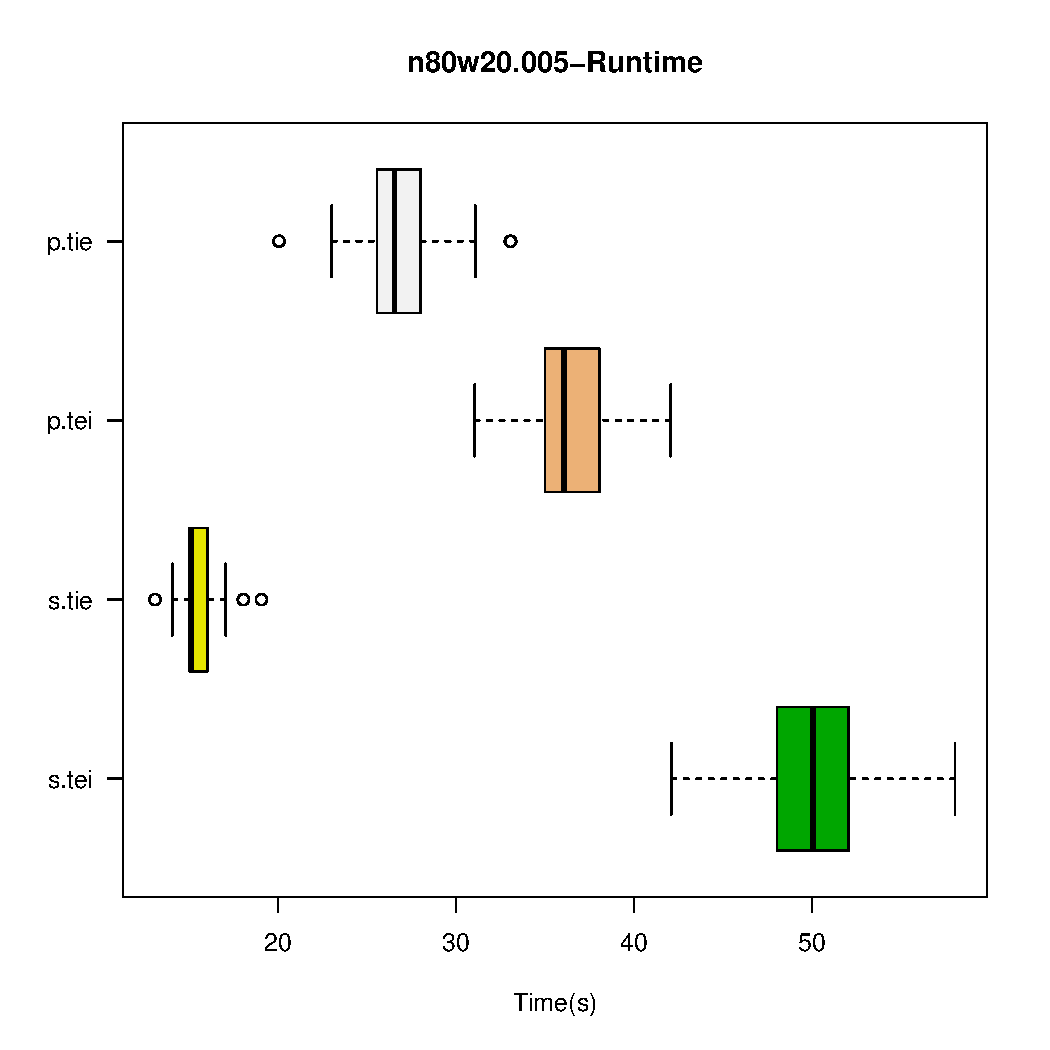
\includegraphics[width=0.6\textwidth,keepaspectratio]{{II/n80w20.005/n80w20.005-CpuTime}.pdf}
% \captionof{figure}{n80w20.005 - Runtime boxplots for the different iterative improvement algorithms}
% \end{center}

% \begin{center}
% 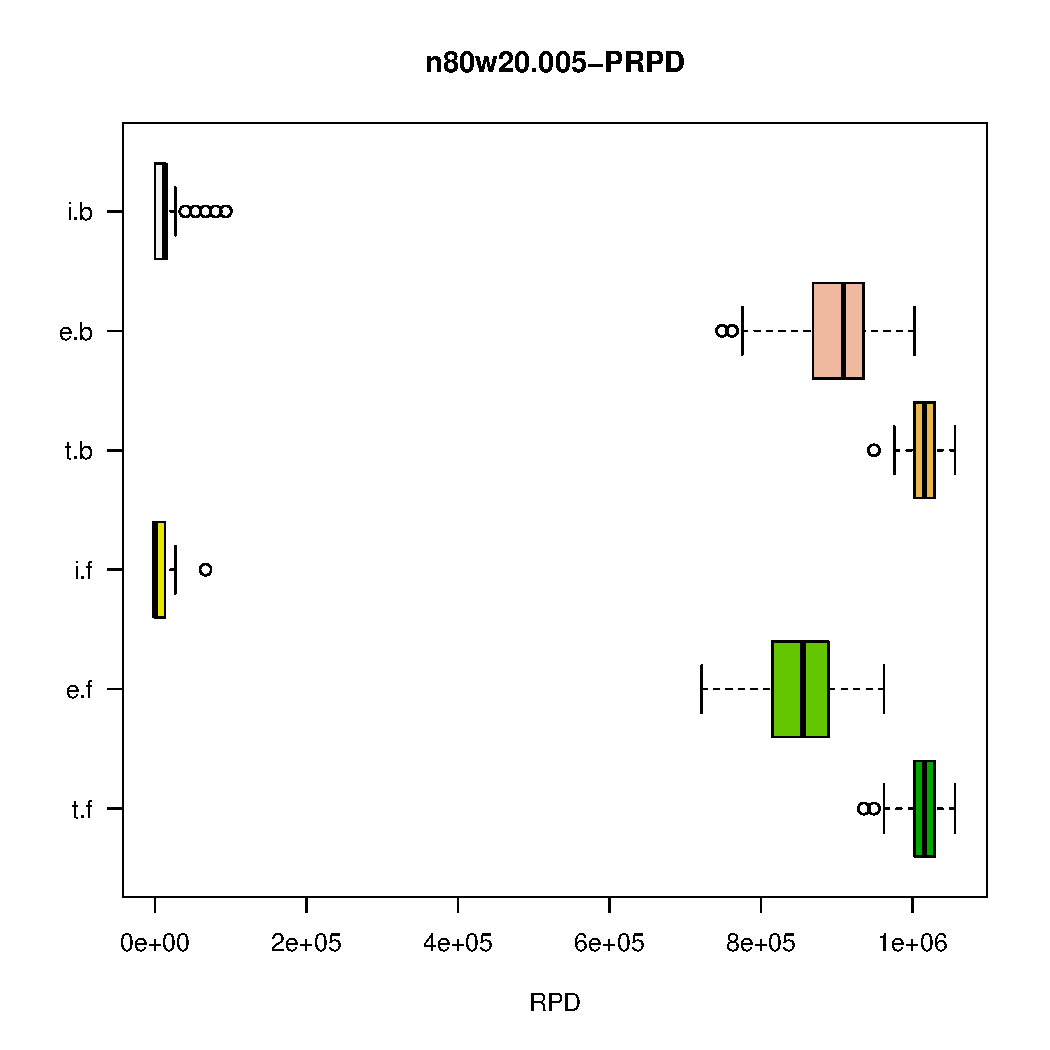
\includegraphics[width=0.6\textwidth,keepaspectratio]{{II/n80w20.005/n80w20.005-PRPD}.pdf}
% \captionof{figure}{n80w20.005 - PRPD boxplots for the different iterative improvement algorithms}
% \end{center}

% \begin{center}
% \begin{tabular}{|l|l|}
% \hline
% \textbf{Test} & \textbf{P-Value} \\
% \hline
% First vs best - Transpose&4.46398542390809e-18\\
% \hline
% First vs best - Exchange&4.74166029806301e-18\\
% \hline
% First vs best - Insert&4.0369131744045e-10\\
% \hline
% Exchange vs Insert - First&4.74166029806301e-18\\
% \hline
% Exchange vs Insert - Best&3.95591160889952e-18\\
% \hline
% \end{tabular}
% \captionof{table}{n80w20.005 - Results of Wilcoxon paired signed rank test}
% \label{tab:w.5}
% \end{center}

% \subsubsection{n80w200.001}
% \begin{center}
% \includegraphics[width=0.6\textwidth,keepaspectratio]{{II/n80w200.001/n80w200.001-CpuTime}.pdf}
% \captionof{figure}{n80w200.001 - Runtime boxplots for the different iterative improvement algorithms}
% \end{center}

% \begin{center}
% \includegraphics[width=0.6\textwidth,keepaspectratio]{{II/n80w200.001/n80w200.001-PRPD}.pdf}
% \captionof{figure}{n80w200.001 - PRPD boxplots for the different iterative improvement algorithms}
% \end{center}

% \begin{center}
% \begin{tabular}{|l|l|}
% \hline
% \textbf{Test} & \textbf{P-Value} \\
% \hline
% First vs best - Transpose&4.07730530936212e-18\\
% \hline
% First vs best - Exchange&2.17457280454137e-17\\
% \hline
% First vs best - Insert&3.95591160889952e-18\\
% \hline
% Exchange vs Insert - First&3.95591160889952e-18\\
% \hline
% Exchange vs Insert - Best&3.95591160889952e-18\\
% \hline
% \end{tabular}
% \captionof{table}{n80w200.001 - Results of Wilcoxon paired signed rank test}
% \label{tab:w.6}
% \end{center}

% \subsubsection{n80w200.002}
% \begin{center}
% \includegraphics[width=0.6\textwidth,keepaspectratio]{{II/n80w200.002/n80w200.002-CpuTime}.pdf}
% \captionof{figure}{n80w200.002 - Runtime boxplots for the different iterative improvement algorithms}
% \end{center}

% \begin{center}
% \includegraphics[width=0.6\textwidth,keepaspectratio]{{II/n80w200.002/n80w200.002-PRPD}.pdf}
% \captionof{figure}{n80w200.002 - PRPD boxplots for the different iterative improvement algorithms}
% \end{center}

% \begin{center}
% \begin{tabular}{|l|l|}
% \hline
% \textbf{Test} & \textbf{P-Value} \\
% \hline
% First vs best - Transpose&5.19043683699158e-18\\
% \hline
% First vs best - Exchange&4.6720416035814e-17\\
% \hline
% First vs best - Insert&3.95591160889952e-18\\
% \hline
% Exchange vs Insert - First&3.95591160889952e-18\\
% \hline
% Exchange vs Insert - Best&3.95591160889952e-18\\
% \hline
% \end{tabular}
% \captionof{table}{n80w200.002 - Results of Wilcoxon paired signed rank test}
% \label{tab:w.7}
% \end{center}

% \subsubsection{n80w200.003}
% \begin{center}
% \includegraphics[width=0.6\textwidth,keepaspectratio]{{II/n80w200.003/n80w200.003-CpuTime}.pdf}
% \captionof{figure}{n80w200.003 - Runtime boxplots for the different iterative improvement algorithms}
% \end{center}

% \begin{center}
% \includegraphics[width=0.6\textwidth,keepaspectratio]{{II/n80w200.003/n80w200.003-PRPD}.pdf}
% \captionof{figure}{n80w200.003 - PRPD boxplots for the different iterative improvement algorithms}
% \end{center}

% \begin{center}
% \begin{tabular}{|l|l|}
% \hline
% \textbf{Test} & \textbf{P-Value} \\
% \hline
% First vs best - Transpose&4.33123080260219e-18\\
% \hline
% First vs best - Exchange&7.01070639830382e-18\\
% \hline
% First vs best - Insert&3.95591160889952e-18\\
% \hline
% Exchange vs Insert - First&3.95591160889952e-18\\
% \hline
% Exchange vs Insert - Best&3.95591160889952e-18\\
% \hline
% \end{tabular}
% \captionof{table}{n80w200.003 - Results of Wilcoxon paired signed rank test}
% \label{tab:w.8}
% \end{center}

% \subsubsection{n80w200.004}
% \begin{center}
% 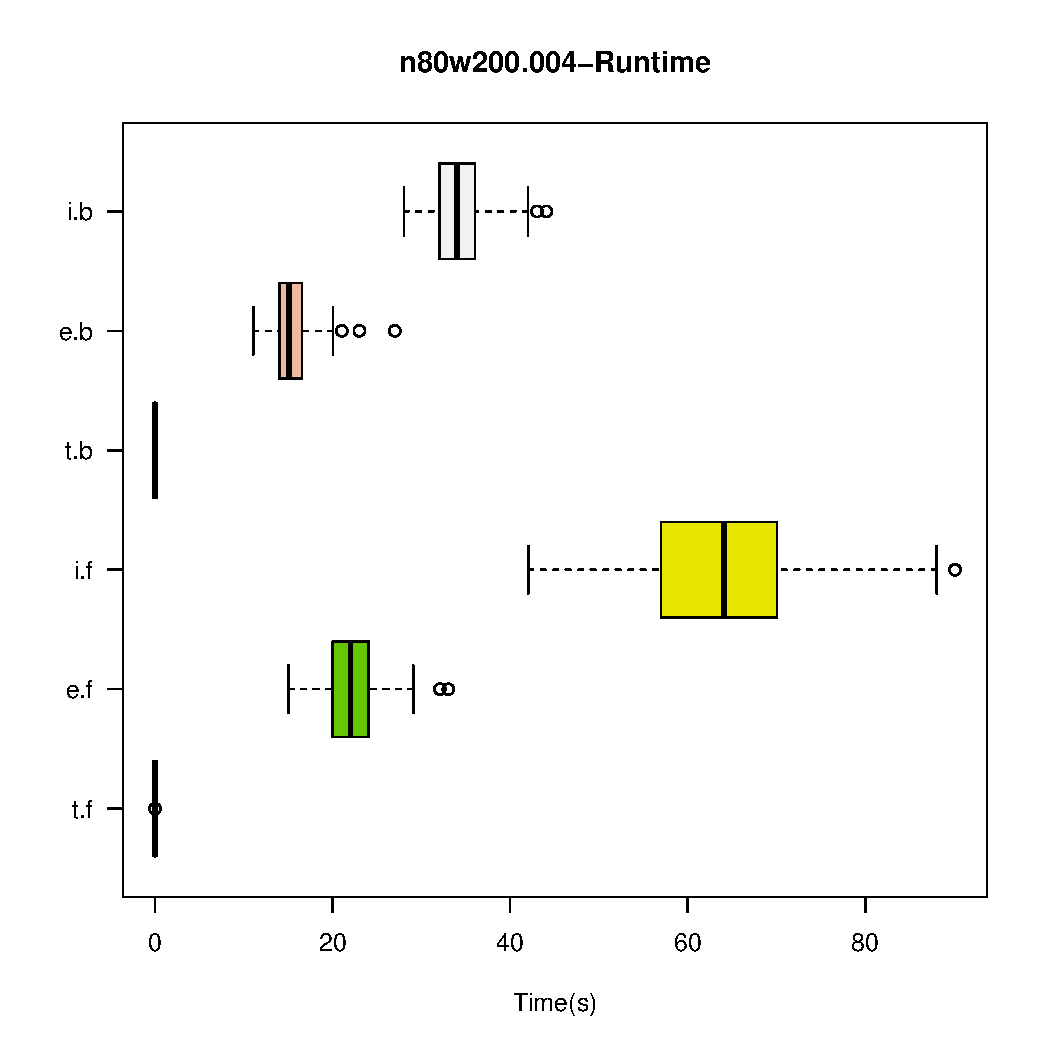
\includegraphics[width=0.6\textwidth,keepaspectratio]{{II/n80w200.004/n80w200.004-CpuTime}.pdf}
% \captionof{figure}{n80w200.004 - Runtime boxplots for the different iterative improvement algorithms}
% \end{center}

% \begin{center}
% 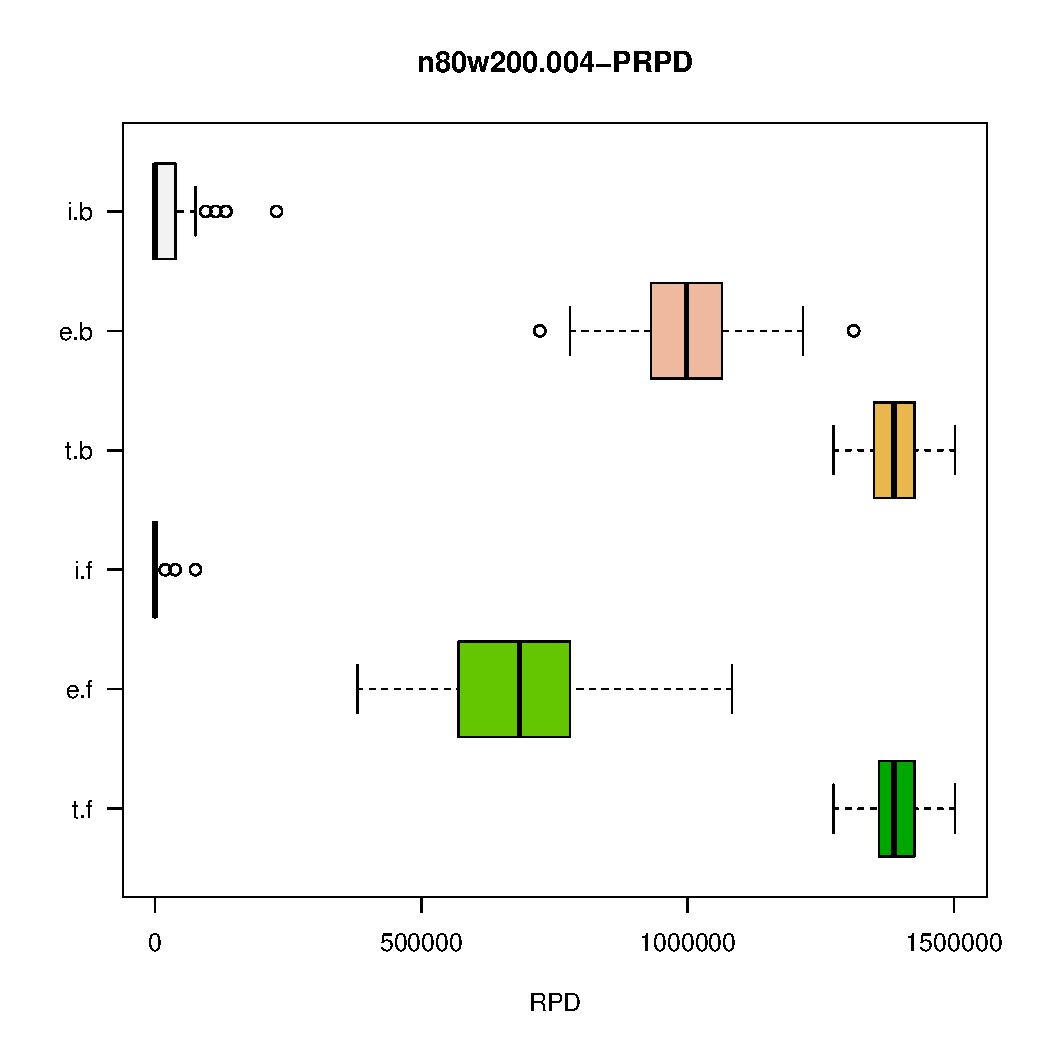
\includegraphics[width=0.6\textwidth,keepaspectratio]{{II/n80w200.004/n80w200.004-PRPD}.pdf}
% \captionof{figure}{n80w200.001 - PRPD boxplots for the different iterative improvement algorithms}
% \end{center}

% \begin{center}
% \begin{tabular}{|l|l|}
% \hline
% \textbf{Test} & \textbf{P-Value} \\
% \hline
% First vs best - Transpose&4.33123080260219e-18\\
% \hline
% First vs best - Exchange&2.4473398426105e-17\\
% \hline
% First vs best - Insert&3.95591160889952e-18\\
% \hline
% Exchange vs Insert - First&3.95591160889952e-18\\
% \hline
% Exchange vs Insert - Best&3.95591160889952e-18\\
% \hline
% \end{tabular}
% \captionof{table}{n80w200.004 - Results of Wilcoxon paired signed rank test}
% \label{tab:w.9}
% \end{center}

% \subsubsection{n80w200.005}
% \begin{center}
% 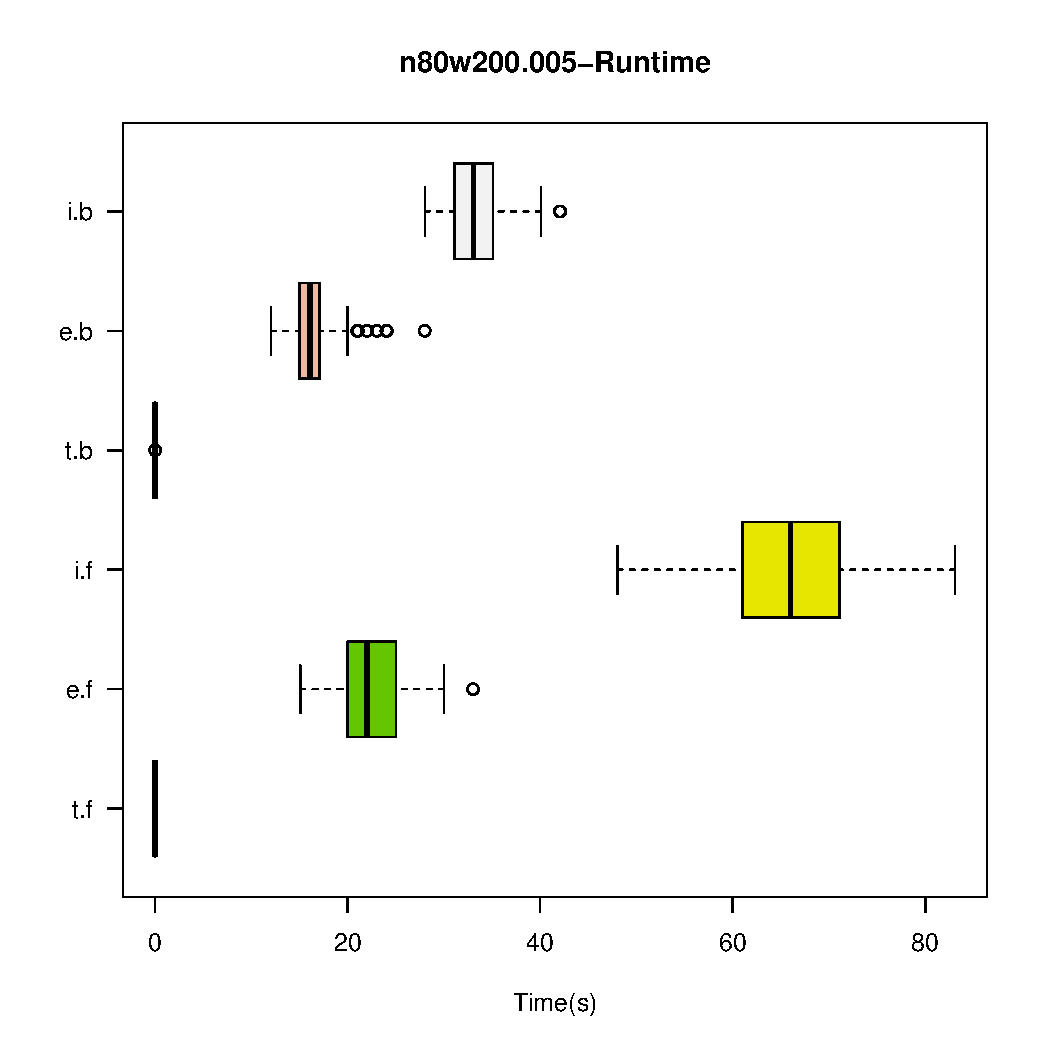
\includegraphics[width=0.6\textwidth,keepaspectratio]{{II/n80w200.005/n80w200.005-CpuTime}.pdf}
% \captionof{figure}{n80w200.005 - Runtime boxplots for the different iterative improvement algorithms}
% \end{center}

% \begin{center}
% 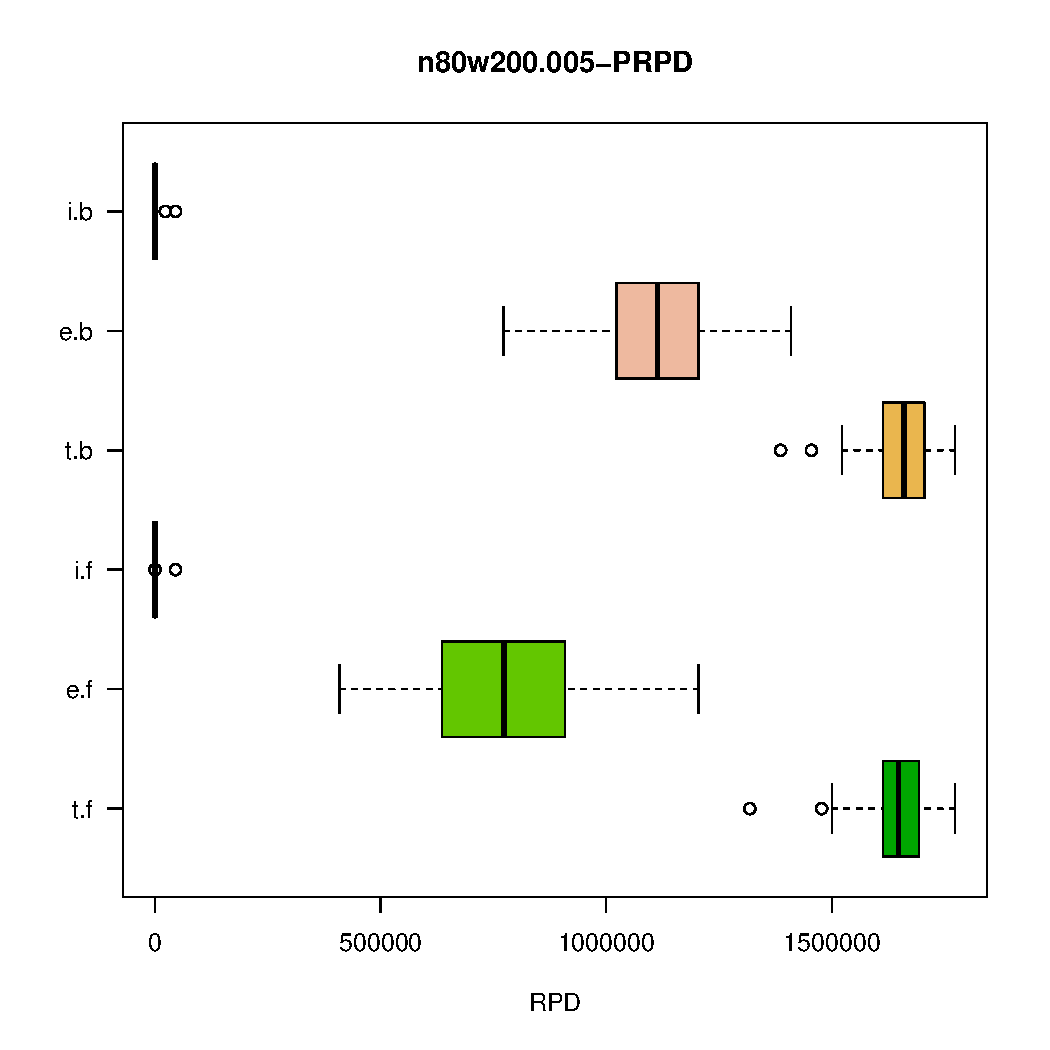
\includegraphics[width=0.6\textwidth,keepaspectratio]{{II/n80w200.005/n80w200.005-PRPD}.pdf}
% \captionof{figure}{n80w200.005 - PRPD boxplots for the different iterative improvement algorithms}
% \end{center}

% \begin{center}
% \begin{tabular}{|l|l|}
% \hline
% \textbf{Test} & \textbf{P-Value} \\
% \hline
% First vs best - Transpose&4.74166029806301e-18\\
% \hline
% First vs best - Exchange&1.40854365025687e-16\\
% \hline
% First vs best - Insert&3.95591160889952e-18\\
% \hline
% Exchange vs Insert - First&3.95591160889952e-18\\
% \hline
% Exchange vs Insert - Best&3.95591160889952e-18\\
% \hline
% \end{tabular}
% \captionof{table}{n80w200.005 - Results of Wilcoxon paired signed rank test}
% \label{tab:w.10}
% \end{center}

% \subsection{Statistics}

% \subsubsection{Transpose-First Improvement}
% \begin{center}
% \begin{tabular}{|l|c|l|l|}
% \hline
% \textbf{Instance}& \textbf{\% Infeasible} & $\mathbf{\bar{PRDP}}$ &$\mathbf{\bar{Runtime}}$\\
% \hline
% n80w20.001&1&1229712.6&0.0100035563\\
% \hline
% n80w20.002&1&1028075.17&0.0095843375\\
% \hline
% n80w20.003&1&1132968.5&0.0098099452\\
% \hline
% n80w20.005&1&1010681.79&0.0097989762\\
% \hline
% n80w20.004&1&1226174.6&0.0094877067\\
% \hline
% n80w200.001&1&1467634.1&0.0098152878\\
% \hline
% n80w200.002&1&1504523.7&0.0099101404\\
% \hline
% n80w200.004&1&1388037.6&0.0098893615\\
% \hline
% n80w200.003&1&1567210.5&0.0097697727\\
% \hline
% n80w200.005&1&1644110.9&0.0097550971\\
% \hline
% \end{tabular}
% \captionof{table}{Statistics summary for iterative improvement algorithm with Transpose neighborhood and First Improvement pivoting rule}
% \label{tab:t.f}
% \end{center}

% \subsubsection{Transpose-Best Improvement}
% \begin{center}
% \begin{tabular}{|l|c|l|l|}
% \hline
% \textbf{Instance}& \textbf{\% Infeasible} & $\mathbf{\bar{PRDP}}$ &$\mathbf{\bar{Runtime}}$\\
% \hline
% n80w20.001&1&1236039.3&0.014545497\\
% \hline
% n80w20.002&1&1033090.48&0.0145450422\\
% \hline
% n80w20.003&1&1137758.7&0.014536776\\
% \hline
% n80w20.005&1&1014818.46&0.014947609\\
% \hline
% n80w20.004&1&1232996&0.015151286\\
% \hline
% n80w200.001&1&1476994.8&0.0147534638\\
% \hline
% n80w200.002&1&1511281&0.014884921\\
% \hline
% n80w200.004&1&1392023.3&0.0146445173\\
% \hline
% n80w200.003&1&1575355.5&0.0143582468\\
% \hline
% n80w200.005&1&1653419.6&0.0150098656\\
% \hline
% \end{tabular}
% \captionof{table}{Statistics summary for iterative improvement algorithm with Transpose neighborhood and Best Improvement pivoting rule}
% \label{tab:t.b}
% \end{center}

% \subsubsection{Exchange-First Improvement}
% \begin{center}
% \begin{tabular}{|l|c|l|l|}
% \hline
% \textbf{Instance}& \textbf{\% Infeasible} & $\mathbf{\bar{PRDP}}$ &$\mathbf{\bar{Runtime}}$\\
% \hline
% n80w20.001&1&1035718.78&18.390814\\
% \hline
% n80w20.002&1&884386.3&18.198632\\
% \hline
% n80w20.003&1&956518.77&18.913801\\
% \hline
% n80w20.005&1&849054.52&19.043496\\
% \hline
% n80w20.004&1&1030411.56&19.660314\\
% \hline
% n80w200.001&1&661322.18&23.117446\\
% \hline
% n80w200.002&1&813339.6&22.552976\\
% \hline
% n80w200.004&1&679489.06&22.068859\\
% \hline
% n80w200.003&1&697450.03&24.338257\\
% \hline
% n80w200.005&1&760027.65&22.348975\\
% \hline
% \end{tabular}
% \captionof{table}{Statistics summary for iterative improvement algorithm with Exchange neighborhood and First Improvement pivoting rule}
% \label{tab:e.f}
% \end{center}

% \subsubsection{Exchange-Best Improvement}
% \begin{center}
% \begin{tabular}{|l|c|l|l|}
% \hline
% \textbf{Instance}& \textbf{\% Infeasible} & $\mathbf{\bar{PRDP}}$ &$\mathbf{\bar{Runtime}}$\\
% \hline
% n80w20.001&1&1086217.68&13.091453\\
% \hline
% n80w20.002&1&901762.05&13.365301\\
% \hline
% n80w20.003&1&1017243.86&13.267128\\
% \hline
% n80w20.005&1&895720.53&13.5824245\\
% \hline
% n80w20.004&1&1084080.4&14.189582\\
% \hline
% n80w200.001&1&1022433.76&16.418229\\
% \hline
% n80w200.002&1&1075649.94&16.028712\\
% \hline
% n80w200.004&1&994703.67&15.518766\\
% \hline
% n80w200.003&1&1094460.9&16.16696\\
% \hline
% n80w200.005&1&1110949.86&16.566802\\
% \hline
% \end{tabular}
% \captionof{table}{Statistics summary for iterative improvement algorithm with Exchange neighborhood and Best Improvement pivoting rule}
% \label{tab:e.b}
% \end{center}

% \subsubsection{Insert-First Improvement}
% \begin{center}
% \begin{tabular}{|l|c|l|l|}
% \hline
% \textbf{Instance}& \textbf{\% Infeasible} & $\mathbf{\bar{PRDP}}$ &$\mathbf{\bar{Runtime}}$\\
% \hline
% n80w20.001&0.65&16070.27322082&25.88279\\
% \hline
% n80w20.002&0.83&11803.71462682&28.509938\\
% \hline
% n80w20.003&0.83&21587.617&28.579453\\
% \hline
% n80w20.005&0.32&4945.642107&28.672083\\
% \hline
% n80w20.004&0.49&10894.01867489&28.474429\\
% \hline
% n80w200.001&0.22&6119.9927045&59.544212\\
% \hline
% n80w200.002&0&11.2561521&64.580306\\
% \hline
% n80w200.004&0.11&3049.80805246&63.942238\\
% \hline
% n80w200.003&0.01&437.87774695&63.687806\\
% \hline
% n80w200.005&0.01&464.62990671&66.084369\\
% \hline
% \end{tabular}
% \captionof{table}{Statistics summary for iterative improvement algorithm with Insert neighborhood and First Improvement pivoting rule}
% \label{tab:i.f}
% \end{center}

% \subsubsection{Insert-Best Improvement}
% \begin{center}
% \begin{tabular}{|l|c|l|l|}
% \hline
% \textbf{Instance}& \textbf{\% Infeasible} & $\mathbf{\bar{PRDP}}$ &$\mathbf{\bar{Runtime}}$\\
% \hline
% n80w20.001&0.56&14772.44442862&28.769951\\
% \hline
% n80w20.002&0.84&16009.51797952&30.159812\\
% \hline
% n80w20.003&0.89&26984.256&30.197019\\
% \hline
% n80w20.005&0.52&10159.3062354&30.776906\\
% \hline
% n80w20.004&0.59&18861.32619536&31.013\\
% \hline
% n80w200.001&0.37&21195.2243605&33.031965\\
% \hline
% n80w200.002&0&13.2172159&33.011011\\
% \hline
% n80w200.004&0.42&23019.4946845&34.123681\\
% \hline
% n80w200.003&0.12&7740.06242146&34.080592\\
% \hline
% n80w200.005&0.07&2516.0079072&33.450537\\
% \hline
% \end{tabular}
% \captionof{table}{Statistics summary for iterative improvement algorithm with Insert neighborhood and Best Improvement pivoting rule}
% \label{tab:i.b}
% \end{center}

% \subsection{Results discussion}
% By looking at tables \ref{tab:t.f}, \ref{tab:t.b}, \ref{tab:e.f}, \ref{tab:e.b} \ref{tab:i.f}, \ref{tab:i.b} on can see that:
% \begin{itemize}
% \item The neighborhood type has a strong influence on the both the time complexity of the algorithm and the generated solution quality. This is due to the size of the different neighborhoods ($n=80$):
%       \begin{itemize}
%         \item Transpose - $(n-1)$
%         \item Exchange - $\frac{n\cdot(n-1)}{2}$
%         \item Insert - $(n-1)^2$
%       \end{itemize}
% The different size of the neighborhoods corresponds to different degrees of exploration (diversification).
      
% \item Transpose and Exchange neighborhoods have smaller runtimes but a percentage of infeasible runs equal to 1. 
% Both the algorithm do not allow to find a feasible solution but the Exchange algorithm constructs solutions with a better quality (reduced, but not yet null, constraint violations and total travel time).

% \item Insert is the only neighborhood type that allows to generate solutions that are both feasible and closer to the global optima.

% \item The first-improvement pivoting rule is generally slower than the best-improvement one, when considering the same neighborhood type.
% This is due to the fact that, with the first-improvement pivoting rule, smaller improvement are made to the solution at each iteration, thus requiring and higher number of iteration to converge to a local optima, with respect to the case where the best improvement is chosen at each time step.

% \item The quality of the solutions generated using the first-improvement pivoting rule is slightly better thant those generated using the best-improvement one.

% \item Tables \ref{tab:w.1}, \ref{tab:w.2}, \ref{tab:w.3}, \ref{tab:w.4}, \ref{tab:w.5}, \ref{tab:w.6}, \ref{tab:w.7}, \ref{tab:w.8}, \ref{tab:w.9}, \ref{tab:w.10} contain, in any case, p-values considerably smaller than the significance level ($\alpha=0.05$). 

% This implies that the null hypothesis corresponding to the equality of the median values of the differences of the two distributions can be rejected, hence assessing the existence of a statistically significant difference among the solution quality generated by analyzed algorithms.

% \item By looking at the Cpu time, one can easily see that the instances \emph{n80w20.X} have lower runtimes than the \emph{n80w200.X} ones. They can then be considered, with respect to the iterative improvement algorithms, simpler instances with respect to the latter.

% \end{itemize}

% An Iterative Improvement algorithm generally starts from a candidate solution, which can be either generated randomly or using an heuristic, and improves the evaluation of the solution at each step by modifying the solution structure , until a local optimum is reached.

% In the previous problem, I considered different kinds of 2-opt neighborhood, and different pivoting rules.

% This means that, at each step, a new solution is constructed from the current best by modifying only two solution components (with Transpose,Exchange or Insert operations) and only the first/best improving solution will become the new best soluion.

% The main limitation of such kind of algorithms is that they tend to get stuck in solutions that are locally optimum but not globally.

% Provided that:
% \begin{itemize}
% \item A global optimum is optimal with respect to any kind of neighborhood. 
% \item A solution that is locally optimal with respect to a neighborhood may not be optimal with respect to other kinds of neighborhood
% \end{itemize}
% by dynamically changing the neighborhood type an algorithm is able to escape local optima.

% This section will analyse the results of the execution of two variable neighborhood descent algorithm, based on the previously analyzed iterative improvement algorithms :
% \begin{itemize}
% \item \textbf{Standard Variable Neighborhood Descent} (i.e. Changing neighborhood when a local optimum is encoutered, until the neighborhood chain is terminated and going back to the smallest neighborhood every time the local optimum is escaped.)
% \item \textbf{Piped Variable Neighborhood Descent} (i.e. Using the locally optimum solution found using one neighborhood type in the chain as the initial solution for the following type.)
% \end{itemize}
% The same metrics as in \ref{subsec:metric} will be used to evaluate the algorithms.

% \subsection{Experiment results}
% \subsubsection{n80w20.001}
% \begin{center}
% \includegraphics[width=0.6\textwidth,keepaspectratio]{{VND/n80w20.001/n80w20.001-CpuTime}.pdf}
% \captionof{figure}{n80w20.001 - Runtime boxplots for the different variable neighborhood descent algorithms}
% \end{center}

% \begin{center}
% \includegraphics[width=0.6\textwidth,keepaspectratio]{{VND/n80w20.001/n80w20.001-PRPD}.pdf}
% \captionof{figure}{n80w20.001 - PRPD boxplots for the different variable neighborhood descent algorithms}
% \end{center}

% \begin{center}
% \begin{tabular}{|l|l|}
% \hline
% \textbf{Test} & \textbf{P-Value} \\
% \hline
% Tei vs Tie - Standard&3.95591160889952e-18\\
% \hline
% Tei vs Tie - Piped&3.9556885406462e-18\\
% \hline
% Standard vs Piped - Tei&3.95591160889952e-18\\
% \hline
% Standard vs Piped - Tie&3.95591160889952e-18\\
% \hline
% \end{tabular}
% \captionof{table}{n80w20.001 - Results of Wilcoxon paired signed rank test}
% \label{tab:w.11}
% \end{center}

% \subsubsection{n80w20.002}
% \begin{center}
% \includegraphics[width=0.6\textwidth,keepaspectratio]{{VND/n80w20.002/n80w20.002-CpuTime}.pdf}
% \captionof{figure}{n80w20.002 - Runtime boxplots for the different variable neighborhood descent algorithms}
% \end{center}

% \begin{center}
% \includegraphics[width=0.6\textwidth,keepaspectratio]{{VND/n80w20.002/n80w20.002-PRPD}.pdf}
% \captionof{figure}{n80w20.002 - PRPD boxplots for the different variable neighborhood descent algorithms}
% \end{center}

% \begin{center}
% \begin{tabular}{|l|l|}
% \hline
% \textbf{Test} & \textbf{P-Value} \\
% \hline
% Tei vs Tie - Standard&3.9556885406462e-18\\
% \hline
% Tei vs Tie - Piped&3.95591160889952e-18\\
% \hline
% Standard vs Piped - Tei&3.95591160889952e-18\\
% \hline
% Standard vs Piped - Tie&3.95591160889952e-18\\
% \hline
% \end{tabular}
% \captionof{table}{n80w20.002 - Results of Wilcoxon paired signed rank test}
% \label{tab:w.12}
% \end{center}

% \subsubsection{n80w20.003}
% \begin{center}
% \includegraphics[width=0.6\textwidth,keepaspectratio]{{VND/n80w20.003/n80w20.003-CpuTime}.pdf}
% \captionof{figure}{n80w20.003 - Runtime boxplots for the different variable neighborhood descent algorithms}
% \end{center}

% \begin{center}
% \includegraphics[width=0.6\textwidth,keepaspectratio]{{VND/n80w20.003/n80w20.003-PRPD}.pdf}
% \captionof{figure}{n80w20.003 - PRPD boxplots for the different variable neighborhood descent algorithms}
% \end{center}

% \begin{center}
% \begin{tabular}{|l|l|}
% \hline
% \textbf{Test} & \textbf{P-Value} \\
% \hline
% Tei vs Tie - Standard&3.9552424399092e-18\\
% \hline
% Tei vs Tie - Piped&3.95591160889952e-18\\
% \hline
% Standard vs Piped - Tei&3.95591160889952e-18\\
% \hline
% Standard vs Piped - Tie&3.95591160889952e-18\\
% \hline
% \end{tabular}
% \captionof{table}{n80w20.003 - Results of Wilcoxon paired signed rank test}
% \label{tab:w.13}
% \end{center}

% \subsubsection{n80w20.004}
% \begin{center}
% \includegraphics[width=0.6\textwidth,keepaspectratio]{{VND/n80w20.004/n80w20.004-CpuTime}.pdf}
% \captionof{figure}{n80w20.004 - Runtime boxplots for the different variable neighborhood descent algorithms}
% \end{center}

% \begin{center}
% \includegraphics[width=0.6\textwidth,keepaspectratio]{{VND/n80w20.004/n80w20.004-PRPD}.pdf}
% \captionof{figure}{n80w20.004 - PRPD boxplots for the different variable neighborhood descent algorithms}
% \end{center}

% \begin{center}
% \begin{tabular}{|l|l|}
% \hline
% \textbf{Test} & \textbf{P-Value} \\
% \hline
% Tei vs Tie - Standard&3.95591160889952e-18\\
% \hline
% Tei vs Tie - Piped&3.95591160889952e-18\\
% \hline
% Standard vs Piped - Tei&3.95591160889952e-18\\
% \hline
% Standard vs Piped - Tie&3.95591160889952e-18\\
% \hline
% \end{tabular}
% \captionof{table}{n80w20.004 - Results of Wilcoxon paired signed rank test}
% \label{tab:w.14}
% \end{center}

% \subsubsection{n80w20.005}
% \begin{center}
% \includegraphics[width=0.6\textwidth,keepaspectratio]{{VND/n80w20.005/n80w20.005-CpuTime}.pdf}
% \captionof{figure}{n80w20.005 - Runtime boxplots for the different variable neighborhood descent algorithms}
% \end{center}

% \begin{center}
% \includegraphics[width=0.6\textwidth,keepaspectratio]{{VND/n80w20.005/n80w20.005-PRPD}.pdf}
% \captionof{figure}{n80w20.001 - PRPD boxplots for the different variable neighborhood descent algorithms}
% \end{center}

% \begin{center}
% \begin{tabular}{|l|l|}
% \hline
% \textbf{Test} & \textbf{P-Value} \\
% \hline
% Tei vs Tie - Standard&3.95591160889952e-18\\
% \hline
% Tei vs Tie - Piped&3.95591160889952e-18\\
% \hline
% Standard vs Piped - Tei&3.95591160889952e-18\\
% \hline
% Standard vs Piped - Tie&3.95591160889952e-18\\
% \hline
% \end{tabular}
% \captionof{table}{n80w20.005 - Results of Wilcoxon paired signed rank test}
% \label{tab:w.15}
% \end{center}

% \subsubsection{n80w200.001}
% \begin{center}
% \includegraphics[width=0.6\textwidth,keepaspectratio]{{VND/n80w200.001/n80w200.001-CpuTime}.pdf}
% \captionof{figure}{n80w200.001 - Runtime boxplots for the different variable neighborhood descent algorithms}
% \end{center}

% \begin{center}
% \includegraphics[width=0.6\textwidth,keepaspectratio]{{VND/n80w200.001/n80w200.001-PRPD}.pdf}
% \captionof{figure}{n80w200.001 - PRPD boxplots for the different variable neighborhood descent algorithms}
% \end{center}

% \begin{center}
% \begin{tabular}{|l|l|}
% \hline
% \textbf{Test} & \textbf{P-Value} \\
% \hline
% Tei vs Tie - Standard&4.07730530936212e-18\\
% \hline
% Tei vs Tie - Piped&2.92094064174088e-17\\
% \hline
% Standard vs Piped - Tei&2.72456795287507e-16\\
% \hline
% Standard vs Piped - Tie&3.95591160889952e-18\\
% \hline
% \end{tabular}
% \captionof{table}{n80w200.001 - Results of Wilcoxon paired signed rank test}
% \label{tab:w.16}
% \end{center}

% \subsubsection{n80w200.002}
% \begin{center}
% \includegraphics[width=0.6\textwidth,keepaspectratio]{{VND/n80w200.002/n80w200.002-CpuTime}.pdf}
% \captionof{figure}{n80w200.002 - Runtime boxplots for the different variable neighborhood descent algorithms}
% \end{center}

% \begin{center}
% \includegraphics[width=0.6\textwidth,keepaspectratio]{{VND/n80w200.002/n80w200.002-PRPD}.pdf}
% \captionof{figure}{n80w200.002 - PRPD boxplots for the different variable neighborhood descent algorithms}
% \end{center}

% \begin{center}
% \begin{tabular}{|l|l|}
% \hline
% \textbf{Test} & \textbf{P-Value} \\
% \hline
% Tei vs Tie - Standard&3.95591160889952e-18\\
% \hline
% Tei vs Tie - Piped&1.52379449675399e-17\\
% \hline
% Standard vs Piped - Tei&1.74838327736385e-15\\
% \hline
% Standard vs Piped - Tie&3.95591160889952e-18\\
% \hline
% \end{tabular}
% \captionof{table}{n80w200.002 - Results of Wilcoxon paired signed rank test}
% \label{tab:w.17}
% \end{center}

% \subsubsection{n80w200.003}
% \begin{center}
% \includegraphics[width=0.6\textwidth,keepaspectratio]{{VND/n80w200.003/n80w200.003-CpuTime}.pdf}
% \captionof{figure}{n80w200.003 - Runtime boxplots for the different variable neighborhood descent algorithms}
% \end{center}

% \begin{center}
% \includegraphics[width=0.6\textwidth,keepaspectratio]{{VND/n80w200.003/n80w200.003-PRPD}.pdf}
% \captionof{figure}{n80w200.003 - PRPD boxplots for the different variable neighborhood descent algorithms}
% \end{center}

% \begin{center}
% \begin{tabular}{|l|l|}
% \hline
% \textbf{Test} & \textbf{P-Value} \\
% \hline
% Tei vs Tie - Standard&2.04955667109233e-17\\
% \hline
% Tei vs Tie - Piped&2.59611565456869e-17\\
% \hline
% Standard vs Piped - Tei&1.50422804122146e-07\\
% \hline
% Standard vs Piped - Tie&3.95591160889952e-18\\
% \hline
% \end{tabular}
% \captionof{table}{n80w200.003 - Results of Wilcoxon paired signed rank test}
% \label{tab:w.18}
% \end{center}

% \subsubsection{n80w200.004}
% \begin{center}
% \includegraphics[width=0.6\textwidth,keepaspectratio]{{VND/n80w200.004/n80w200.004-CpuTime}.pdf}
% \captionof{figure}{n80w200.004 - Runtime boxplots for the different variable neighborhood descent algorithms}
% \end{center}

% \begin{center}
% \includegraphics[width=0.6\textwidth,keepaspectratio]{{VND/n80w200.004/n80w200.004-PRPD}.pdf}
% \captionof{figure}{n80w200.004 - PRPD boxplots for the different variable neighborhood descent algorithms}
% \end{center}

% \begin{center}
% \begin{tabular}{|l|l|}
% \hline
% \textbf{Test} & \textbf{P-Value} \\
% \hline
% Tei vs Tie - Standard&4.07730530936212e-18\\
% \hline
% Tei vs Tie - Piped&4.29577057320019e-16\\
% \hline
% Standard vs Piped - Tei&5.3075517052254e-11\\
% \hline
% Standard vs Piped - Tie&3.95591160889952e-18\\
% \hline
% \end{tabular}
% \captionof{table}{n80w200.004 - Results of Wilcoxon paired signed rank test}
% \label{tab:w.19}
% \end{center}

% \subsubsection{n80w200.005}
% \begin{center}
% \includegraphics[width=0.6\textwidth,keepaspectratio]{{VND/n80w200.005/n80w200.005-CpuTime}.pdf}
% \captionof{figure}{n80w200.005 - Runtime boxplots for the different variable neighborhood descent algorithms}
% \end{center}

% \begin{center}
% \includegraphics[width=0.6\textwidth,keepaspectratio]{{VND/n80w200.005/n80w200.005-PRPD}.pdf}
% \captionof{figure}{n80w200.001 - PRPD boxplots for the different variable neighborhood descent algorithms}
% \end{center}

% \begin{center}
% \begin{tabular}{|l|l|}
% \hline
% \textbf{Test} & \textbf{P-Value} \\
% \hline
% Tei vs Tie - Standard&1.39380002081336e-17\\
% \hline
% Tei vs Tie - Piped&4.07730530936212e-18\\
% \hline
% Standard vs Piped - Tei&3.72316935219101e-06\\
% \hline
% Standard vs Piped - Tie&3.95591160889952e-18\\
% \hline
% \end{tabular}
% \captionof{table}{n80w200.001 - Results of Wilcoxon paired signed rank test}
% \label{tab:w.20}
% \end{center}

% \subsection{Statistics}
% \subsubsection{Standard-Transpose-Exchange-Insert}
% \begin{center}
% \begin{tabular}{|l|c|l|l|}
% \hline
% \textbf{Instance}& \textbf{\% Infeasible} & $\mathbf{\bar{PRDP}}$ &$\mathbf{\bar{Runtime}}$\\
% \hline
% n80w20.001&0.71&14772.04644164&50.611339\\
% \hline
% n80w20.002&0.88&12888.542&50.727053\\
% \hline
% n80w20.003&0.92&19936.872&50.820348\\
% \hline
% n80w20.004&0.62&17234.94260984&50.049484\\
% \hline
% n80w20.005&0.94&12564.0560428&50.269182\\
% \hline
% n80w200.001&0.28&11212.97389136&49.151249\\
% \hline
% n80w200.002&0.03&629.5853274&51.433949\\
% \hline
% n80w200.003&0.07&1511.56628539&49.082085\\
% \hline
% n80w200.004&0.16&4193.4817209&49.662512\\
% \hline
% n80w200.005&0.01&466.6729061&46.701953\\
% \hline
% \end{tabular}
% \captionof{table}{Statistics summary for variable neighborhood descent algorithm with Transpose-Exchange-Insert neighborhood chain and Standard VND type}
% \label{tab:s.tei}
% \end{center}

% \subsubsection{Standard-Transpose-Insert-Exchange}
% \begin{center}
% \begin{tabular}{|l|c|l|l|}
% \hline
% \textbf{Instance}& \textbf{\% Infeasible} & $\mathbf{\bar{PRDP}}$ &$\mathbf{\bar{Runtime}}$\\
% \hline
% n80w20.001&0.54&10874.77632472&15.268454\\
% \hline
% n80w20.002&0.62&8411.724&15.386641\\
% \hline
% n80w20.003&0.44&7645.295&15.638153\\
% \hline
% n80w20.004&0.39&7153.68881324&15.980347\\
% \hline
% n80w20.005&0.25&3475.2731712&15.55767\\
% \hline
% n80w200.001&0.16&4898.3227617&33.424555\\
% \hline
% n80w200.002&0&11.0430351&32.198479\\
% \hline
% n80w200.003&0.05&1082.1460308&34.345522\\
% \hline
% n80w200.004&0.28&7804.19186258&32.583152\\
% \hline
% n80w200.005&0&10.20227353&34.501294\\
% \hline
% \end{tabular}
% \captionof{table}{Statistics summary for variable neighborhood descent algorithm with Transpose-Insert-Exchange neighborhood chain and Standard VND type}
% \label{tab:s.tie}
% \end{center}

% \subsubsection{Piped-Transpose-Exchange-Insert}
% \begin{center}
% \begin{tabular}{|l|c|l|l|}
% \hline
% \textbf{Instance}& \textbf{\% Infeasible} & $\mathbf{\bar{PRDP}}$ &$\mathbf{\bar{Runtime}}$\\
% \hline
% n80w20.001&0.59&12336.84228578&35.694416\\
% \hline
% n80w20.002&0.94&15603.0142035&36.212393\\
% \hline
% n80w20.003&0.83&19338.924&34.821217\\
% \hline
% n80w20.004&0.55&13170.33921962&36.438959\\
% \hline
% n80w20.005&0.45&6683.336214&36.202891\\
% \hline
% n80w200.001&0.19&5104.3621015&40.772642\\
% \hline
% n80w200.002&0.01&218.8179842&44.241593\\
% \hline
% n80w200.003&0.06&2584.90674231&44.725066\\
% \hline
% n80w200.004&0.17&3430.64506042&43.760992\\
% \hline
% n80w200.005&0.02&693.0136326&42.646023\\
% \hline
% \end{tabular}
% \captionof{table}{Statistics summary for variable neighborhood descent algorithm with Transpose-Exchange-Insert neighborhood chain and Piped VND type}
% \label{tab:p.tei}
% \end{center}

% \subsubsection{Piped-Transpose-Insert-Exchange}
% \begin{center}
% \begin{tabular}{|l|c|l|l|}
% \hline
% \textbf{Instance}& \textbf{\% Infeasible} & $\mathbf{\bar{PRDP}}$ &$\mathbf{\bar{Runtime}}$\\
% \hline
% n80w20.001&0.68&16393.81210394&24.788225\\
% \hline
% n80w20.002&0.81&11667.654&25.902581\\
% \hline
% n80w20.003&0.84&20537.669&26.442309\\
% \hline
% n80w20.004&0.46&8779.79314651&26.424231\\
% \hline
% n80w20.005&0.24&3876.3661498&26.511156\\
% \hline
% n80w200.001&0.21&5917.0312803&52.302366\\
% \hline
% n80w200.002&0.01&626.0983757&56.238843\\
% \hline
% n80w200.003&0.04&867.92563269&58.498874\\
% \hline
% n80w200.004&0.28&6281.58944822&55.867038\\
% \hline
% n80w200.005&0.01&236.8657243&58.331595\\
% \hline
% \end{tabular}
% \captionof{table}{Statistics summary for variable neighborhood descent algorithm with Transpose-Insert-Exchange neighborhood chain and Piped VND type}
% \label{tab:p.tie}
% \end{center}

% \subsection{Results discussion}
% By looking at tables \ref{tab:s.tei}, \ref{tab:s.tie}, \ref{tab:p.tei}, \ref{tab:p.tie} one can see that:
% \begin{itemize}

% \item For some instances (e.g. $n80w20.002$,$n80w20.003$) the algorithm are not able to converge to a feasible solution, as shown in the corresponding boxplots, since the PRPD distribution is centered around 12000-15000, thus indicating the presence of at least 1 constraint violations in most of the cases.

% \item For some other instances (e.g. $n80w20.004$,$n80w20.005$) the algorithms are able to converge to feasible solutions and to the best-known one, but having a right-skewed distribution towards higher values of PRPD.

% \item For the remaining instances, except for some outlier values, the algorithms are able to converge to the best-known solution in most of the runs , even though the average PRPD is not closer to 0. This is due to the fact that the mean of a distribution is sensible to outliers and the penalisation for a constraint violations is extremely high when compared to the mean value.
      
% \item The algorithm ordering in terms of runtimes is $s.tie < p.tie < p.tei < s.tei$ for the  $n80w20.X$ instances while $s.tie < p.tei < s.tei < p.tie$ for $n80w200.X$ ones. The choice to explore the Insert Neighborhood before the Exchange one allows to reduce the computation time for the $n80w20.X$ instances, with a similar solution quality.

% \item The algorithms are more effective on the $n80w200.X$ instances then the $n80w20.X$ once, since they have a lower percentage of infeasible runs and a lower PRPD.

% \item The standard variable neighborhood descent with Transpose-Insert-Exchange neighborhood chain (s.tie) outperforms all the other algorithms in terms of solution quality and runtime.

% \item Tables \ref{tab:w.11}, \ref{tab:w.12}, \ref{tab:w.13}, \ref{tab:w.14}, \ref{tab:w.15}, \ref{tab:w.16}, \ref{tab:w.17}, \ref{tab:w.18}, \ref{tab:w.19}, \ref{tab:w.20} contain, in any case, p-values considerably smaller than the significance level ($\alpha=0.05$). 

% This implies that the null hypothesis corresponding to the equality of the median values of the differences of the two distributions can be rejected, hence assessing the existence of a statistically significant difference among the solution quality generated by analyzed algorithms.

% \item By looking at the Cpu time, one can see that the instances \emph{n80w20.X} have generally lower runtimes than the \emph{n80w200.X} ones. They can then be considered, with respect to the variable neighborhood descent algorithms, simpler (quickier to solve) instances with respect to the latter.

% \end{itemize}



\section{Conclusions}
By combining the results from the previous analysis:
\begin{itemize}
  \item The Iterative Improvement algorithms based on Transpose and Exchange neighborhoods do not allow to find feasible solutions hence they should not be considered for a practical application.
  \item On the other hand, the solution quality generated by the Iterative Improvement algorithm with the Insert neighborhood is similar to those generated by the VND algorithms, regardless of the instances.
  \item On this set of instances, the VND algorithms have a lower runtime than the Iterative Improvement one using Insert neighborhood, hence being similar the resulting solution quality, they should be preferred to the Iterative Improvement ones.
  \item The algorithm that showed the best performances in terms of solution quality and runtime is the Standard Variable Neighborhood Descent with Transpose-Insert-Exchange neighborhood chain.
  \item The usage of average statistics as metrics to measure the quality of the algorithms is strongly biased by the presence of outliers (penalisation, in this case).
\end{itemize}



\bibliographystyle{plain}
\bibliography{References}

\end{document}
